\documentclass[11pt,twoside]{docs/thesis}
%\documentclass[tikz]{standalone}
\usepackage[utf8]{inputenc}
\usepackage[spanish]{babel}
\renewcommand\spanishtablename{Tabla}
\usepackage{enumerate}
\usepackage{longtable}
\usepackage{url}
% \usepackage{hyperref}  aqui estaba hyperref en orden
\usepackage{makeidx}
\usepackage{multicol}
\usepackage{graphics}
%\usepackage{translator}

\usepackage{datetime}
\yyyymmdddate
\usepackage{pdflscape} % provides the landscape environment
\usepackage{ragged2e} % provides \RaggedLeft
\usepackage{hyperref}
\usepackage[intoc, spanish]{nomencl}

% %%%%%%%%%%%%%%%%%%%%%%%%%%%%%%%%%%
% %  Paragraph as another subsubsubsection 2023
% \usepackage{titlesec}
% \titleformat{\paragraph}
% {\normalfont\normalsize\bfseries}{\theparagraph}{1em}{}
% \setcounter{secnumdepth}{4}
% \setcounter{tocdepth}{4}
% \titlespacing*{\paragraph}
% {0pt}{3.25ex plus 1ex minus .2ex}{1.5ex plus .2ex}
% %%%%%%%%%%%%%%%%%%%%%%%%%%%%%%%%%%%




%%%%%%%%%%%%%%%%
% TITULO DEL TRABAJO DE GRADO
%%%%%%%%%%%%%%%%

\titulo{Modelamiento dinámico de la producción ganadera en el Servicio Nacional de Aprendizaje SENA - Seccional Popayán, Cauca}

%\autorA{COD}{Primer Autor}
\autorA{2117293}{Ing. Luis Felipe Guevara Gómez}
%\autorB{COD}{Segundo Autor} %Opcional

%%%%%%%
% FECHA DE ENTREGA
%%%%%%%

\fecha{\today}

%%%%%%%%%%%%%%%%%
% DIRECTOR DEL PROYECTO
% DIRECTOR DE CARRERA
% DECANO
%%%%%%%%%%%%%%%%%

%\directorproyecto{Dr.}{Nombre del Director}
\directorproyecto{Dr.}{Luis Eduardo Tobón Llano}
%\codirectorproyecto{Dr.}{Luis Fernando Macea Mercado}
\directorcarrera{Dr.}{Juan Carlos Martinez Arias}

% TeK
\decanoFIC{Dr.}{Hern\'an Camilo Rocha Ni\~no}

%%%%%%%
% JURADOS
%%%%%%%
\juradoA{Degree.}{pepito perez \#1} % Jurado 1
\juradoB{Degree.}{Pepito perez \#2} % Jurado 2

\usepackage{amsmath,amssymb}             % AMS Math
% \usepackage[french]{babel}
\usepackage[latin1]{inputenc}
\usepackage[T1]{fontenc}
\usepackage{rotating,amsmath,booktabs,graphicx} % March 2023
\usepackage{xcolor}
\usepackage{caption}
\usepackage{subcaption}
% \usepackage{nomenc1}
\usepackage{paralist}
\usepackage{ulem}
\usepackage{etoolbox}
\usepackage[left=1.0in,right=1.0in,top=1.0in,bottom=1.0in,includefoot,includehead,headheight=13.6pt]{geometry}
\renewcommand{\baselinestretch}{1.05}
%  19/10/19
% \newcommand{\squeezeup}{\vspace{-2.5mm}}
% 19/10/19

% Table of contents for each chapter

\usepackage[nottoc, notlof, notlot]{tocbibind}
\usepackage{minitoc}



%%%%%%%%%%%%%%%%%%%%%%%%%%%%%%%%%%%%%%%%%%%%%%%%%%%%%%%%%%%%%%%%%%%
%%%%%%%%%%%%%%%%%%%%%%%%%%%%%%%%%%%%%%%%%%%%%%%%%%%%%%%%%%%%%%%%%%%

\usepackage{pgfgantt}

\definecolor{darkgreen}{RGB}{0,176,80}
\definecolor{lightgreen}{RGB}{169,208,142}
\definecolor{beige}{RGB}{242,242,242}
\definecolor{blue2}{RGB}{189,215,238}
\definecolor{barblue}{RGB}{153,220,254}
\definecolor{groupblue}{RGB}{51,102,254}
\definecolor{linkred}{RGB}{165,0,33}
\definecolor{groupgreen}{RGB}{0,240,0}
\definecolor{bargreen}{RGB}{0,220,0}
\definecolor{tabla1}{RGB}{255,217,102}
\definecolor{tabla2}{RGB}{189,215,238}

\renewcommand\sfdefault{phv}
\renewcommand\mddefault{mc}
%\renewcommand\bfdefault{bc}
\setganttlinklabel{s-s}{S -> S}
\setganttlinklabel{f-s}{F -> S}
\setganttlinklabel{f-f}{F -> F}
\sffamily

%%
%%
%%\usepackage{datetime}
%%\renewcommand{\dateseparator}{-} 
\yyyymmdddate
%%\today

%%%%%%%%%%%%%%%%%%%%%%%%%%%%%%%%%%%%%%%%%%%%%%%%%%%%%%%%%%%%%%%%%%%
%%%%%%%%%%%%%%%%%%%%%%%%%%%%%%%%%%%%%%%%%%%%%%%%%%%%%%%%%%%%%%%%%%%

\setcounter{minitocdepth}{2}
\mtcindent=15pt
% Use \minitoc where to put a table of contents

\usepackage{aecompl}
\usepackage{adjustbox}

% My pdf code

\usepackage{ifpdf}


% Links in pdf
\usepackage{color}
\definecolor{linkcol}{rgb}{0,0,0.4} 
\definecolor{citecol}{rgb}{0.5,0,0} 

% Change this to change the informations included in the pdf file

% See hyperref documentation for information on those parameters

\hypersetup
{
bookmarksopen=true,
pdftitle="Prototipo semi-automático para monitoreo alimenticio de reses estabuladas en proceso de ceba",
pdfauthor="Luis Felipe Guevara Gómez", 
pdfsubject="Trabajo de Grado | Ingeniería Electrónica | Javeriana Cali", %subject of the document
%pdftoolbar=false, % toolbar hidden
pdfmenubar=true, %menubar shown
pdfhighlight=/O, %effect of clicking on a link
colorlinks=true, %couleurs sur les liens hypertextes
pdfpagemode=None, %aucun mode de page
pdfpagelayout=SinglePage, %ouverture en simple page
pdffitwindow=true, %pages ouvertes entierement dans toute la fenetre
linkcolor=linkcol, %couleur des liens hypertextes internes
citecolor=citecol, %couleur des liens pour les citations
urlcolor=linkcol %couleur des liens pour les url
}

% definitions.
% -------------------

\setcounter{secnumdepth}{3}
\setcounter{tocdepth}{2}

% Some useful commands and shortcut for maths:  partial derivative and stuff

\newcommand{\pd}[2]{\frac{\partial #1}{\partial #2}}
\def\abs{\operatorname{abs}}
\def\argmax{\operatornamewithlimits{arg\,max}}
\def\argmin{\operatornamewithlimits{arg\,min}}
\def\diag{\operatorname{Diag}}
\newcommand{\eqRef}[1]{(\ref{#1})}

\usepackage{rotating}                    % Sideways of figures & tables
%\usepackage{bibunits}
%\usepackage[sectionbib]{chapterbib}          % Cross-reference package (Natural BiB)
\usepackage{natbib}                  % Put References at the end of each chapter
    % Do not put 'sectionbib' option here.
    % Sectionbib option in 'natbib' will do.
\usepackage{fancyhdr}                    % Fancy Header and Footer

% \usepackage{txfonts}                     % Public Times New Roman text & math font
  
%%% Fancy Header %%%%%%%%%%%%%%%%%%%%%%%%%%%%%%%%%%%%%%%%%%%%%%%%%%%%%%%%%%%%%%%%%%
% Fancy Header Style Options

\pagestyle{fancy}                       % Sets fancy header and footer
\fancyfoot{}                            % Delete current footer settings

%\renewcommand{\chaptermark}[1]{         % Lower Case Chapter marker style
%  \markboth{\chaptername\ \thechapter.\ #1}}{}} %

%\renewcommand{\sectionmark}[1]{         % Lower case Section marker style
%  \markright{\thesection.\ #1}}         %

\fancyhead[LE,RO]{\bfseries\thepage}    % Page number (boldface) in left on even
% pages and right on odd pages
\fancyhead[RE]{\bfseries\nouppercase{\leftmark}}      % Chapter in the right on even pages
\fancyhead[LO]{\bfseries\nouppercase{\rightmark}}     % Section in the left on odd pages

\let\headruleORIG\headrule
\renewcommand{\headrule}{\color{black} \headruleORIG}
\renewcommand{\headrulewidth}{1.0pt}
\usepackage{colortbl}
\arrayrulecolor{black}

\fancypagestyle{plain}{
  \fancyhead{}
  \fancyfoot{}
  \renewcommand{\headrulewidth}{0pt}
}

\usepackage{algorithm}
\usepackage[noend]{algorithmic}

%%% Clear Header %%%%%%%%%%%%%%%%%%%%%%%%%%%%%%%%%%%%%%%%%%%%%%%%%%%%%%%%%%%%%%%%%%
% Clear Header Style on the Last Empty Odd pages
\makeatletter

\def\cleardoublepage{\clearpage\if@twoside \ifodd\c@page\else%
  \hbox{}%
  \thispagestyle{empty}%              % Empty header styles
  \newpage%
  \if@twocolumn\hbox{}\newpage\fi\fi\fi}

\makeatother
 
%%%%%%%%%%%%%%%%%%%%%%%%%%%%%%%%%%%%%%%%%%%%%%%%%%%%%%%%%%%%%%%%%%%%%%%%%%%%%%% 
% Prints your review date and 'Draft Version' (From Josullvn, CS, CMU)
\newcommand{\reviewtimetoday}[2]{\special{!userdict begin
    /bop-hook{gsave 20 710 translate 45 rotate 0.8 setgray
      /Times-Roman findfont 12 scalefont setfont 0 0   moveto (#1) show
      0 -12 moveto (#2) show grestore}def end}}
% You can turn on or off this option.
% \reviewtimetoday{\today}{Draft Version}
%%%%%%%%%%%%%%%%%%%%%%%%%%%%%%%%%%%%%%%%%%%%%%%%%%%%%%%%%%%%%%%%%%%%%%%%%%%%%%% 

\newenvironment{maxime}[1]
{
\vspace*{0cm}
\hfill
\begin{minipage}{0.5\textwidth}%
%\rule[0.5ex]{\textwidth}{0.1mm}\\%
\hrulefill $\:$ {\bf #1}\\
%\vspace*{-0.25cm}
\it 
}%
{%

\hrulefill
\vspace*{0.5cm}%
\end{minipage}
}

\let\minitocORIG\minitoc
\renewcommand{\minitoc}{\minitocORIG \vspace{1.5em}}

\usepackage{multirow}
%\usepackage{slashbox}

\newenvironment{bulletList}%
{ \begin{list}%
	{$\bullet$}%
	{\setlength{\labelwidth}{25pt}%
	 \setlength{\leftmargin}{30pt}%
	 \setlength{\itemsep}{\parsep}}}%
{ \end{list} }

\renewcommand{\epsilon}{\varepsilon}

% centered page environment

\newenvironment{vcenterpage}
{\newpage\vspace*{\fill}\fancyhf{}\renewcommand{\headrulewidth}{0pt}}
{\vspace*{\fill}\par\pagebreak}

\makeindex

\begin{document}

%\renewcommand{\dateseparator}{-} 
%\yyyymmdddate
%\today
\maketitle
\makecoverletter

%%%%%%%%%%%%%%%%%%
% ABSTRACT
%%%%%%%%%%%%%%%%%%
\chapter*{Agradecimientos} %%%%%%%%%%%%%%%%%%%%%
%% AGRADECIMIENTOS %%
%%%%%%%%%%%%%%%%%%%%%

Quiero agradecer a mi director de proyecto, el \director, por su guía, conocimiento, paciencia  y apoyo en la finalización de este proyecto. También agradecer al  equipo del Centro Agropecuario del Servicio Nacional de Aprendizaje, seccional Popayán (CA-SENA-POP) por brindarme su apoyo, experticia y confianza al suministrarme los datos y la información necesaria para realizar mi proyecto.\\

A mis familiares y amigos por su presencia y apoyo moral.\\ 

Y sobre todo, especial dedicatoria a mis padres, hermanos y abuelos, por inspirarme, alentarme, apoyarme y siempre darme ánimos y fuerza para seguir adelante en la búsqueda de mis sueños y mi futuro.\\




%\chapter*{Nomenclatura}
\makenomenclature
% Nomenclatura

% \renewcommand{\nomname}{Nomenclatura}

\DeclareRobustCommand{\SkipTocEntry}[5]{}
\addtocontents{toc}{\SkipTocEntry}

% (Pendiente): Esta pagina  se plantea en caso que sea necesario dejar una lista de acrónimos, abreviaciones o notaciones que lo requieran. En caso que no se requiera se eliminara del documento final.
\makenomenclature\label{nomenclatura}

\renewcommand\nomgroup[1]{%
  \item[\bfseries
  \ifstrequal{#1}{S}{Símbolos}{%
  \ifstrequal{#1}{T}{Acrónimos}{}}%
]}

\renewcommand{\nompreamble}{El siguiente apartado describe los símbolos y acrónimos que serán usados más adelante en el contenido de este documento:\\}

% \section*{Símbolos}

% % \nomenclature[S]{$\eta$}{ Velocidad de giro \nomunit{[rpm]}}
% % \nomenclature[S]{$\lambda$}{Coeficiente de relleno de sección}
% % \nomenclature[S]{$i$}{Coeficiente de disminución de flujo de material} 
% % \nomenclature[S]{$\rho$}{Densidad del material transportado \nomunit{$ \left[t/m^3\right]$}}
% % \nomenclature[S]{$c_0$}{Coeficiente de resistencia del tipo de material}

% \section*{Acrónimos y abreviaturas}

\nomenclature[T]{$AGROSAVIA$}{Corporación Colombiana de Investigación Agropecuaria.}
\nomenclature[T]{$CA$}{Centro Agropecuario.}
\nomenclature[T]{$CIAL$}{Comités de Investigación Agrícola elegidos Localmente.}
% \nomenclature[T]{$GUI$}{Interfaz Gráfica de Usuario.}
% \nomenclature[T]{$HMI$}{Interfaz Humano Máquina.}
\nomenclature[T]{$ICA$}{Instituto Colombiano Agropecuario.}
\nomenclature[T]{$IGAC$}{Instituto Geográfico Agustín Codazzi.}
% \nomenclature[T]{$RFID$}{Identificación por Radiofrecuencia.}
% \nomenclature[T]{$PWM$}{En inglés: Pulse-Width Modulation.}
% \nomenclature[T]{$LCD$}{En inglés: Liquid Cristal Display.}
\nomenclature[T]{$SNIA$}{Sistema Nacional de Innovación Agropecuaria.}
\nomenclature[T]{$SENA$}{Serivicio Nacional de Aprendizaje.}
% \nomenclature[T]{$UID$}{Identificador Único.}
% \nomenclature[T]{$I_2C$}{En inglés: Inter-Integrated Circuit.}
% \nomenclature[T]{$CAN$}{En inglés: Control Area Network.}
% \nomenclature[T]{$\mu C$}{Micro Controlador.}
% \nomenclature[T]{$BASIC$}{En inglés: Beginner's All Purpose Symbolic Instruction Code.}
% \nomenclature[T]{$ADC, DAC$}{En inglés: Analog-to-Digital Converter, Digital-to-Analog Converter.}

\printnomenclature[3cm]


%\chapter*{Glosario} %%%\subsection{Definici\'on de t\'erminos}
%Para el correcto entendimiento de este proyecto es necesario aclarar la definici\'on de los siguientes t\'erminos:\\
% 
%\begin{itemize}
%
%	\item \textbf{Algoritmo:} Conjunto ordenado y finito de operaciones que permite hallar la solución de un problema. \cite{defalgoritmo}.
%	
%	
%	%Estos novillos experimentan la ceba entre sus 18 a 24 meses o hasta que obtienen un peso  deseado entre los 450 y 500 kg.
%	
%	
%	
%		
%		
%\end{itemize}
\chapter*{Resumen}  %%%%%%%%%%%%%%%%%%%%%%%%%%%%%
% RESUMEN <==>  ABSTRACT	%
%%%%%%%%%%%%%%%%%%%%%%%%%%%%%
%Resumen de la propuesta. (1/2 página). \\
Modelar dinámicamente un sistema es importante para representar de manera simplificada su comportamiento sin recurrir a la experimentación, que para sistemas complejos, puede representar un alto consumo de recursos. También es útil para predecir comportamientos a largo plazo; observar, analizar, e interpretar resultados, frente a diferentes entradas que afectan directa o indirectamente a el o los subsistemas presentes; establecer conclusiones y apoyar la toma de decisiones futuras.\\
% 

Este trabajo estudia el comportamiento productivo de ganado bovino y bufalino del Centro Agropecuario del Servicio Nacional de Aprendizaje (SENA), ubicado en la ciudad de Popayán (CA-SENA-POP); teniendo en consideración diferentes variables; entre ellas, la producción de leche, el consumo de agua, consumo de forrajes, consumo de concentrado, generación de desperdicios y finalmente utilidades por venta de producciones de leche y ganado para carne. El objetivo es estructurar y evaluar un modelo basado en ecuaciones diferenciales que facilite observar respuestas del sistema productor ganadero ante diferentes entradas, en pro de predecir comportamientos a largo plazo.\\

Este proyecto adapta de manera flexible la metodología CRISP-DM, con la que se busca ajustar conjuntos de datos a curvas lineales y no lineales, de tal forma que se proceda a modelar dinámicamente las respuestas del sistema productor ganadero frente a diferentes entradas. Este proyecto también utiliza conjuntos de datos debidamente registrados y proveídos por el SENA tanto de manera análoga como digital. Los resultados obtenidos son necesarios para prever situaciones futuras y evaluar el rendimiento del modelo frente a nuevos datos.\\

{\bf Palabras y Conceptos Clave}: Ajuste de curvas, Modelamiento Dinámico, Producción ganadera.
\chapter*{Abstract} %%%%%%%%%%%%%%%%%%%%%%%%%%%%%
% RESUMEN <==>  ABSTRACT	%
%%%%%%%%%%%%%%%%%%%%%%%%%%%%%
%Resumen de la propuesta. (1/2 página). \\

Modeling a system dynamically is important to represent its behaviour in a simplified way without resorting to experimentation, which for complex systems, it could represent a high resource consumption. It is also useful to predict long term responses; observe, analyze and interpret results against different inputs that directly or indirectly affect subsystem(s) present; draw conclusions and support future decision making.\\

This work studies the functioning of livestock production in the Agricultural Center of the National Apprenticeship Service, Popayan sectional (CA-SENA-POP); taking into account a variety of variables such as milk yield; water, fodder and concentrated food consumption; waste generation and last but not least, profit from milk and meat production sales. The objective is to structure and assess a model based on differential equations that facilitates the visualization of the CA-SENA-POP livestock system against different situations for long term behaviour prediction.\\

This project adapts, in a felixible way, the CRISP-DM methodology, with which it is sought to adjust
data sets to linear and nonlinear curves in such a way that the responses of the livestock production system to different inputs are dynamically modeled. This project also uses properly registered and organized databases provided by the SENA institution,both analog and digital.
The results obtained are necessary to foresee future situations and evaluate the performance of the model against new data.\\


{\bf Keywords}: Curve fitting, Dynamic modeling, Livestock production.


%%%%%%%%%%%%%%%%%
%%%% TABLE OF CONTENTS
%%%% AND PREABLE
%%%%%%%%%%%%%%%%%

\tableofcontents %\label{Indextable}  % ==>  ESTE ES EL INDICE GENERAL  <===
\listoffigures 	  % ==>  ESTE ES EL INDICE DE FIGURAS  <===
\renewcommand\listtablename{Índice de tablas}
\listoftables     % ==================>    ESTE ES EL INDICE DE TABLAS  
\clearpage % <=======================
\mainmatter       % ==================>    ESTE NO SE QUE ES...     <=======================

\dominitoc
\cleardoublepage

%%%%%%%%%%%%%%%%%%%%%%
%%%% INTRODUCCION
%%%%%%%%%%%%%%%%%%%%%%
\chapter{Introducción}
%%%%%%%%%%%%%%%%%%%%
% INTRODUCCION
%%%%%%%%%%%%%%%%%%%%
%%Introducción general al problema que se va a resolver. (1 %%página)
%%%%\begin{align*}
%%%%\sin(x)=e^{2 \pi \theta \widehat{g}}\\
%%%%\sin(x)=e^{2 \pi}+\sin(x)
%%%%\end{align*}

En los últimos años, el sector agropecuario ha ido retomando gran importancia en Latinoamérica y el mundo, debido a múltiples factores entre los cuales se puede resaltar el crecimiento poblacional, que lleva consigo el incremento del consumo de alimentos. Esto representa una necesidad que puede y debe ser resuelta con el crecimiento de la producción agropecuaria de hasta un 70\% para satisfacer la demanda alimenticia a nivel mundial. Para ello es de vital importancia que los países en desarrollo como Colombia, entren a formar parte del mercado altamente productivo y competitivo haciendo uso de las fuentes que le aportan una ventaja comparativa en la región que radican, siendo estas la abundancia de recursos hidrícos y terrestres \cite{fao}.\\

Actualmente, Brasil es el segundo mayor proveedor de alimentos y productos agropecuarios a nivel mundial y cuenta con mejoras continuas en los procesos de producción, que respaldan el rápido crecimiento de las exportaciones. La investigación agropecuaria ha sido uno de los factores clave para el incremento de la productividad en la región durante las últimas décadas, con el fin de hacer seguimiento al registro, tratamiento, manipulación y analisis  los datos y el desempeño de los sistemas de investigación y desarrollo agropecuario mediante la evaluación de resultados. Estos datos son una herramienta indispensable cuando se trata de evaluar el aporte de la I+D agropecuaria y de manera más general, el crecimiento económico de la región y el país.\\

En America Latina y más precisamente en Colombia, sobresale la formación de 55 Comités de Investigación Agricola elegidos Localmente (CIAL). Estos están constituidos por agricultores experimentados que administran y conducen investigación y desarrollo en beneficio de toda la comunidad \cite{ashby}; así pues se representa la alta participación colombiana en este ámbito de desarrollo.

En Colombia también se han incorporado nuevas entidades que aportan al desarrollo investigativo, productivo y competitivo como la Corporación Colombiana de Investigación Agropecuaria (AGROSIVA), que de mano con la expedición de la Ley 1876 de 2017 donde se crea el Sistema Nacional de Innovación Agropecuaria (SNIA), buscan integrar la ciencia, y el desarrollo tecnológico del sector junto con la formación y prestación del servicio de extensión agropecuaria. En este sentido, la ciencia permite lograr avances en términos productivos, de innovación y de competitividad \cite{minagricultura}.\\

En el Cauca, de acuerdo con el Instituto Geográfico Agustín Codazzi, los suelos del departamento presentan casi todos los pisos térmicos de variadas fertilidades y profundidades, y con diversas vocaciones para su uso \cite{igac}. Por otra parte, aunque comúnmente pueda considerarse un sector primitivo o de poca inversión tecnológica, el sector agropecuario cuenta con el mayor potencial tecnológico para el desarrollo sostenible y es uno de los más tecnificados en la región. Esto debido a la inclusión de nuevas tecnologías, no solo para la ejecución de procesos, sino también para la gestión y el manejo de las grandes cantidades de datos, impulsando así, el desarrollo competitivo del campesino e incrementando su participación en el mercado a nivel regional, nacional y mundial.

No obstante, la inclusión de las actuales tecnologías puede significar una gran inversión económica para pequeños y medianos productores y cultivadores. Los altos costos significan un impedimento a la participación competitiva en el mercado ganadero y de cultivos varios, con lo que el mejoramiento de pequeñas partes del sistema total puede manifestarse en mejoras significativas en el día a día de los nuevos emprendedores ganaderos. Estos costos se pueden taxonomizar en costos de producción, mantenimiento, transporte, control, toma, registro, seguimiento, manipulación y representación de datos; que diariamente aportan al consumo de recursos limitados como los económicos, personales y tiempo. Para ello se requiere de nuevos enfoques que permitan mejorar algunas de las condiciones de trabajo de los cultivadores agrícolas promoviendo la integración científica, innovadora y competitiva.\\

Con base en todo lo anterior, se considera indispensable la inclusión de tecnologías y metodologías de tratamiento, simulación y modelamiento computacional de los datos presentes en la producción ganadera.

%%%%%%%%%%%%%%%%%%%%%%
% DESCRIPCION DEL PROBLEMA
%%%%%%%%%%%%%%%%%%%%%%

\section{Planteamiento del Problema}

El sector ganadero abarca diferentes especies de ganado tales como los bovinos, los ovinos, bufalinos, entre otros. En Colombia se tiene una alta presencia de producción de estos tipos especialmente en el ganado bovino y ovino. De igual forma, estos tipos de ganado tienen diferentes modalidades, entre las que se pueden mencionar el ganado para crianza, para producción de leche y sus derivados, y ganadería de la carne o doble propósito. En Colombia y el mundo se presentan constantes inversiones en materia tecnológica y metodológica para mejorar la forma en cómo el ganado es productivo y puede participar de forma competitiva en un mercado de consumo de calidad \cite{fao}.\\

Aunque en el Cauca se cuente con vastas hectáreas de diferentes fertilidades y condiciones térmicas apropiadas para el cultivo y desarrollo de la ganadería \cite{igac}, aún se presentan falencias en materia de inversión tecnológica, económica e investigativa, en donde los movimientos migratorios de campesinos desplazados y los efectos colaterales del conflicto armado que se ha presentado en el país, son las principales causas de estas falencias \cite{fao}.Sin embargo, el emprendimiento de los pequeños y medianos productores da paso a nuevas oportunidades de intervención por parte de la ingeniería, modelamiento matemático e inclusión de metodologías de análisis, clasificación, tratamiento y manejo cuantitativo de datos por medios como la Inteligencia Artificial. \\

El manejo de software sofisticado, métodos o modelos matemáticos; pueden presuponer brechas para los productores campesinos por la falta de capacitación técnica, o por la complejidad de uso de los programas para el manejo, análisis y procesamiento de datos, lo que resulta en que la toma de decisiones dependa de un enfoque tradicional, mas no sistémico.\\

A pesar de ello, en el último siglo, la investigación a nivel global ha posibilitado la estimación del comportamiento de variables asociadas a la producciones agropecuarias tales como la leche, la carne, y el consumo de insumos, a través de modelos matemáticos que varían en complejidades lineales o no lineales como se menciona en \cite{lechepaisa1}, \cite{caprinos}, \cite{colombiaherd}. Adicionalmente a esto, en las últimas décadas se han desarrollado múltiples investigaciones en las que, computacional mente se modelan sistemas dinámicos de producción lechera tales como \cite{janaina1}, \cite{janaina2}, \cite{hdmwallace}, \cite{avila1}; lo que presupone una herramienta de ayuda para apoyar la toma de decisiones en los sistemas de producción ganadera \cite{gavira}.\\

% En la ganadería lechera, se maneja el término de curvas de lactancia, 
% \pagebreak
Tal y como lo mencionan en \cite{minagricultura}, \cite{ashby} y \cite{fao}; la inclusión de las ciencias y la formación de entidades de apoyo al sector agrario pueden aportar significativamente al desempeño de los  cultivos ganaderos. En Colombia, se han realizado estudios investigativos con ganado bovino y caprino en diferentes regiones del país de las que se pueden mencionar \cite{lechepaisa1}, \cite{lechepaisa2}, \cite{lechepastusa}; por lo que se busca posibilitar un desarrollo investigativo similar en producciones ganaderas del departamento del Cauca; tomando como referencia la producción ganadera tecnificada del Servicio Nacional de Aprendizaje (SENA) ubicada en el municipio de Popayán.\\

Con base en lo anterior se plantea un modelamiento dinámico de producción ganadera en el Centro Agropecuario (CA) del Servicio Nacional de Aprendizaje (SENA) ubicado en el municipio de Popayán, con la finalidad de estimar consumos, producciones, y ganancias ganaderas; que sirvan de apoyo en la toma de decisiones futuras del productor.

%%%%%%%%%%%%%%%%%%%%%%
%%%% OBJETIVOS
%%%%%%%%%%%%%%%%%%%%%%

\chapter{Objetivos y restricciones}
%Objetivos 

%\subsection{Objetivo General}
\section{Objetivo General}
Estructurar y evaluar un modelo dinámico que simule el comportamiento de sistemas de producción ganadera en el Centro Agropecuario del Servicio Nacional de Aprendizaje, ubicado en el municipio de Popayán, en departamento del Cauca (CA-SENA-POP).

%\subsection{Objetivos Específicos 10 - 19}
\section{Objetivos Específicos}\label{objesp}

Los siguientes objetivos propuestos se ejecutarán a lo largo del desarrollo del este proyecto:

\begin{itemize} %(Verbos en Imperativo o Infinitivo, establecer, diseñar, estimar, etc)
    \item Identificar entradas, salidas, variables y parámetros asociados al sistema de producción ganadero objetivo.
    \item Identificar modelos dinámicos que permitan pronosticar la producción de un sistema ganadero objetivo.
    \item Implementar métodos de solución de los modelos dinámicos de producción ganadera seleccionados.
    \item Evaluar la estimación de los modelos seleccionados comparando la solución con datos empíricos recogidos.
\end{itemize}

\section{Delimitaciones y Alcances} \label{limites}
\begin{itemize}
	\item No se tendrán en consideración a animales que no participen en la producción del hato ganadero bovino y bufalino del CA-SENA-POP
% 	\item No se tendrán en consideración otras especies diferentes a los bovinos o bufalinos.
% 	\item Se está abierto a considerar la posibilidad de incluir un analisis que tenga en cuenta factores genéticos, más no esta incluido como objetivo del proyecto.
	\item El modelo se plantea con bovinos y bufalinos de producción lechera pertenecientes a distintos ciclos de lactancia, indiferentemente de su procedencia genética.
    \item Las codificaciones, algoritmos o ``scripts'' requeridos para analizar datos de la producción ganadera se realizan en software especializado como R, Matlab o Python.
	\item El ajuste de datos de producción lechera se realiza mediante métodos numéricos de interpolación lineales o no lineales según corresponda.
	\item El modelo se basa en datos existentes, verificables, análogos o digitales, y aprobados para su uso en este estudio, por parte de la producción ganadera del CA-SENA-POP.
	\item El modelo resultante podrá estimar comportamientos de variables de la producción ganadera y será evaluada usando datos existentes como referencia.
	\item Los datos suministrados por parte de CA-SENA-POP no serán considerados como entregables por motivos de acuerdos de confidencialidad.
% 	\item Tengo que confirmar la participacióin de los datos de Grupo Alpina sino no tengo datos y no podría solo dedicarme al Cauca sino donde me den datos para analizar (Pero de los casos,tengo miedo sr stark....).
\end{itemize}
\section{Entregables}

\begin{itemize}
	\item Documentación descriptiva, explicativa y argumentativa que evidencie el proceso de entendimiento, preparación, modelado, análisis, diseño, evaluación y desarrollo del proyecto.
	\item Modelo dinámico de referencia para estimación de producciones ganaderas en el CA-SENA-POP.
\end{itemize}


\chapter{Metodología}
\section{Metodología de trabajo propuesta}
Este trabajo consiste principalmente en la recolección de datos que posteriormente deben pasar por distintas etapas tales como analisis, organización, clasificación y, en algunos casos, normalización. Una vez se haya logrado el entendimiento de los datos se procede a establecer una serie de funciones matemáticas de estimación y/o regresión, y posteriormente un modelo dinámico mediante ecuaciones diferenciales. Finalmente este modelo deberá ser evaluado en pro verificar si éste puede estimar variables de manera apropiada.\\

Teniendo en cuenta las etapas principales anteriormente mencionadas, y teniendo en consideración la literatura disponible para proyectos de este tipo; se considera plausible proponer una adaptación de la metodología CRISP-DM, a los intereses del proyecto. 
%La metodología CRISP-DM es descrita a continuación:


\section{Metodología CRISP-DM}

\begin{figure}[H]
    \centering
    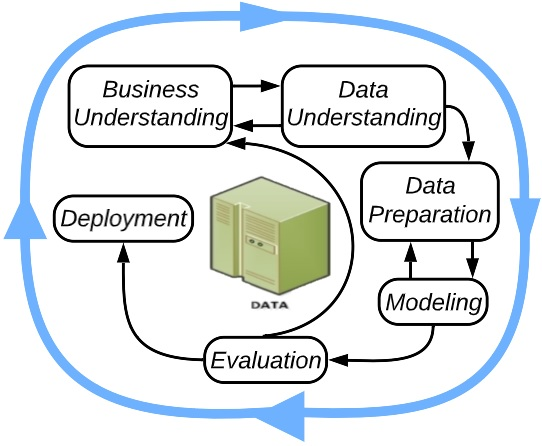
\includegraphics[scale=0.50]{img/ciclocrisp.jpg}
    \caption{Ciclo de Vida de minería de datos. Tomada de \cite{ibmcrisp}.}
    \label{ciclocrisp}
\end{figure}


La metodología CRISP-DM, por sus siglas en Inglés, Cross Industry Standar Process for Data Mining, propone un método probado para orientar trabajos de minería de datos. Puede ser abarcada de 2 maneras; como proceso, ofreciendo un resumen del ciclo vital de la minería de datos; y como una metodología, en la que se incluye descripciones de las fases normales de un proyecto, incluyendo las tareas necesarias de cada etapa y una explicación inter-relacional entre las tareas \cite{ibmcrisp}.\\


Una de las características de esta metodología es su flexibilidad y personalización de un modelo de minería de datos que se adapte a las necesidades del proyecto. Esta metodología cuenta con un ciclo de vida compuesto por 6 fases o etapas no necesariamente secuenciales; y es en estas etapas donde se indican las dependencias más importantes y frecuentes entre las fases \cite{ibmcrisp}.



Tal y como se observa en la figura \ref{ciclocrisp}, las etapas de la metodología son:





\subsection{Business Understanding / Entendimiento del negocio} 
Esta primera etapa consiste principalmente en obtener la máxima cantidad de información posible de los objetivos comerciales. De esta forma se puede identificar de manera clara los objetivos, metas, problemas, y recursos con los que se cuentan para realizar el estudio. La metodología sugiere la recopilación de información sobre la situación comercial actual, los recursos personales, materiales e intangibles. Por otra parte se debe tener claro conocimiento de la estructura de la empresa, patrocinadores internos o externos y unidades comerciales que se verán afectadas positiva o negativamente tras la realización del proyecto de minería de datos \cite{ibmcrisp}.

\subsection{Data Understanding / Entendimiento de los datos}
Esta etapa implica estudiar más de cerca los datos disponibles de minería. Esto es un paso imprescindible para evitar problemas inesperados durante la fase de preparación de datos pues suele ser la más larga en los proyectos \cite{ibmcrisp}.\\

En esta etapa se busca acceder a los datos, explorarlos mediante tablas, gráficos o análisis estadísticos. De esta forma se podrá determinar la calidad de los datos y describir resultados en la documentación del proyecto.

En este punto de la metodología se puede catalogar los datos de 3 maneras distintas
\begin{itemize}
    \item Datos existentes: registros, transacciones, encuesta, registro web, entre otros
    \item Datos adquiridos: Datos adicionales que pueden ser, o no, necesario incluirlos.
    \item Datos adicionales:Datos complementarios si los requiere
\end{itemize}
Con base en lo anterior y con las delimitaciones de la seccion \ref{limites}, se puede establecer que para este proyecto se trabajará principalmente con los datos existentes.

También es importante realizar una descripción detallada de los datos, ya sea en cantidad o calidad; tipos de valores, ya sean numéricos, categóricos o booleanos; esquemas de codificación

\subsection{Data Preparation / Preparación de los datos}
La preparación de datos es uno de los aspectos mas importantes pues se busca que los datos cuenten con una estructura indicada para que los modelos que se propongan pueden satisfacer las necesidades para los que son propuestos. Es posible que para llevar a cabo esta etapa se deba realizar una combinación o agrupación de datos o registros, realizar una selección de muestra de un subconjunto de datos, agregación de registros, clasificación de datos para el modelado, eliminación y/o sustitución de valores en blanco o perdidos, ó la división en conjuntos de datos de prueba, entrenamiento o evaluación \cite{ibmcrisp}.\\

En cuanto a la selección de datos, es necesario que los datos sean relevantes por lo que se pueden seleccionar datos basados en la selección de elementos (filas de registros) o en la selección de atributos (columnas o características). Posteriormente a esto se debe realizar una limpieza de datos en donde se debe tratar con datos perdidos o en blanco, meta datos erróneos o perdidos, incoherencias y errores de datos, en cuyo caso deben ser corregidos \cite{ibmcrisp}.

\subsubsection{Método de ajuste no lineal: Levenberg-Marquardt (LM)}

Si un modelo es lineal en sus parámetros, el objetivo de mínimos cuadrados es cuadrático en los parámetros. Este objetivo puede minimizarse con respecto a los parámetros en un solo paso mediante la solución de una ecuación matricial lineal. Si la función de ajuste no es lineal en sus parámetros, el problema de mínimos cuadrados requiere un algoritmo de solución iterativo. Dichos algoritmos reducen la suma de los cuadrados de los errores entre la función del modelo y los puntos de datos a través de una secuencia de actualizaciones bien elegidas de los valores de los parámetros del modelo \cite{levenberduke}.\\

Siguiendo el método de Gauss-Newton, la suma de los errores al cuadrado se reduce asumiendo que la función de mínimos cuadrados es localmente cuadrática en los parámetros y encontrando el mínimo de esta cuadrática.Esta medida de bondad de ajuste con valores escalares se denomina criterio de error de chi-cuadrado ($\chi^{2}$), porque la suma de los cuadrados de las variables aleatorias normalmente distribuidas se distribuye como la distribución de ($\chi^{2}$). Si la función y es no lineal en los parámetros del modelo, entonces la minimización de con respecto a los parámetros debe realizarse de forma iterativa \cite{levenberduke}. \\

El ajuste de curvas es un proceso que se utiliza para encontrar una función matemática que mejor se ajuste a un conjunto de datos experimentales. Una de las técnicas más populares para el ajuste de curvas es el método de Levenberg-Marquardt, que es una combinación de los métodos de Gauss-Newton y el método del gradiente conjugado \cite{levenberduke}. El método de LM es muy eficiente en la resolución de problemas de ajuste de curvas no lineales, y es ampliamente utilizado en diversas áreas de la ciencia y la ingeniería, incluyendo la física, la química, la biología, la economía y la ingeniería.\\


En términos generales, el método de LM minimiza la función de error cuadrático entre los datos experimentales y el modelo teórico. Este método se basa en un enfoque iterativo que comienza con una estimación inicial de los parámetros de la función de ajuste y se ajusta sucesivamente hasta que se alcanza una solución que minimiza la función de error cuadrático. El método de LM utiliza una matriz jacobiana para calcular la dirección del gradiente y la tasa de aprendizaje de cada paso iterativo. La matriz jacobiana se utiliza para calcular la dirección del gradiente y la tasa de aprendizaje de cada paso iterativo. Si la tasa de aprendizaje es grande, el método funciona como el método del gradiente conjugado. Si la tasa de aprendizaje es pequeña, el método funciona como el método de Gauss-Newton. Por lo tanto, el método de Levenberg-Marquardt es una combinación de ambos métodos \cite{levenberduke}.\\


% \subsubsection{Método de ajuste: Efectos mixtos}
\subsubsection{Método de ajuste no lineal: Efectos mixtos (ME)}

Otro de los métodos de ajuste más utilizados para el análisis individualizado de múltiples objetivos dependientes del tiempo es el ajuste por efectos mixtos lineales y no lineales. Estos modelos de efectos mixtos se basan en un modelo generalizado para describir poblaciones aún cuando los parámetros de crecimiento del modelo pueden ser únicos para los sujetos de estudio \cite{mixedShelley}. En estos modelos, se pueden incorporar tanto efectos fijos como aleatorios, lo que permite tener en cuenta tanto la variabilidad entre individuos como la variabilidad dentro de cada individuo en el tiempo. Para este método, agregar efectos aleatorios a un modelo extiende la confiabilidad de las inferencias más allá de la muestra específica de individuos. \\

Por definición, se puede establecer la respuesta al modelo de efectos mixtos como:

\begin{equation}
    y_{ij} = f(\varphi,x_{ij}) + \varepsilon_{ij}
\end{equation}
\begin{equation}
    \varphi = \beta + b_{i}
\end{equation}

Donde $x_{ij}$, es un vector de predictores, $\varphi$, es un vector de parámetros del modelo, $\varepsilon$, es un error asociado a la medición o al proceso de toma de datos y j es el numero de observaciones existentes en un grupo i. $\varphi$ usualmente es un modelo resultante de la combinación de efectos aleatorios $b_{i}$, que son usualmente descritos como multivariados normalmente distribuidos con media 0. Es importante mencionar que los errores son usualmente asumidos como independientes, idéntica y normalmente distribuidos con varianza constante \cite{matlabmixed}.\\

Los modelos de efectos mixtos tienen en cuenta tanto los efectos fijos como los aleatorios. Así como todos los modelos de regresión, su propósito es describir una variable de respuesta en función de las variables predictoras; sin embargo, los modelos de efectos mixtos reconocen las correlaciones dentro de los subgrupos de muestra. %(no aplicable para este caso pues no los sujetos de estudio son las reses individuales y no hay subgrupos).
De esta manera, proporcionan un compromiso entre ignorar los grupos de datos por completo y ajustar cada grupo con un modelo separado \cite{matlabmixed}. 




\subsection{Modelling / Modelado} 

Este es el punto donde los datos preparados pueden incorporarse a las herramientas analíticas y cuyos resultados podrán arrojar primeros resultados deseados respecto al problema planteado en la comprensión del negocio. El modelado se suele ejecutar en múltiples iteraciones. Normalmente, los analistas de datos ejecutan varios modelos utilizando los parámetros predeterminados y ajustan los parámetros o vuelven a la fase de preparación de datos para las manipulaciones necesarias por su modelo.

Es necesario que el modelo sea acorde a los tipos de datos disponibles, a los objetivos y patrones, y a los requisitos específicos de modelado como por ejemplo si se busca que los resultados sean fácilmente presentables.\\

En cuanto a la generación de los modelos es necesario dedicar el tiempo suficiente para experimentar con distintos modelos antes de llegar a conclusiones definitivas. Estos modelos pueden ofrecer resultados interesantes en cuanto a interpretaciones y conclusiones. También puede realizarse una comparativa de modelos antes de integrarlos o desplegarlos. Para registrar el proceso con una amplia variedad de modelos es necesario asegurarse de registrar los cambios que se realicen en cada modelo en pro de corroborar y/o analizar los resultados cuando sea necesario.

Al final de esta etapa se dispondrá de 3 tipos de información que pueden ser usados para la toma de decisiones posteriores; estos datos son: 
\begin{enumerate}
    \item Configuración de parámetros donde se incluyen las notas que se han tomado sobre los parámetros que ofrecen mejores resultados.
    \item Los modelos producidos.
    \item Las descripciones de resultados de los modelos, incluyendo resultados asociados a problemas con los datos, rendimiento y exploración de resultados
\end{enumerate}

\subsubsection{Modelamiento por Ecuaciones Diferenciales Ordinarias (EDOs)}
\subsubsection{Modelamiento EDO: Balance de energía}


\subsection{Evaluation and Assesment / Evaluación} 

En este punto, se habrá completado la mayor parte del proyecto. También se habrá determinado, en la fase de modelado, que los modelos son técnicamente correctos y efectivos en función de los objetivos que se han definido previamente. Esta etapa de la metodología produce 2 tipos de resultados: \begin{itemize}
    \item Los modelos finales seleccionados en la fase anterior de CRISP-DM.
    \item Las conclusiones o interferencias obtenidas de los modelos y del proceso de minería de datos; recibiendo el nombre de \textit{\textbf{descubrimientos}}.
\end{itemize}

Es en esta etapa donde se debe verificar si los resultados se expresan con claridad y de forma que se pueden representar con facilidad; si se han realizado descubrimientos especiales o particularidades que se deban resaltar; y si los resultados se adaptan a los objetivos del proyecto. Una vez haya evaluado los resultados, es recomendable realizar una lista de el (los) modelo(s) aprobado(s) para incluir en el informe final.


\subsection{Deployment / Despliegue} 
En general, la fase de despliegue de CRISP-DM incluye dos tipos de actividades:
\begin{itemize}
    \item Planificación y control del despliegue de los resultados
    \item Finalización de tareas de presentación como la producción de un informe final y la revisión del proyecto
\end{itemize}


\chapter{Visión global del contexto \\ ganadero multipropósito} \label{visglob}
%%%%%%%%%%%%%%%%%%%%%%
% DESCRIPCION DEL PROBLEMA
%%%%%%%%%%%%%%%%%%%%%%

En este capítulo se describe parte del contexto ganadero actual de cárnicos en Colombia y el Cauca y algunas de las características principales relacionadas al proceso de ceba en ganado vacuno. Estos temas sirven como base conceptual para comprender el análisis y diseño empleados en este proyecto.

%En este capitulo se explica el contexto ganadero actual y algunas de las características principales relacionadas al proceso de ceba.(Esto estaba antes del 15 de Agsoto de 2019 que hice los cambios en bOSCH)

%El titulo debe ser algo como Contexto general de la ganaderia de carne

%Tengo que agregar algo como otro capitulo de solo lo del tornillo (creo que alcanza) o sino agregarlo a lo de ELECTRÜONICA EN EL AGRO y combinar ese capitulo y PONERLE OTRO NOMBRE.


\section{Generalidades agropecuarias} \label{tgan}
%\section{Visión global} \label{tgan}
%\section{Contexto ganadero en Colombia} \label{tgan}

%ESTO SE BORRA-> Explicar el CONTEXTO, síntomas y causas del problema a resolver. (1.5 páginas).EXPLICAR QUE VOY A HACER \\ \\

La fortaleza principal del sector primario colombiano radica en la producción de recursos de la naturaleza. Esto se refiere a las actividades económicas en relación a los procesos de producción en el sector agropecuario. Este sector abarca el conjunto de técnicas y las acciones que permiten trabajar y cultivar la tierra para producir materias primas así como también la producción de recursos de la ganadería.

Por su parte, el sector ganadero alude a los diferentes tipos de ganado de una zona y a las actividades que se emplean para criar y comercializar a estos animales y a los productos derivados de estos. En Colombia se practican diferentes modalidades de ganadería con base en el tipo de ganado de enfoque tales como:

\begin{itemize}
\item Bovinos ó Vacunos
\item Equinos
\item Mulares y asnales
\item Ovinos
\item Porcinos
\end{itemize}

De igual forma, estos tipos de ganado son trabajados con diferentes designaciones, entre las cuales se pueden mencionar:

\begin{itemize}
\item Crianza y material reproductivo: Tiene como objetivo la reproducción de ganado mediante el cruce de individuos con las mejores características biológicas para mejorar así la genética de los individuos. Los mejores ejemplares son comercializados como material reproductivo y producción de leche dependiendo de su sexo (macho y hembra respectivamente), y los demás ejemplares pasan a ser parte de la ganadería de la carne.
\item Producción de leche y derivados lácteos: Como su nombre lo indica, es el ganado designado para la producción cuantitativa y cualitativa de leche mediante ordeño manual, mecánico o eléctrico.
\item Producción de carne: Encaminado a la producción cuantitativa y cualitativa de carne.
\end{itemize}

\subsection{Caracteres zootécnicos del ganado vacuno}

La destinación del ganado vacuno para producción de leche, material reproductivo o engorde depende de algunos factores fisonómicos y biológicos. Por ello se hace mención de estos atributos a continuación:

\begin{figure}[H]
 \begin{center}
 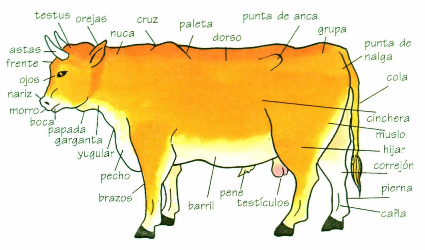
\includegraphics[scale=0.9]{img/dibujito1.png}
 \end{center}
 \caption{Partes físicas de un bovino. Tomada de \cite{librito1}}
\end{figure}

%%% Tek: faltan lsa refs para las figs

\subsubsection{Clasificación vacuna por aptitud productiva}
\begin{itemize}
\item \textbf{Lechero:} (Cabe resaltar que un requerimiento o propiedad fisonómica básica es que posean ubre, esto quiere decir solo las hembras pueden hacer parte de esta aptitud productiva). Poseen formación triangular, cuentan con cuerpo y extremidades largas y delgadas con poca voluminosidad cárnica
\begin{figure}[H]
 \begin{center}
 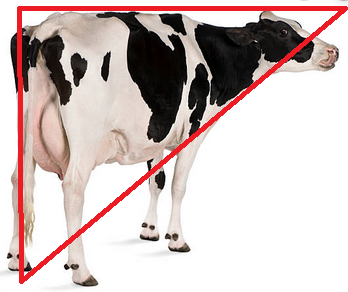
\includegraphics[scale=0.9]{img/dibujito2.png}
 \end{center}
 \caption{Aptitud lechera. Tomada de \cite{googlepics}. }
\end{figure}
\item \textbf{Carne:} Poseen una contextura rectangular. Además de poseer un cuerpo ancho con sus extremidades bien dotadas de carne.
\begin{figure}[H]
 \begin{center}
 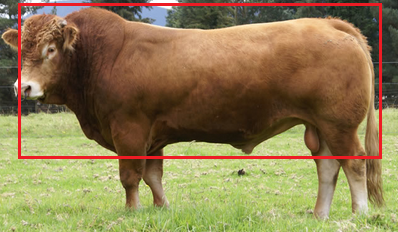
\includegraphics[scale=0.9]{img/dibujito3.png}
 \end{center}
 \caption{Aptitud de tipo carne. Tomada de \cite{googlepics}. }
\end{figure}
\item \textbf{Doble propósito:} Cuentan con propiedades mixtas de los 2 tipos ya mencionados, por lo que tanto su contextura, como volumen cárnico, ubre y extremidades son medianas. Este tipo de animales poseen una mayor facilidad en la adaptación del clima, alimentación y manejo. 
\begin{figure}[H]
 \begin{center}
 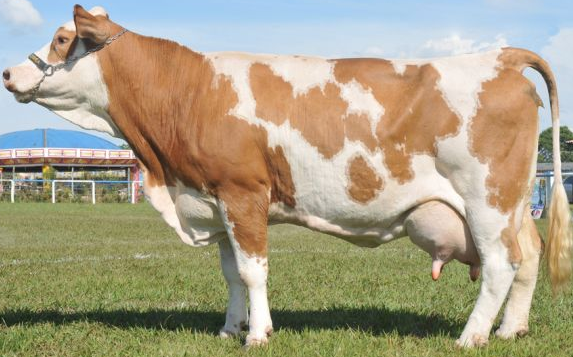
\includegraphics[scale=0.8]{img/dibujito4.png}
 \end{center}
 \caption{Aptitud de doble propósito.  Tomada de \cite{googlepics}. \label{}}
\end{figure}
\end{itemize}

% A modo general y para el desarrollo de este trabajo desde este punto en adelante, se decide describir más a fondo el ganado vacuno y enfocarse en describir de manera más profunda las ganaderías de la carne y la leche.\\


En el Cauca, aunque se cuente con abundantes hectáreas de diferentes fertilidades y condiciones térmicas apropiadas para el cultivo y desarrollo de la ganadería, se presentan muchas falencias en materia tecnológica y económica, en donde los movimientos migratorios de campesinos desplazados y los efectos colaterales del conflicto armado que se ha presentado en el país, son las principales causas de estas falencias. Sin embargo, el emprendimiento de los pequeños y medianos productores da paso a nuevas oportunidades de intervención por parte de la ingeniería electrónica y el manejo aplicativo de nuevas tecnologías que permitan tener un contacto más cercano con la población campesina.\\



Lo anterior se diseña y se plantea acorde con el manual de Buenas Prácticas de Ganadería  (BPG) y con las legislaciones pertinentes al manejo de alimentos para el consumo humano establecidas por la ley colombiana mencionados en la sección \ref{leyes}.

%%%%%%%%%%%%%%%%%%

\section{Sistemas de explotación del ganado vacuno}

Indiferentemente de su aptitud productiva, el ganado vacuno debe situarse en una infraestructura o ambiente apropiado para su desarrollo. Sin embargo, por  cuestiones geográficas, geológicas y/o climatológicas, los animales son criados mediante métodos de explotación como el estabulado, semiestabulado y el silvopastoril:\\

\begin{figure}[H]
 \begin{center}
 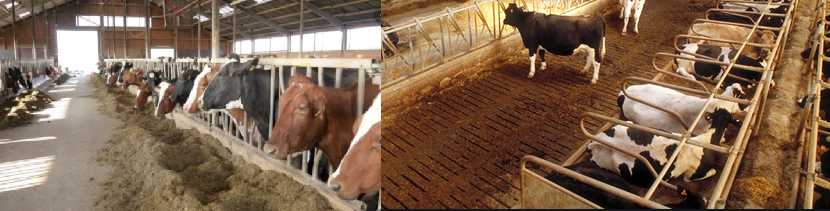
\includegraphics[scale=0.8]{img/estabulado.png}
 \end{center}
 \caption{Sistema de explotación estabulada. Tomada de \cite{googlepics}. \label{estabulpng}}
\end{figure}

El sistema ``estabulado'' (Ver figura \ref{estabulpng}) es una forma de crianza de ganado en la cual los animales pasan la mayor parte del tiempo en establos donde realizan sus actividades diarias. En estos establos se recrea la vida del ganado con la diferencia que el mismo se encuentra protegido bajo techo sin tener exposición directa al sol y a las condiciones medio ambientales. En este sistema se pretende una mayor producción y mejor calidad de la carne en el menor tiempo posible \cite{defestabulacion}.\\

 Por su parte el sistema ``silvopastoril' (ver Figura \ref{silvopng})' es una forma de cultivo agropecuario que involucra la presencia de árboles interactuando con gramíneas y los animales sometidos a un manejo determinado para incrementar la productividad y el beneficio neto de la explotación a mediano y corto plazo \cite{defsilvopas}.

\begin{figure}[H]
 \begin{center}
 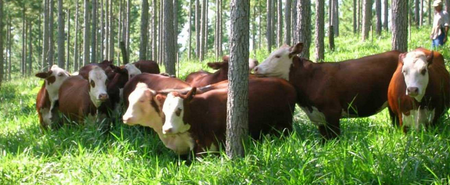
\includegraphics[scale=0.9]{img/silvopastoril.png}
 \end{center}
 \caption{Sistema de explotación silvopastoril. Tomada de \cite{contextoganadero}. \label{silvopng}}
\end{figure}

Finalmente, en el sistema semiestabulado se combinan los 2 sistemas mencionados. En este sistema mixto, los animales ingieren sus raciones de alimento principal en áreas extensas de pastos y forrajes vegetales, mientras que el cuidado y el suministro especializado de vitaminas y proteínas se realiza bajo techo.
%\begin{figure}[H]
% \begin{center}
% \includegraphics[scale=0.6]{img/tiposdosif.png}
% \end{center}
% \caption{Sistema de explotación por estabulación.  \label{estabulpng}}
%\end{figure}
%\begin{figure}[H]
% \begin{center}
% \includegraphics[scale=0.6]{img/tiposdosif.png}
% \end{center}
% \caption{Sistema de explotación silvopastoril. \label{silvopng}}
%\end{figure}
\subsection{Ciclo productivo de la leche}

% 2/10/2022 Cambiar la iamgen por una que tenga que ver con leche y luego descomentar el begin figure 
% \begin{figure}[H]
% \begin{center}
% 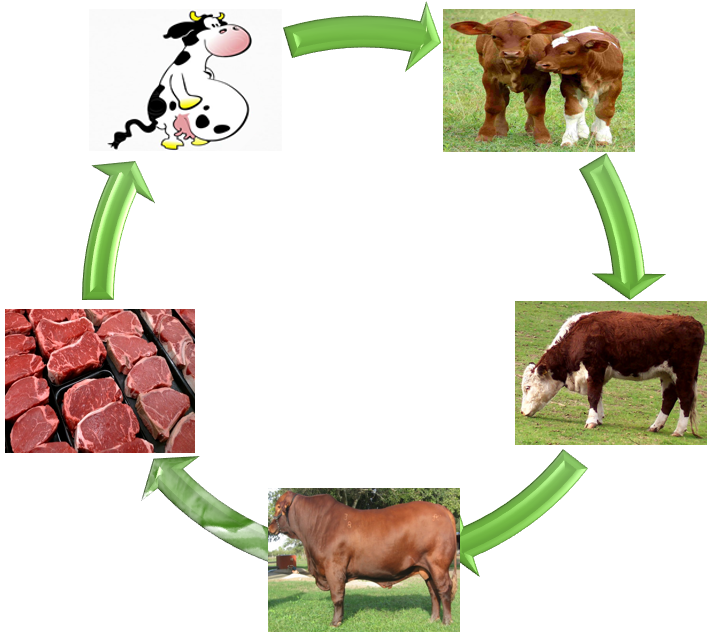
\includegraphics[scale=0.45]{img/ganadcarne.png}
% \end{center}
% \caption{Ciclo productivo en la ganadería de ordeño. \label{ganadcarnepng}}
% \end{figure}

% (Ver Figura \ref{ganadcarnepng}) 
 
El ciclo productivo de la leche de un ganado destinado para tal fin consta de 3 etapas principales que abarcan desde la gestación de la cría y maxima producción de leche, seguido de un periodo de declive y persistencia de producción y finalizando con el periodo de secado en donde se da descanso a la vaca para que se regenere el tejido glandular productor de leche para la siguiente lactancia \cite{mahecha}.\\

Estas etapas son brevemente descritas a continuación:


% \begin{itemize}
    \subsubsection{Etapa de crianza:} Es la etapa de producción temprana en donde el animal (generalmente crías hembras denominadas terneras) son alimentadas y criadas hasta alcanzar 2 años de edad.
	\begin{itemize}
% 		\item En esta etapa se requiere de grandes extensiones de tierra para producir crías
		\item No requiere de estaciones climatológicas específicas y se puede dar en todo el año (Esta característica varía dependiendo de la ubicación geográfica y las exposiciones climatológicas).
		\item Los elementos principales en la dieta de estas criaturas son los nutrientes provenientes del Calostro, la leche materna, forraje y vitaminas.\\
	\end{itemize} 
	\subsubsection{Etapa de gestación y ordeño:} Es la etapa inmediatamente siguiente a la etapa de crianza, en donde la novilla esta desarrollada y en la capacidad de ser inseminada para iniciar su producción de leche.
	\begin{itemize}
% 		\item En esta etapa se estima que el peso del animal puede alcanzar un mínimo de 230[kg] de peso en adelante.
% 		\item Es considerada como la etapa más rentable debido a las  pocas exigencias en materia de calidad alimenticia. 
		\item El objetivo de esta etapa es que la novilla produzca leche mientras que se da la gestación del novillo dentro de ella.
		\item El alimento se basa en pasturas de calidad, provenientes de las extensiones de tierra donde comen las reses y se crían.
		\item El animal gana mayor peso debido a su etapa de crecimiento, por lo que entre mejor sea su alimentación se obtendrán mejores resultados.
		\item Es de vital importancia que el animal se encuentre en la capacidad de  alimentarse \texit{Ad Libitum}, es decir a placer y a voluntad.
		\item En esta etapa, la novilla es denominada primípara, pues se encuentra abarcando el tiempo de gestación de su primera cría.\\
	\end{itemize} 
	\subsubsection{Etapa seca o de secado:} Es la etapa final que abarca los últimos 2 meses de gestación previos al parto en donde se da paso a la regeneración de tejidos glandulares que producen leche y a la curación de las glándulas mamarías para reducir el riesgo de mastitis. En sus características principales se pueden mencionar:
	\begin{itemize}
		\item Aún cuando la novilla primípara esta en capacidad de producir leche, no se debe recurrir al ordeño hasta que no se realice el parto.
	\end{itemize}
% \end{itemize} 

\subsubsection{Razas}

Debido a la gran variedad de especies, condiciones ambientales, y al proceso evolutivo del ganado, históricamente se ha podido clasificar y seleccionar las razas más representativas para este tipo de explotación ganadera. Más precisamente se puede hacer mención de las siguientes:
\begin{multicols}{2}
    \begin{center}
        \begin{itemize}
        \item Simmental
        \item Holstein
        \item Jersey
        \item Normando
        \end{itemize}
    \end{center}
\end{multicols}

Éstas son seleccionadas principalmente por la contextura voluminosa pero factores como la calidad de la leche pueden sobrepasar los criterios cuantitativos. A continuación se muestran algunos ejemplares de estas razas:

\begin{figure}[H]
 \begin{center}
 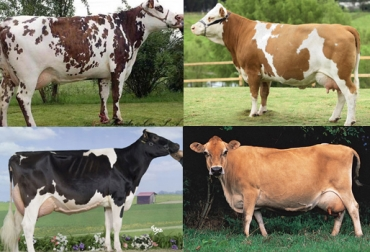
\includegraphics[scale=1]{img/razaslecheras.png}
% \end{center}
 \caption{En la primer fila de izquierda a derecha se observan ejemplares de las razas Normando, Simmental; seguido de las razas Holstein y Jersey en la fila inferior. Tomada de \cite{contextoganadero} \label{cuadrorazaspng}}
  \end{center}
\end{figure}

\subsection{Ciclo productivo de la carne}

\begin{figure}[H]
\begin{center}
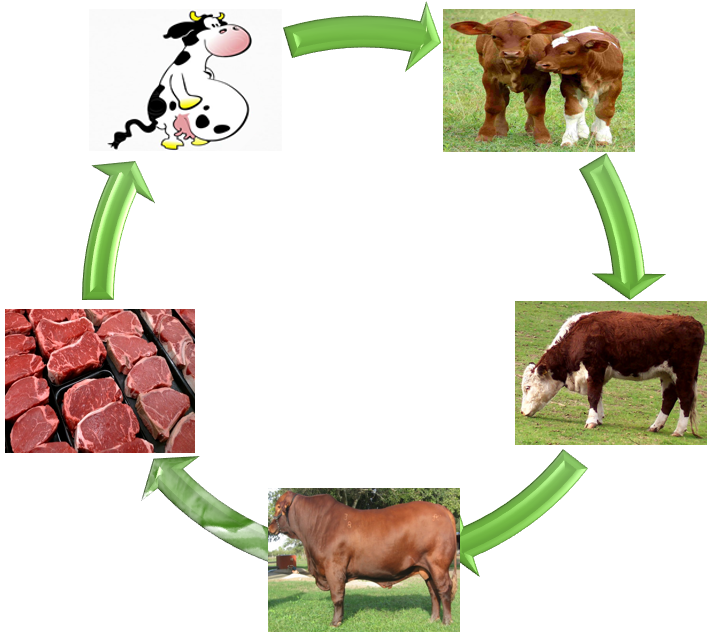
\includegraphics[scale=0.55]{img/ganadcarne.png}
\end{center}
\caption{Ciclo productivo en la ganadería de la carne.  Tomada de \cite{contextoganadero}. \label{ganadcarnepng}}
\end{figure}

 
El ciclo productivo de la carne (Ver Figura \ref{ganadcarnepng})  de un ganado destinado para tal fin consta de 3 etapas principales que abarcan desde el nacimiento de la cría, su desarrollo y crecimiento y finalizando con su comercialización en el momento en que alcanza las condiciones apropiadas para ser transformado en carne para consumo humano \cite{mahecha}. Estas etapas son brevemente descritas a continuación:


%y finalizando en el momento en que alacanza las condiciones apropiadas para ser transformado en carne para consumo humano \cite{mahecha}. Estas etapas son brevemente descritas a continuación:

\begin{itemize}
	\item \textbf{Ganadería de Cría:} Es la etapa de producción temprana en donde el animal (generalmente crías macho llamadas bovinos) es alimentado y criado desde su nacimiento hasta los primeros seis (6) meses de edad. 
	\begin{itemize}
		\item En esta etapa se requiere de grandes extensiones de tierra para producir crías
		\item No requiere de estaciones climatológicas específicas y se puede dar en todo el año.
		\item Los elementos principales en la dieta de estas criaturas son los nutrientes provenientes del Calostro y la leche materna.\\
	\end{itemize} 
	\item \textbf{Ganadería de Levante:} Es la etapa inmediatamente siguiente a la etapa de crianza, en donde el bovino se desarrollará entre los siete (7) y diez y ocho (18) meses de edad.
	\begin{itemize}
		\item En esta etapa se estima que el peso del animal puede alcanzar un mínimo de 230[kg] de peso en adelante.
		\item Es considerada como la etapa más rentable debido a las  pocas exigencias en materia de calidad alimenticia. 
		\item El objetivo de esta etapa es que el sujeto en cuestión alcance el peso deseado en el menor tiempo posible con el menor esfuerzo posible
		\item El alimento se basa en pasturas de calidad, provenientes de las extensiones de tierra donde comen las reses y se crían.
		\item El animal gana mayor peso debido a su etapa de crecimiento, por lo que entre mejor sea su alimentación se obtendrán mejores resultados.
		\item Es de vital importancia que el animal se encuentre en la capacidad de  alimentarse \texit{Ad Libitum}, es decir a placer y a voluntad.\\
	\end{itemize} 
	\item \textbf{Ganadería de engorde o Ceba:} Es la etapa final que abarca desde los 19 meses de edad hasta los 24 o 36 meses, dependiendo de su crecimiento  y otros factores como el interés del productor, la demanda del mercado, entre otras. En sus características principales se pueden mencionar:
	\begin{itemize}
		\item El límite se define por los intereses del productor, la demanda del mercado y en general por el peso ideal del animal que es aproximadamente mayor o igual a los 450[kg].
		\item Para la alimentación se requieren de buenas, grandes y controladas cantidades con el fin de mejorar la carne. Para esto se utilizan dietas que requieren pasturas y concentrados dietarios.
		\item Se debe monitorear la alimentación tomando registro en la ganancia de gramaje diaria de cada uno de los animales.
	\end{itemize}
\end{itemize} 

\subsubsection{Razas} Debido a la gran variedad de especies, condiciones ambientales, y al proceso evolutivo del ganado, históricamente se ha podido clasificar y seleccionar las razas más representativas para este tipo de explotación ganadera. Más precisamente se puede hacer mención de las siguientes:
\begin{multicols}{2}
\begin{center}
\begin{itemize}
\item Beefmaster
\item Charolais
\item Simmental
\item Angus
\item Brangus
\item Santa Gertrudis
\item Hereford
\item Limousin
\item Cebú
\item Belgina Blue
\end{itemize}
\end{center}
\end{multicols}

Éstas son seleccionadas principalmente por la contextura voluminosa pero factores como la calidad de la carne pueden sobrepasar los criterios cuantitativos. A continuación se muestran algunas de las razas más usadas para este propósito:

\begin{figure}[H]
 \begin{center}
 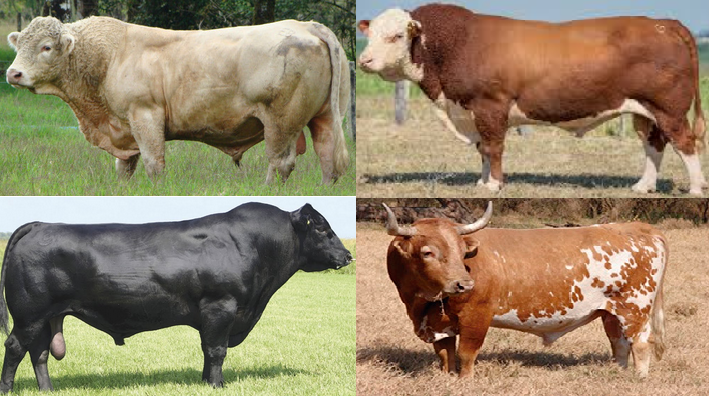
\includegraphics[scale=0.8]{img/cuadrorazas.png}
% \end{center}
 \caption{En la primer fila de izquierda a derecha se observan ejemplares de las razas Charolais, Hereford; seguido de las razas Angus y Criolla en la fila inferior.  Tomada de \cite{contextoganadero}. \label{cuadrorazaspng}}
  \end{center}
\end{figure}


\subsection{Alimentación y Componentes básicos de la dieta}
%\section{Marco de referencia}
% \subsubsection{Alimentación}
La alimentación de un cultivo de ganado requiere de una dieta o ración con diferentes componentes básicos o nutrientes que deben ser suministrados día a día de forma balanceada para lograr un crecimiento óptimo y que los animales puedan expresar su potencial genético \cite{recomendaciones}.\\

Los componentes principales que conforman la dieta alimenticia  del ganado son:
% 	\begin{itemize}
	

\subsubsection{Agua}
    Componente principal de la alimentación. Esta debe ser suministrada en cantidad y calidad para ser aprovechada por cada animal llegando a ocupar más del 50\% de la masa corporal de un ejemplar adulto y hasta un 90 \% de un recién nacido.
    	
	\begin{figure}[H]
	 \begin{center}
	 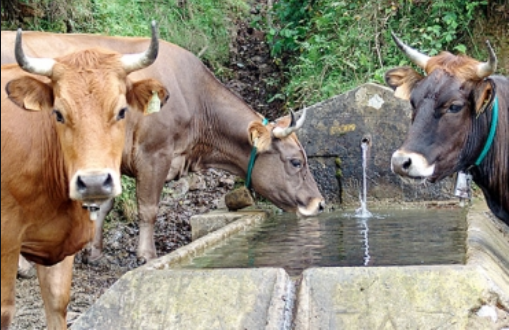
\includegraphics[scale=0.8]{img/agua.png}
	 \end{center}
	 \caption{Hidratación del ganado. Tomada de \cite{contextoganadero}.	\label{energeticospng}}
	\end{figure}
    	
\subsection{Energía}
Este componente se suministra mediante azúcares, almidones, celulosa, entre otros, los cuales aportan grandes cantidades de energía mas no de proteína, razón por la cual se deben suministrar de forma complementaria.
	\begin{figure}[H]
	 \begin{center}
	 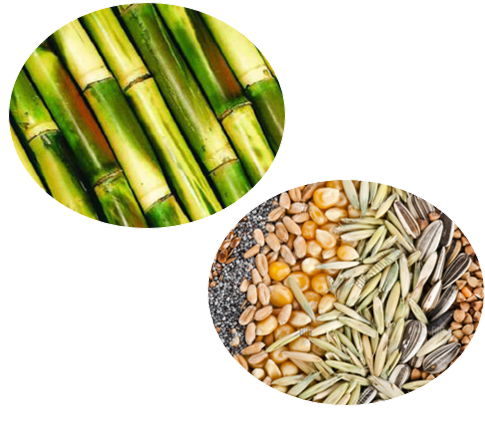
\includegraphics[scale=0.7]{img/melazacana.png}
	 \end{center}
	 \caption{Suplementos energéticos. 	\label{energeticospng}}
	\end{figure}
    
\subsection{Proteínas}
Estos nutrientes son fundamentales especialmente durante los periodos de sequía, por consiguiente, se optan por fuentes altas en proteína como leguminosas forrajeras, el Maní, Leucaena y el más común, los pastos de forraje verde. 
	\begin{figure}[H]
	 \begin{center}
	 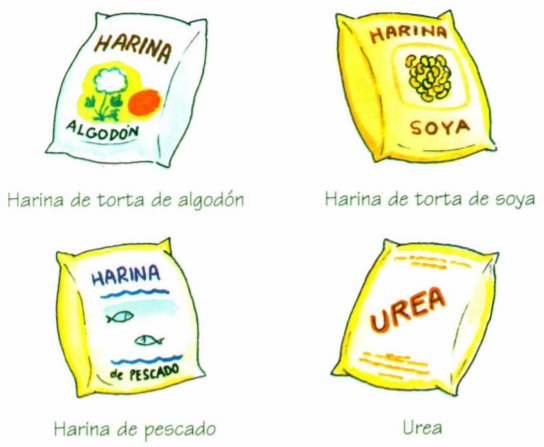
\includegraphics[scale=0.8]{img/proteina.png}
	 \end{center}
	 \caption{Suplementos proteínicos. Tomada de \cite{librito1}. \label{proteinaspng}}
	\end{figure}

\subsection{Minerales}
Son indispensables en la ganancia de peso de los novillos durante la etapa de Cría y Levante. Este complemento alimenticio debe estar siempre a la disposición para que el ganado pueda abastecer sus necesidades. Estos minerales se suelen proporcionar mediante mezclas de macrominerales y microminerales que se ofrecen de libre consumo al ganado.

\subsection{Vitaminas}
Suministradas en cantidades pequeñas aplicadas comúnmente en animales cuya alimentación se basa en forrajes secos,  o en animales enfermos convalecientes, desnutridos o durante épocas de sequía prolongada.
	\begin{figure}[H]
	 \begin{center}
	 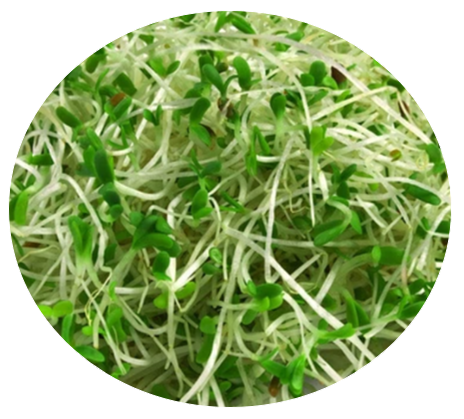
\includegraphics[scale=0.6]{img/leguminosas.png}
	 \end{center}
	 \caption{Forraje y leguminosas. Tomada de \cite{librito1}. \label{vitaminaspng}}
	\end{figure}

\subsection{Balance de raciones y dietas especializadas}
% \subsubsection{Balance de raciones y dietas especializadas}
    Estas dietas son suministradas por personal técnico calificado que prepara un dieta acorde a la cantidad de nutrientes de cada animal de forma particular e independiente, considerando su peso actual, su velocidad de crecimiento y estado fisiológico.

\subsection{Desperdicios}

\section{Leyes y Normatividad}  \label{leyes}
Requerida para que el avance ganadero se realice de manera coordinada o estandarizada basada en las buenas prácticas ganaderas en pro de mejorar la productividad y ayudarla a alcanzar niveles de ganadería bovina del mundo \cite{invima}, \cite{leylacteos}, \cite{minsaludleche}. 
\begin{itemize}
	\item \textbf{Resolución 2310 de 1986:} Reglamentación parcial en el titulo V de la ley 09 de 1979 que se refiere al procesamiento, composición, requisitos, transporte, y comercialización de los Derivados Lácteos.
	\item \textbf{Resolución 11961 de 1989:} Reglamentación parcial a la resolución 2310 de 1986 que se refiere a lo relacionado con las clases de leche fermentada.
	\item \textbf{Decreto 0616 de 2006:} Reglamento técnico sobre los requisitos que debe cumplir la leche para el consumo humano que se obtenga, procese, envase, transporte, comercialice, expenda, importe o exporte en el país.
	\item \textbf{Resolución 0012 de 2007:} Por la cual se establece el sistema de pago de la leche cruda al productor, diseñado por la Unidad de Seguimiento de Precios.
	\item \textbf{Decreto 1500 de 2007:} Reglamento técnico a través del cual se crea el Sistema Oficial de Inspección, Vigilancia y Control de la Carne y otros productos comestibles y derivados cárnicos destinados para el consumo humano.
	\item \textbf{Decreto 072 de 2007:} Por el cual se establece el manual de buenas prácticas de manejo para la producción de ganado bovino.
	\item \textbf{Decreto 2905 de 2007:} Por el cual se establece el reglamento técnico sobre los requisitos sanitarios y de inocuidad de la carne y productos cárnicos comestibles de las especies bovina y bufalina destinados para el consumo humano.
	\item \textbf{Decreto 18119 de 2007:} Por el cual se reglamenta los requisitos del plan gradual de cumplimiento para  las plantas de beneficio y desposte de bovino y bufalinos.
	\item \textbf{Decreto 2278 de 1982:} Reglamentación parcial en el titulo V de la ley 09 de 1979 que se refiere al sacrificio de animales de abasto público o para consumo humano y el procesamiento, transporte y comercialización de su carne.

\end{itemize}

% \section{Conceptos adicionales}
% \item \textbf{Jáquima:} Es un freno, cabestro o cabezada usado en la ganadería principalmente equina, para identificar, amansar o manipular al animal \cite{jaquima}.

% %%%%%Productos y resultados que se entregarán cuando finalice el proyecto (1/2 página). 


\chapter{CRISP - DM: ETAPA \#1 \\ Entendimiento del negocio}
\label{crisp1}
% A continuación se describen los participantes del modelo de negocio que influyen en la producción ganadera del CA-SENA-POP:

\section{Servicio Nacional de Aprendizaje (SENA)}

El SENA es un establecimiento público de educación en Colombia que ofrece formación gratuita con programas técnicos, tecnológicos y complementarios; que busca la incorporación y el desarrollo de las personas en actividades productivas que contribuyan al desarrollo social, económico y tecnológico del país. Entre las diferentes áreas de formación ofrecidas por el SENA, se encuentra el área de las ciencias agropecuarias, siendo esta la que tiene mayor influencia en la institución.\cite{sena}


\subsection{Centro Agropecuario}

El centro agropecuario (CA) tiene como objetivo liderar la formación de los sub-sectores agrícola, pecuario, pesquero y forestal de la región; mediante alianzas estratégicas con agremiaciones, administraciones municipales, campesinas y centros de educación técnica, media y superior. El CA incorpora tecnologías alternativas en las explotaciones agropecuarias para mejorar la calidad de los productos, reduciendo a su vez costos de producción. Dentro de los servicios ofertados por el CA-SENA se encuentran la producción y comercialización bovina y bufalina, procesamiento de alimentos y control de calidad (Cárnicos y Lácteos), entre otros\cite{casena}.

\section{Empresa donde se realiza el estudio: CA-SENA-POP}

El CA-SENA seccional Cauca, se encuentra ubicado en el norte de la ciudad de Popayán. Cuenta con una granja de aproximadamente 6 hectareas en las que realizan sus actividades productoras con unidades de producción bovina, porcina, avícola, bufalina, caprina, entre otras. Su formación y capacitación consta en gran medida de las prácticas realizadas por los aprendices en cada una de las unidades productoras.La granja se encuentra dividida en 2 zonas, el área usada para las instalaciones de la seccional Popayán y los lotes donde se realizan las diferentes prácticas y servicios mencionados con anterioridad.\\

Se cuenta con un total de 50 lotes de aproximadamente $500m^{2}$ cada uno (ver figura \ref{potrerosenapng}). 30 de ellos son usados para la producción silvopastoril bovina, 10 de ellos son usados para la producción de frutas, hierbas y hortalizas, entre ellas el botón de oro que es usado como forraje complementario en la dieta del ganado vacuno; y los lotes restantes son usados por las otras unidades productoras. Enfocándonos hacia la producción bovina, el CA-SENA-POP, se dedica a explotación del ganado vacuno con fines de producción lechera. Tal y como se ha mencionado antes, manejan un sistema de explotación silvopastoril semiestabulado, dado que distribuyen a sus animales en los diferentes lotes destinados para tal fin y llevan el registro de las cantidades de alimento concentrado y dietas secas, en un establo donde dosifican las cantidades correspondientes de sales minerales y proteínas concentradas.\\

\begin{figure}[H]
	 \begin{center}
	 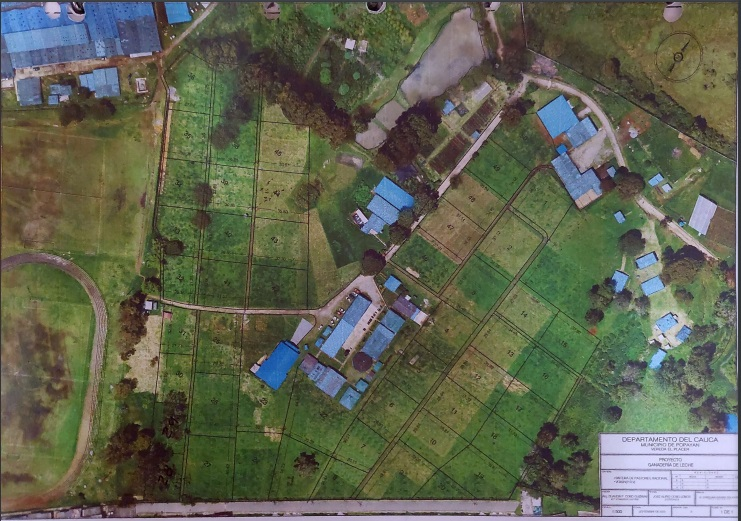
\includegraphics[scale=0.675]{img/potrerosena.jpg}
	 \end{center}
	 \caption{Granja del CA-SENA-POP. \label{potrerosenapng}}
	\end{figure}
	
\section{Negocio y comercialización de productos}

El CA-SENA-POP, realiza la venta de productos ganaderos entre los que se puede mencionar, la producción de leche cruda, reses productoras de leche y terneros para engorde. El CA-SENA-POP ha manifestado que los precios de compra y venta son los precios manejados en el mercado tanto por kg de peso del animal como por kilogramo de leche producida.\\


En el capítulo siguiente, se realiza una descripción de los datos presentes en el CA-SENA-POP usados para este proyecto de investigación




\chapter{CRISP - DM: ETAPA \#2 \\ Entendimiento de los datos}
\label{crisp2}

\section{Adquisición de datos}
\subsection{Registros de ``Leche''}
En el establo de alimentación y dosificación de concentrado, es donde se realizan las tareas de ordeño para las vacas que aportan a la producción neta de leche. El ordeño y la extracción de la leche se ha realizado de manera manual desde sus inicios, pero cuentan con sistemas de ordeño mecánico desde los últimos años. El pesaje de la leche se realiza en kilogramos y el registro de los datos de producción lechera se ha realizado de manera manual en diarios históricos de producción neta. Un ejemplar de estos diarios puede observarse a continuación en la Figura \ref{regleche1png}:

\begin{figure}[H]
	 \begin{center}
	 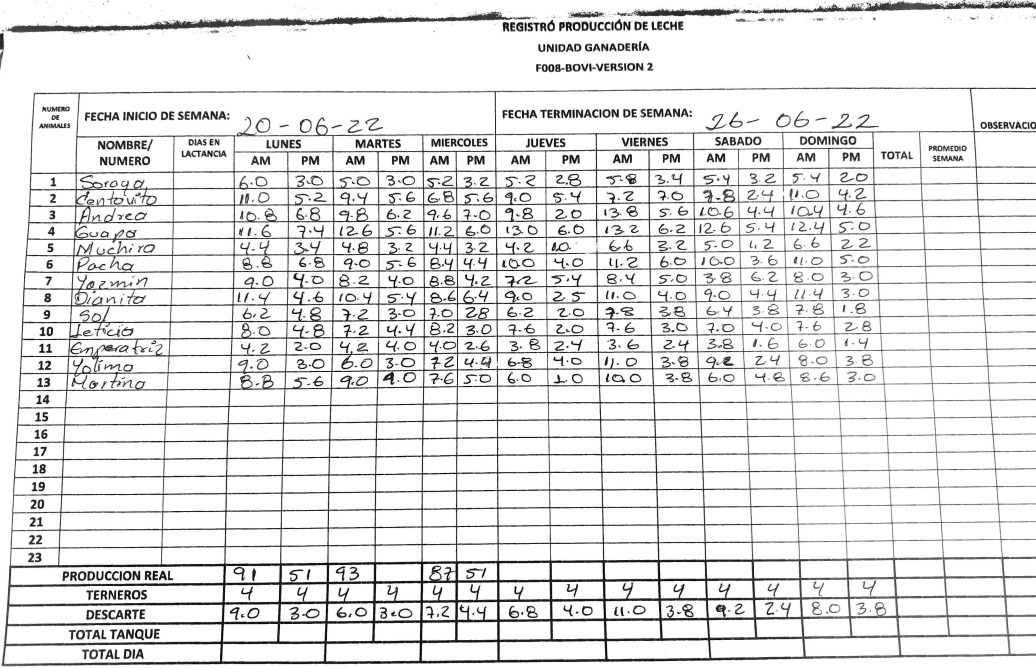
\includegraphics[scale=0.515]{img/regleche1.jpg}
	 \end{center}
	 \caption{Registros manuales de producción lechera en el CA-SENA-POP. \label{regleche1png}}
	\end{figure}
	
Tal y como se puede observar, se lleva un registro diario de cada una de las vacas que se encuentran en etapa de ordeño. Los ordeños se realizan en 2 franjas horarias, en las mañanas, aproximadamente a las 6:00 am, que se realiza el ordeño matutino; y en las tardes, aproximadamente a las 4:00 pm, que se realiza el ordeño vespertino. El registro de los datos se realiza en hojas cuadriculadas donde se puede evidenciar, la producción diaria de cada animal, así como también la producción diaria neta de la unidad de ganadería. Los datos aquí registrados también permiten observar si hay leche que ha sido suministrada a los terneros o si ha sido descartada por sospecha de mastitis, entre otros motivos. \\
	
Aún cuando se lleva un registro manual de los datos, en los últimos 5 años se dio inicio a una migración de datos de manera tecnológica, mediante licencias de software de pago para manejo de producciones ganaderas, entre ellas la licencia del software ``TaurusWebs'' (ver Figura \ref{tauruspng}). Sin embargo, esta transición tecnológica no ha sido implementada en su totalidad, por lo que el registro de datos, se realiza de ambas formas en pro de que los datos no se pierdan. Por otra parte, el manejo de datos manual es utilizado para que sirva de material de estudio y aprendizaje en las diferentes actividades y servicios ofrecidos por el SENA, tales como los cursos de formación y capacitación de ganadería.

\begin{figure}[H]
	 \begin{center}
	 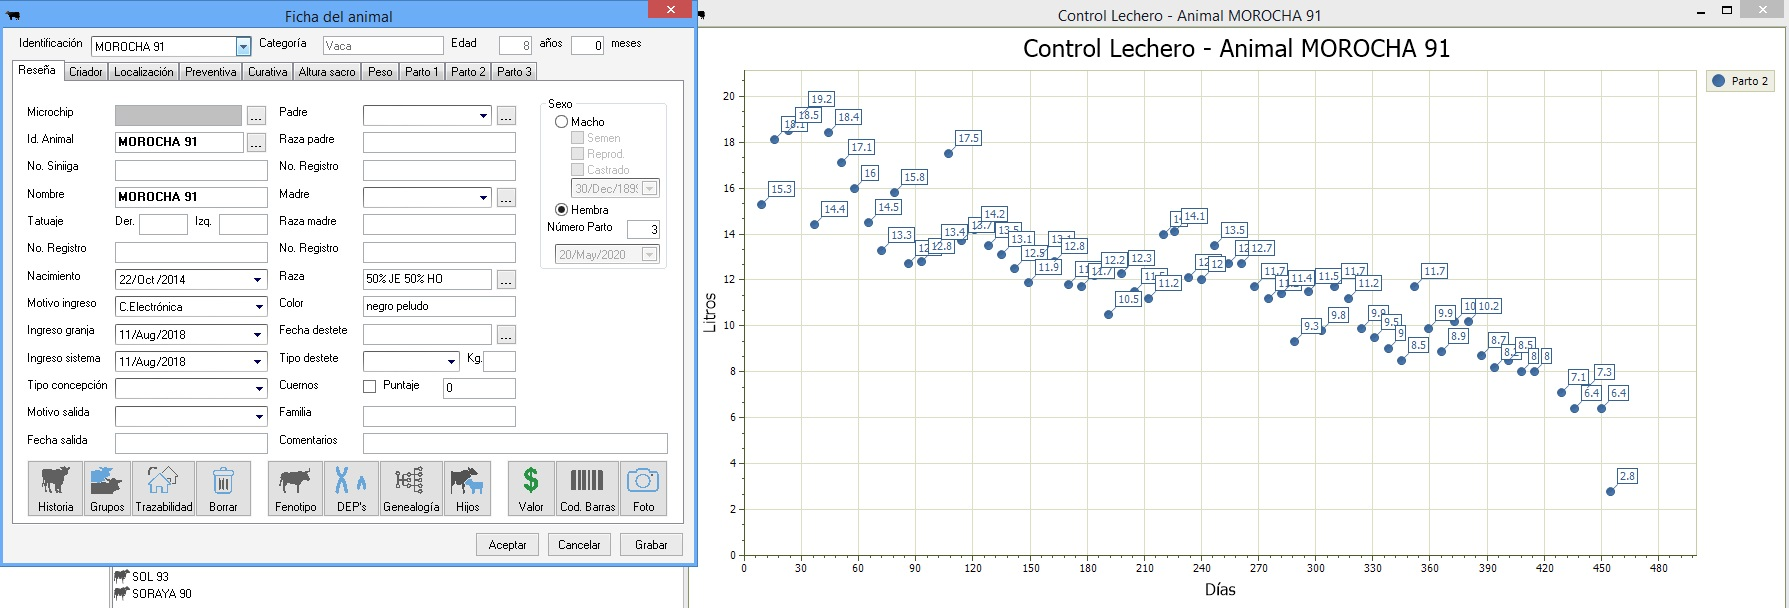
\includegraphics[scale=0.345]{img/ejtaurus.jpg}
	 \end{center}
	 \caption{Registro de datos digital con software TaurusWebs. \label{tauruspng}}
\end{figure}

Una de las ventajas de este software es que alberga una gran variedad de aplicaciones de seguimiento entre las que se pueden mencionar el seguimiento a los registros de leche, registros de peso, registros de antecedentes familiares, trazabilidad, historia, genealogía, entre otros; información que será útil para etapas posteriores en este trabajo.

\subsection{Registros de ``Peso''}

En cuanto a los registros de peso de los animales, El software ``TaurusWebs'' mencionado anteriormente, facilita una hoja de datos donde se pueden almacenar los valores asociados al peso, así como también las fechas en las que fueron realizadas; permitiendo representar dichos datos en gráfica de seguimiento como las que se pueden evidenciar  en la Figura \ref{ejpesos}. Estos datos guardados con su fecha de pesaje permiten hacer análisis y algunas observaciones de variabilidad de peso para los distintos partos en los que se agrupan las reses cuyos datos modelan al sistema.

\begin{figure}[H]
	 \begin{center}
	 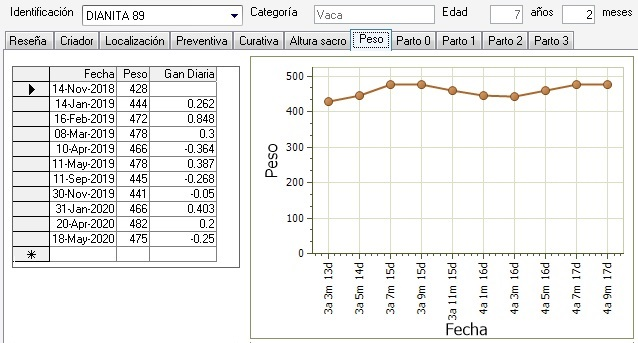
\includegraphics[scale=0.92]{img/ejpesos.jpg}
	 \end{center}
	 \caption{Ejemplo de seguimiento digital de peso en la res ``Dianita''. \label{ejpesos}}
\end{figure}

Los datos almacenados en este software, muestran registros de peso bimensual o trimestral, genealogía, suministro de medicamentos y producciones lecheras semanales.
No obstante, aún cuando este software ofrece una gran ventaja para el seguimiento de los datos, se encuentra limitado a las pocas licencias ofrecidas para su manejo. Por lo tanto es plausible considerar alternativas para el análisis, seguimiento de datos y toma de decisiones futuras, lo que justifica nuevamente la realización de este proyecto.

\chapter{CRISP - DM: ETAPA \#3 \\ Preparación de los datos} 
\label{crisp3}

En esta etapa, se procede a recolectar todos los datos análogos y digitales con los que cuenta en CA-SENA-POP, para almacenarlos de manera digital y proceder a analizar los datos mediante algoritmos en Matlab y/o Python. Es importante recalcar que para ambos software se requiere una estructura de datos en tablas debidamente organizadas, ya sea para tratarlos como $dataframes$, matrices, arreglos, o como tablas de archivos $^{*}.csv$.

\section{Recolección de datos} \label{datarecol}

Tal y como se mencionó en el capítulo anterior, los datos referentes a Peso, Leche y Alimentación, de cada una de las reses del CA-SENA-POP se encuentran registradas de manera física o digital; ya sea en hojas impresas como el ejemplar de la figura \ref{regleche1png}, así como también en bases de datos digitales como el de la figura \ref{tauruspng}. No obstante, estos datos \textbf{no} pueden ser importados directamente a algún software de procesamiento de datos. Esto puesto que para los datos físicos, se tienen algunas barreras y/o inconvenientes externos tales como los diferentes tipos de letra,  el estado físico de las paginas, y la diferencia entre los números de un ente registrado u otro; mientras que para los datos digitales, estos se encuentran almacenados en el software de pago de manera privada, siendo datos protegidos de acuerdo a la ley de ``Habeas data'', por lo que no pueden ser exportados directamente para manipulación del público.\\ % Feb  2023

% \subsection{Registros de ``Leche''}
Teniendo en cuenta que los datos de producción lechera se registran de manera manual, esta tarea es llevada a cabo por distintas personas. Desde aprendices hasta instructores y supervisores; por lo tanto, los datos son escritos por distintas personas, que manejan distintos tipos de letra, distinto orden, distintas practicas adecuadas de escritura, entre otras. Esto implica que los números registrados en las paginas físicas varíen de un tipo de letra a otra y deban ser analizados o copiados rigurosamente de manera digital. Además, es importante mencionar, que estas carpetas físicas de registro de datos, son expuestas a la intemperie, por lo que algunos registros han sido vulnerables ante lluvias, o sustancias que alteran el estado de la hoja de papel, dificultando así su interpretación a primera vista.\\

Es importante hacer esta observación, dado que por estas mismas circunstancias, \textbf{no} es posible extraer los datos de las tablas mediante algoritmos de inteligencia artificial de procesamiento de imágenes de manera consistente, pues estos datos pueden ser fácilmente tergiversados o malinterpretados como los ejemplares de la figura \ref{datosamanopng}.

\begin{figure}[H]
	 \begin{center}
	 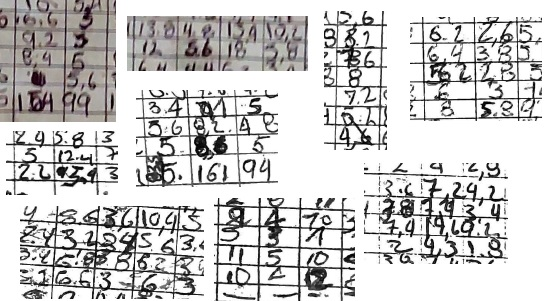
\includegraphics[scale=1.05]{img/datosamano.jpg}
	 \end{center}
	 \caption{Ejemplares de datos físicos con malas prácticas de escritura. \label{datosamanopng}}
\end{figure}

En cuanto a los registros de peso, dado que la cantidad de datos no es tan abrumadora a comparación de los registros de leche, estos datos son transcritos a archivos de excel y posteriormente a archivos con extensión $^{*}.csv$.

\section{Digitalización de los datos de producción lechera}

Teniendo en cuenta la descripción anterior, los datos fueron escaneados y posteriormente fueron transcritos de manera individual. Los datos utilizados en este trabajo consisten en los registros de producción lechera de distintas vacas que han entrado y salido de la producción ganadera, ya sea por motivos de compraventa, ingreso a gestación, salida por periodo de secado,  enfermedad, deceso, edad o cantidad de partos.\\

Los datos aquí utilizados comprenden fechas desde el 31 de Diciembre de 2018, hasta el 24 de Julio de 2022. En total se transcribieron de forma manual un total de $85.932$  datos, de los cuales, $37.956$ son datos numéricos representativos que pueden usarse para procesamiento de datos. Los $47.976$ datos restantes son datos categóricos que representan periodos de secado, horra, datos inexistentes o ilegibles, o registros desconocidos clasificados como datos NAN. Se cuenta con un total de 4 archivos pdf, en donde se almacenan los escaneos de los datos que comprenden esas fechas ya mencionadas.\\

Esta tarea de transcripción de datos tomó un tiempo aproximado de 1 semana;7 días, en jornadas de 8 horas cada día. Los datos que poseían dificultades de lectura e interpretación fueron corroborados con base en los datos de producción diaria neta y producción neta individual de cada vaca, datos existentes en las tablas escaneadas; por lo que se reduce el riesgo de transcripción de datos erróneos por causas humanas.

Aún sí existiese algún dato atípico o dato erróneo, esto puede corroborarse con la estructuración de los datos que se empleó para su análisis y que se explica en la sección a continuación.

\section{Reestructuración de los datos de leche}\label{reestructleche}
% \section{Datos de leche}
Una vez que se transcribieron los datos de manera individual para cada vaca. se procede a agrupar los datos en un archivo de excel organizado de la siguiente forma:

\subsection{Reestructuración inicial}

\begin{figure}[H]
	 \begin{center}
	 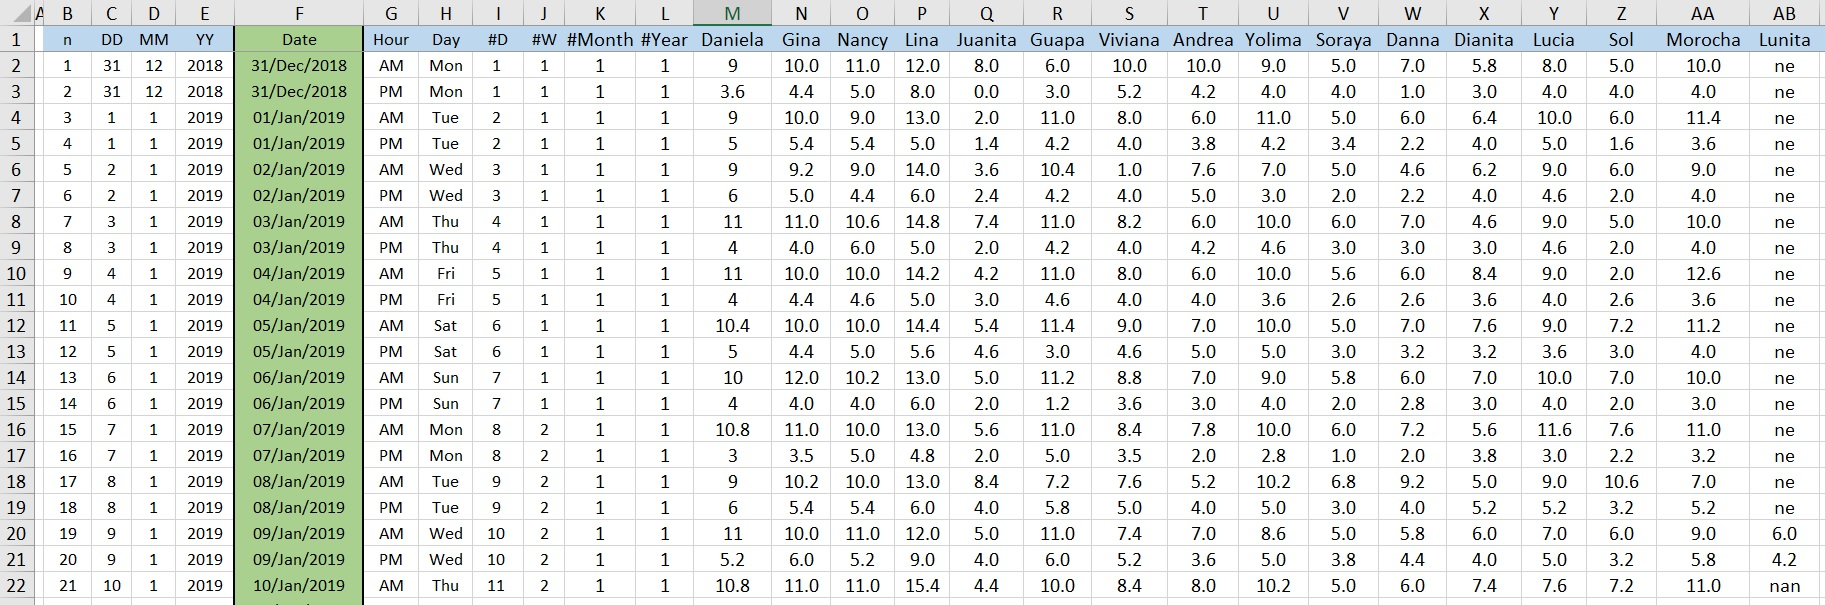
\includegraphics[scale=0.335]{img/dfinicial.jpg}
	 \end{center}
	 \caption{Reestructuración inicial de los datos de producción de leche transcritos. \label{dfinicialpng}}
\end{figure}

\begin{itemize}
    \item Cada fila, representa una \textbf{muestra - n} tomada en una \textbf{fecha (``DD/MM/AAAA'')} en una \textbf{franja horaria (AM o PM)}, en un \textbf{día de la semana (DAY y \#D)}, en una \textbf{semana (\#W)} , en un \textbf{mes (\#Month)} y en un \textbf{año (\#Year)} específico.
    \item Cada columna, representa una \textbf{vaca} que produjo una \textbf{cantidad de leche (valor numérico positivo)}.
    \item Cada 2 filas se tiene un cambio de fecha, pues se registran los datos de la mañana (AM) y también se registran los datos de la tarde (PM) como muestras separadas; más no como días distintos. Por lo tanto se tienen 2 muestras por cada día.
    \item En caso que una vaca no se encontrase en los registros de producción de leche para una fecha especifica y sus días anteriores, se cataloga como \textbf{vaca no existente} o \textbf{ne}
    \item En caso que una vaca muriera, los datos subsiguientes a esa fecha serán datos de tipo texto representados con la letra \textbf{M}.
    \item En caso que una vaca se vendiera,  los datos subsiguientes a esa fecha serán datos de tipo texto representados con la letra \textbf{V}.
    \item En caso que una vaca se encontrase en periodo de Horra,  los datos subsiguientes a esa fecha serán datos de tipo texto representados con la letra \textbf{H}, hasta indicado lo contrario.
    \item En caso que una vaca no se encontrase en periodo determinado, fuera por falta de preñes, horra, u otro motivo desconocido,  los datos subsiguientes a esa fecha aproximada serán datos de tipo texto representados con las letras \textbf{UL}, haciendo referencia a ``Unknown-Location''.
    \item En caso que una vaca se encontrase en periodo de secado, los datos subsiguientes a esa fecha serán datos de tipo texto representados con la letra \textbf{S}, hasta que se reincorpore tras el periodo de secado o hasta que se avise lo contrario (Muerte, Venta, Horra).
    \item En caso que un registro de producción de leche no haya sido transcrito, ya sea por malas practicas de escritura del documento físico, datos ilegibles o datos inexistentes, la casilla tendrá un valor de texto representado con las letras \textbf{NAN}, \textbf{haciendo referencia a un dato desconocido o dato inexistente por motivo desconocido}.
    \item En caso de tener valores numéricos 0, este valor es dejado como 0, si se muestra reincidencia en los días subsiguientes (suele suceder en fechas cercanas al periodo de secado), este valor será dejado así pues desde la práctica de toma de datos se ha considerado como una extracción de una cantidad de leche aproximadamente nula. No obstante, ya se ha mencionado que el dominio de los valores númericos de producciones de leche son \textbf{enteros positivos}.
    \item De las observaciones anteriores es importante agregar que los datos numéricos no pueden ser negativos.
    \item Se tiene un total de 2604 muestras para cada vaca, ya sea numérico o categórico. Se hace así pues las columnas de la matriz deben tener la misma cantidad de datos
    \item Se obtuvieron muestras de un total de 33 vacas distintas.
    \item Se maneja el dato desconocido con la denominación NAN y no con otro símbolo como el signo de interrogación ``?'', por motivos de formato al momento de transcribir los datos a Microsoft Excel.
\end{itemize}

\subsection{``Debugging'' y verificación de datos}

Como la transcripción de los datos se realiza de forma manual, existe el riesgo de añadir error humano a mediciones que ya cuentan con errores de medición y escritura. Para disminuir este error de transcripción, se verificó uno a uno los valores, antes, durante y después del proceso de transcripción. No obstante puede que se hayan pasado valores por alto como reflejo de un error humano.\\

Para ello, una vez obtenida la matriz agrupada en Excel, se verifican los tipos de datos y se corrobora que la cantidad neta de cada grupo sumen la cantidad total de datos. En caso contrario, el valor en cuestión se puede identificar el índice de la(s) muestra(s) no identificada(s) y mediante la fecha en la que fue(ron)  tomada(s), se puede corroborar tanto en la tabla de Excel, como en los archivos pdf escaneados. 

\subsection{Reestructuración numérica}

Notese que en la reestructuración inicial se puede observar que los datos pueden ser numéricos o categóricos, no obstante esto dificulta su análisis matricial en el software de Matlab por lo que se procede a tener algunas consideraciones adicionales.

\begin{itemize}
    \item En caso de muerte o venta, se considera como dato de valor numérico 0.0, pues se considera como una producción de leche nula dado que no se puede extraer leche de un animal muerto o vendido, mas no obstante, no es considerado como valor de tipo NAN, \textbf{pues se considera NAN un valor que no pudo ser medido y se desconoce el motivo.}
    \item Como los datos no pueden ser biológica ni físicamente negativos; en caso que una vaca no existiese en fechas anteriores a la fecha de registro (los datos \textbf{ne}), se cambiará el valor categórico \textbf{ne} por un \textbf{-1}.
\end{itemize}


Así pues, se conforma un primer archivo de excel con todos los registros existentes hasta la fecha del 24 de Julio del 2022. Es importante mencionar que el balance existente entre datos numéricos útiles para procesamiento y análisis, con datos de tipo NAN es  aproximadamente de 90\% contra menos del 10\% respectivamente. Y en comparación de datos de tipo NAN con datos conocidos, ya sean numéricos representativos o datos categóricos transformados; el porcentaje de balance disminuye hasta un 5.6\%.\\

De esta manera se puede considerar que los datos de tipo NAN no son significativos para los análisis posteriores, y pueden pasarse por alto o reemplazarse con métodos de imputación, sin afectar negativamente los análisis a futuro.
% se puede corroborar en DATAF SENA 2022 AGO 21 DATA RAW NUM - SUPER VACA

\pagebreak

\subsection{Clasificación, Selección y Agrupación de datos de leche}
Teniendo en cuenta la base de datos estructurada en el punto anterior, es importante cuestionarse sí estos datos pueden representar matemáticamente toda la producción de leche del CA-SENA-POP, pues aunque son datos que evidencian la producción neta de la granja, estos datos dispersos no permiten una aproximación mediante funciones y/o modelos matemáticos, ni mucho menos posibilitan el modelamiento dinámico mediante ecuaciones diferenciales. Por lo tanto es imprescindible estimar una o varias funciones que representen de manera aproximada, los datos obtenidos.\\

Es decir, que se debe considerar un ajuste de curvas a los datos existentes para aproximar la producción neta mediante funciones y modelos matemáticos. Por otra parte es importante tener en cuenta que las producciones de leche de cada animal, varían según el número de partos que hayan experimentado con anterioridad. Las vacas primíparas que recién están produciendo leche, no tendrán un rendimiento equiparable a comparación de las vacas que ya se encuentran en un 3er o 4to parto; en consecuencia es plausible realizar una clasificación de vacas por su cantidad de partos y observar el comportamiento de las producciones lecheras para cada grupo de partos.\\

\subsubsection{Clasificación de Datos}

Así pues, con base en las observaciones anteriores y partiendo de los datos existentes del CA-SENA-POP, tendremos 6 grupos distintos de partos. $Parto_{i}$, con i=1...6\\

Notese que los datos previamente estructurados cuentan con los registros de producción lechera desde el año 2018 hasta el año 2022, con todos los registros existentes para cada una de las vacas. No obstante, en este periodo de tiempo, en los documentos físicos no se específica el número de parto de cada animal. En algunos casos se ha hecho la observación, mas sin embargo no aplica para todas las reses. Observese además, que los partos entre las vacas no están sincronizados; por lo que esta clasificación permite identificar qué vacas son contemporáneas con otras. Por ende, es necesario acudir a la base de datos digital del software TaurusWebs con el que cuenta el centro agropecuario; para hacer una validación cruzada de los datos.\\

Una vez obtenido el permiso y una copia de la base de datos actual, suministrada por el encargado Daniel Cobo. se puede acceder al software con una versión gratuita de prueba; licencia que satisface la posibilidad de consultar las fechas de parto de cada bovino. Esto se logra gracias a la trazabilidad con la que cuenta este software y se puede hacer contraste con los datos previamente estructurados; dándose la posibilidad de clasificar los datos según el parto al que corresponden para cada ternera:

\begin{figure}[H]
	 \begin{center}
	 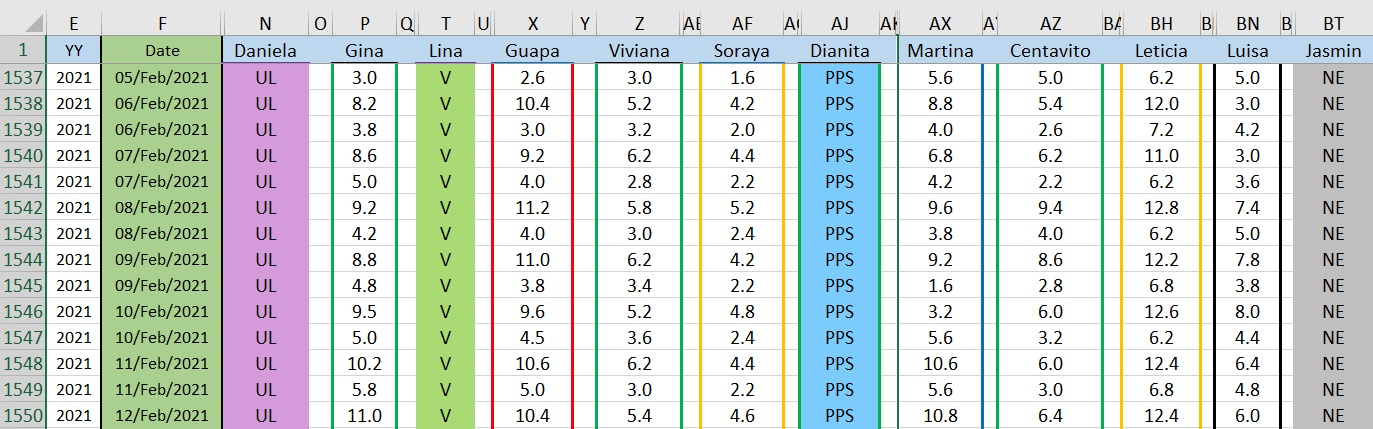
\includegraphics[scale=0.45]{img/dfcolorpartos.jpg}
	 \end{center}
	 \caption{Clasificación de datos por \#Parto para cada vaca. \label{colorpartospng}}
\end{figure}

En la figura anterior se puede observar que la clasificación de los partos se realiza con base en la estructuración de datos tanto categóricos como numéricos. Esto con el objetivo de diferenciar de manera visual entre un periodo de producción de leche a un periodo de secado (Casilla blanca con borde de color y casillas coloreadas de color azul respectivamente). No obstante una vez realizada la clasificación, selección y agrupación de datos; las matrices usadas en los análisis posteriores con algoritmos en Matlab, manejan la estructuración numérica descrita en la sub-sección anterior.\\

Percatese que al tener 6 grupos de partos en el CA-SENA-POP, se utiliza un código de colores para la clasificación de producción por \# de Parto, siendo esta la siguiente:

% Please add the following required packages to your document preamble:
% \usepackage{graphicx}
% \usepackage[table,xcdraw]{xcolor}
% If you use beamer only pass "xcolor=table" option, i.e. \documentclass[xcolor=table]{beamer}
\begin{table}[H]
\centering
\caption{Código de colores por número de parto}
\label{colorpartos}
\resizebox{\textwidth}{!}{%
\begin{tabular}{|
>{\columncolor[HTML]{FFCE93}}c |
>{\columncolor[HTML]{000000}}c |
>{\columncolor[HTML]{1122C6}}c |
>{\columncolor[HTML]{32CB00}}c |
>{\columncolor[HTML]{FFFE65}}c |
>{\columncolor[HTML]{EF3B3B}}c |
>{\columncolor[HTML]{AD71EB}}c |}
\hline
\textit{\textbf{\begin{tabular}[c]{@{}c@{}}Color del\\  borde\end{tabular}}} &
  {\color[HTML]{FFFFFF} \textit{\textbf{Negro}}} &
  {\color[HTML]{FFFFFF} \textit{\textbf{Azul}}} &
  \textit{\textbf{Verde}} &
  \textit{\textbf{Amarillo}} &
  \textit{\textbf{Rojo}} &
  \textit{\textbf{Morado}} \\ \hline
\textit{\textbf{\begin{tabular}[c]{@{}c@{}}\# de \\ Parto\end{tabular}}} &
  \cellcolor[HTML]{C0C0C0}\textit{\textbf{1}} &
  \cellcolor[HTML]{A3E1F3}\textit{\textbf{2}} &
  \cellcolor[HTML]{A1DA8E}\textit{\textbf{3}} &
  \cellcolor[HTML]{FFFFC7}\textit{\textbf{4}} &
  \cellcolor[HTML]{F39E9E}\textit{\textbf{5}} &
  \cellcolor[HTML]{B791DE}\textit{\textbf{6}} \\ \hline
\end{tabular}%
}
\end{table}

Así pues, se obtienen 6 grupos de un tamaño variable de vacas para cada número de parto. Esta clasificación se puede observar en la tabla \ref{porpartos}. % la tabla gigante de colores que no se deja poner label

\subsubsection{Selección de Datos}

Una de las primeras observaciones obtenidas al realizar la agrupación por partos; es que los datos existentes que han sido agrupados no poseen igual cantidad de datos para cada res. Esto se produce dado que los partos varían en cuestión de duración para cada animal. En primera instancia esto no debería suponer un problema significativo, pues en caso que los partos posean una ligera variabilidad de muestras; bastaría con ``rellenar'' los datos faltantes con ceros o con imputación de datos como la media o la moda; ó por otra parte, bastaría con realizar una agrupación con igual cantidad de muestras.\\

Sin embargo, esta contra medida no puede ser llevada a cabo en razón de que los datos existentes facilitan la agrupación por partos, mas no garantiza que los datos de un parto en específico se encuentren disponibles en su totalidad. En otras palabras, muchos de los datos que se tienen para cada parto son datos de inicio de producción o finalización de producción de leche de las terneras, tanto para las que fallecen, para las que se venden, así como también, para las que a fecha del 31 de Diciembre del 2018 ya se encontraban en periodo productivo.\\

Si se realiza una representación visual individual de los datos, se puede observar claramente que algunas reses tienen muy pocos datos, lo que ``recargaría'' la distribución hacia los extremos, dificultando su análisis descriptivo. Por otra parte, si se hace un contraste de datos teniendo como punto de referencia el inicio de la producción o su finalización en el periodo de secado, la tabla de registros permite evidenciar el desbalance que manifiestan los datos:

\begin{figure}[H]
	 \begin{center}
	 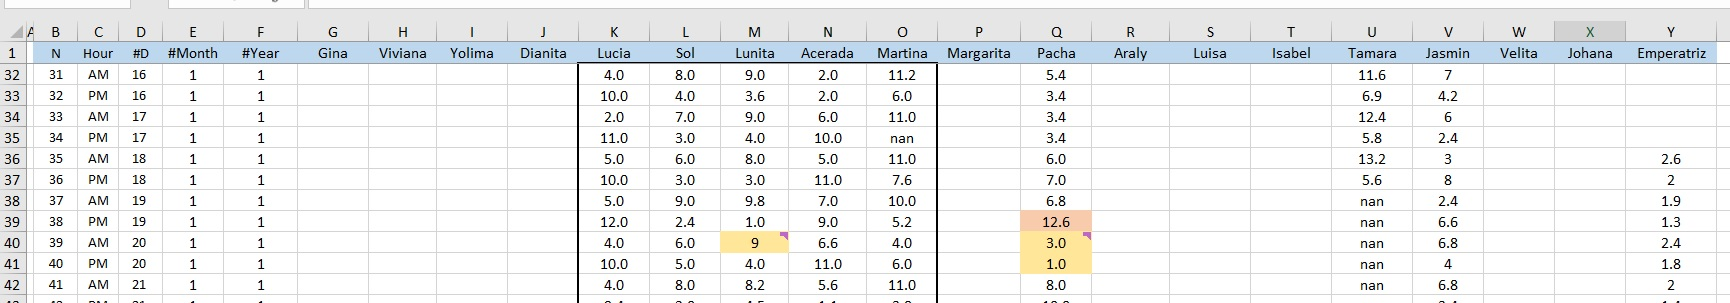
\includegraphics[scale=0.34]{img/partosincompletos.jpg}
	 \end{center}
	 \caption{Desbalance de datos en agrupación inicial por partos. \label{partosincompletospng}}
\end{figure}

En la figura anterior, se evidencia claramente el desbalance mencionado. Si se observan mas a fondo los datos presentes en el archivo de Excel; 13 de las 19 reses cuentan con menos de la mitad de muestras de producción lechera tras haber parido por primera vez. Solo una de ellas, manifiesta un exceso de registros antes de entrar en periodo de secado; y 5 mamíferos restantes aparentan tener la cantidad de muestras suficientes para representar el grupo de vacas primíparas. Las 5 vacas en cuestión son ``Lucia'', ``Sol'', ``Lunita'', ``Acerada'' y ``Martina''.\\

Finalmente, aunque todas las reses cuentan con la misma cantidad de datos, se procede a seleccionar únicamente a 3 de ellas que coinciden en el inicio y finalización de la producción de leche (``Sol'', ``Lunita'', ``Acerada''). Mientras que las otras 2; a pesar de tener la misma cantidad de muestras, presentan desfases en el inicio y finalización de la etapa productiva (Lucia y Martina). De esta forma, se puede generar la primera representación visual de los datos mediante un gráfico de dispersión, tal y como se observa en la  figura \ref{scatterparto1png}.

\begin{figure}[H]
	 \begin{center}
	 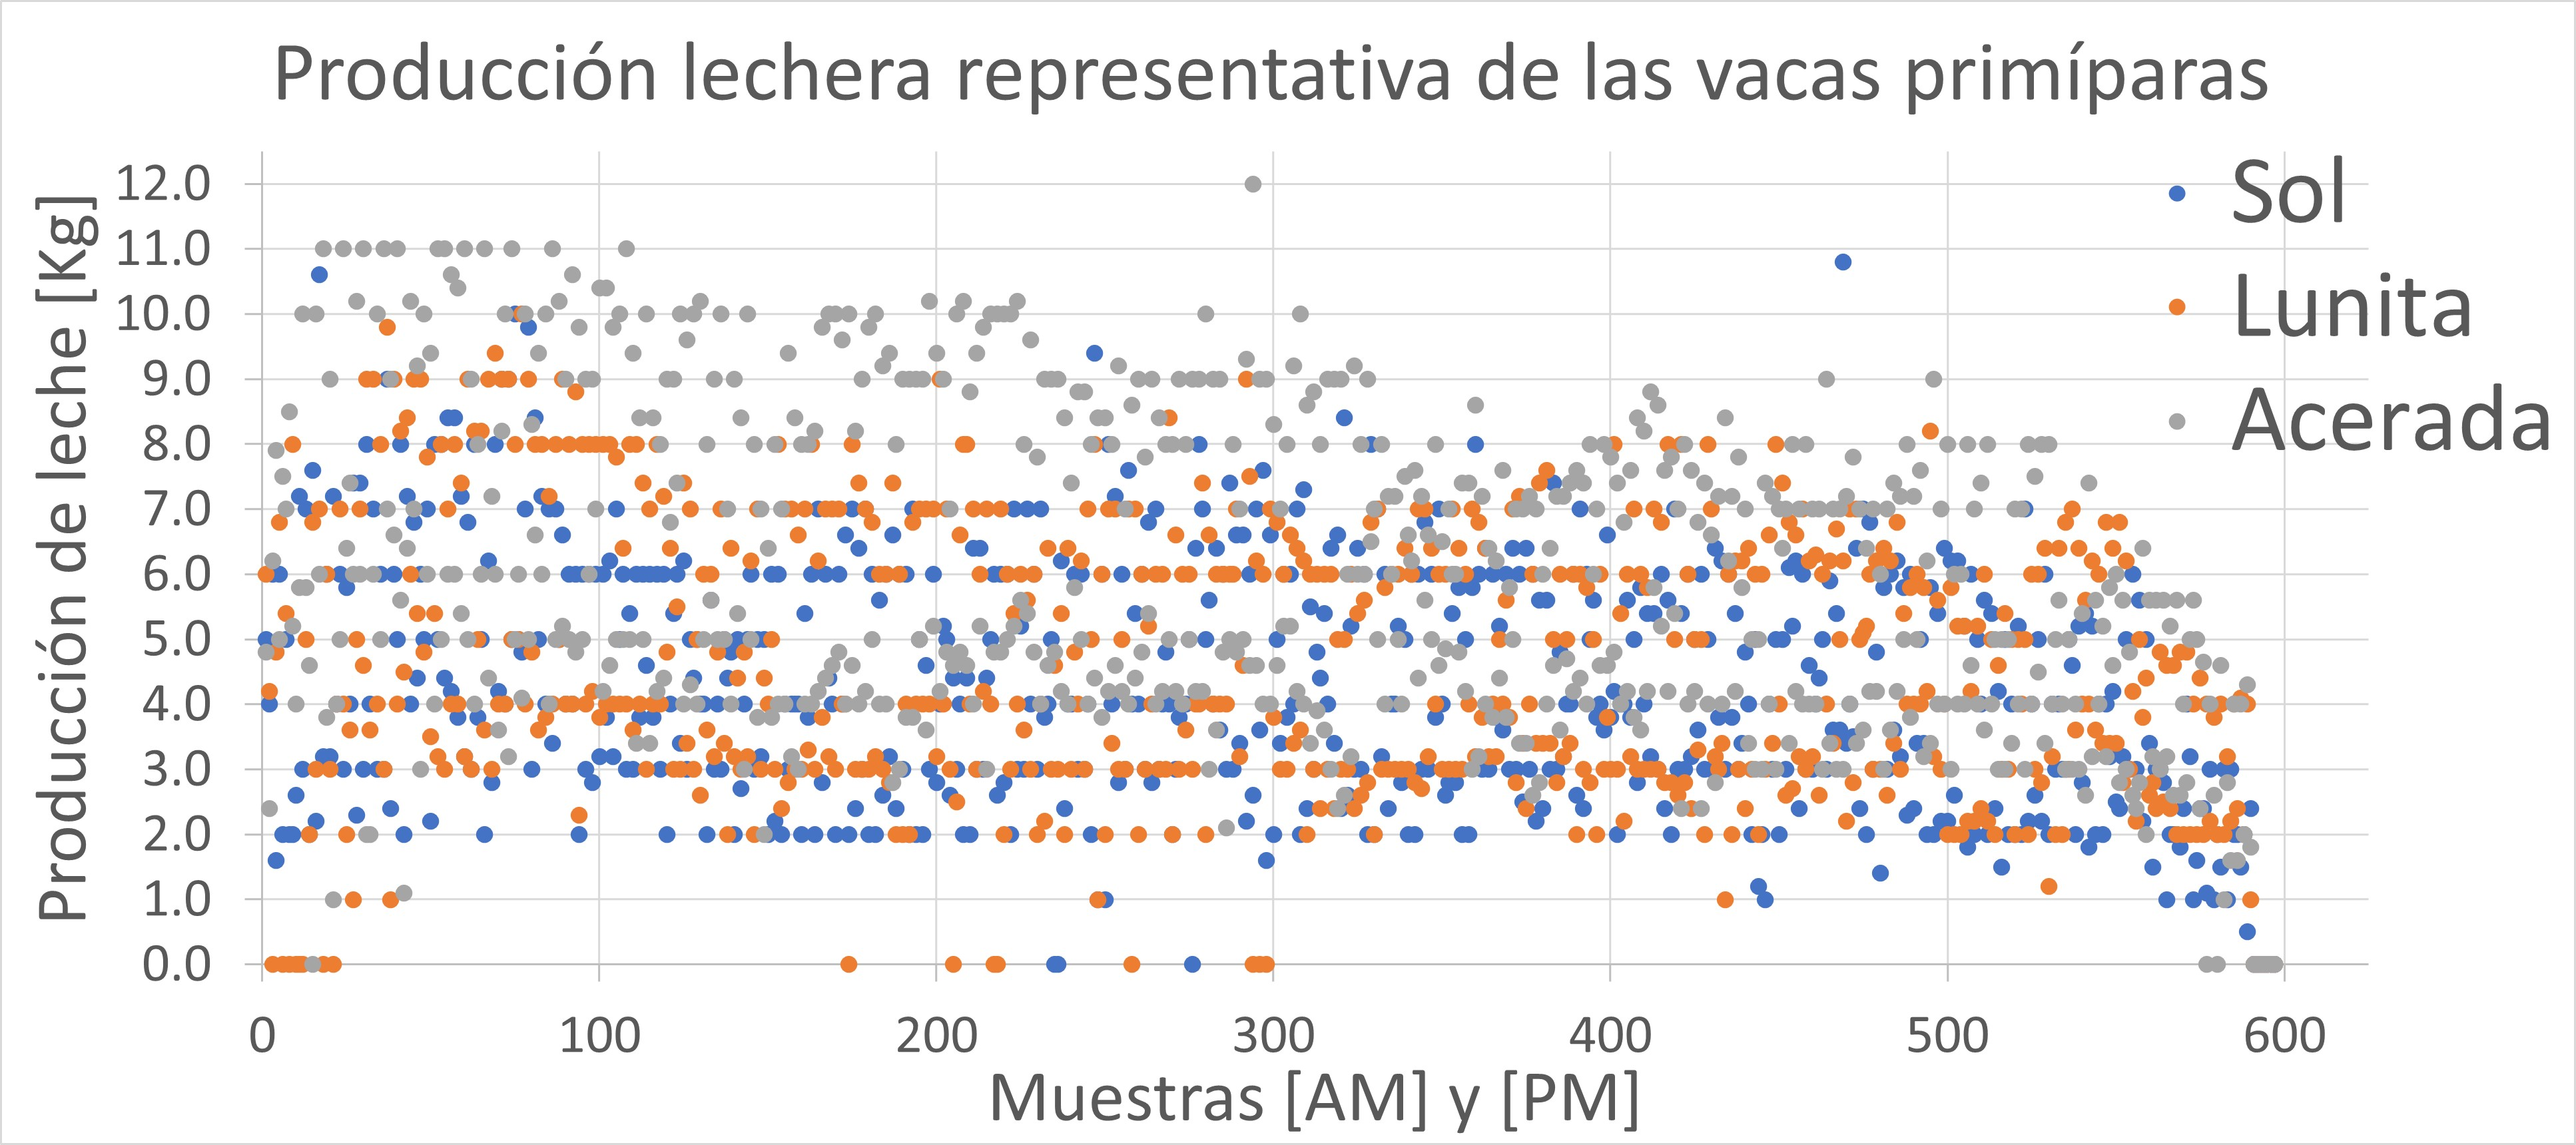
\includegraphics[scale=0.452]{img/scatterparto1.jpg}
	 \end{center}
	 \caption{Gráfico de dispersión para representar la producción lechera de las vacas primíparas. \label{scatterparto1png}}
\end{figure}

\subsubsection{Agrupación de Datos}

El resultado obtenido tras realizar la primer representación visual de datos da un idea de cómo no se deben utilizar los datos para los análisis matemáticos. Pues se observa que al tener muestras matutinas y vespertinas juntas, no se logran diferenciar los datos correspondientes a cada intervalo. Además, el intervalo de tiempo es de 305 días aproximadamente y al manejar ambos tipos de muestras, se tiene un total de 610 datos en el eje horizontal. Por ende, como medida inicial, se opta por realizar un análisis independiente para las muestras obtenidas en diferentes horas del día, procediendo con una representación individual como se observa a continuación:

\begin{figure}[H]
	 \begin{center}
	 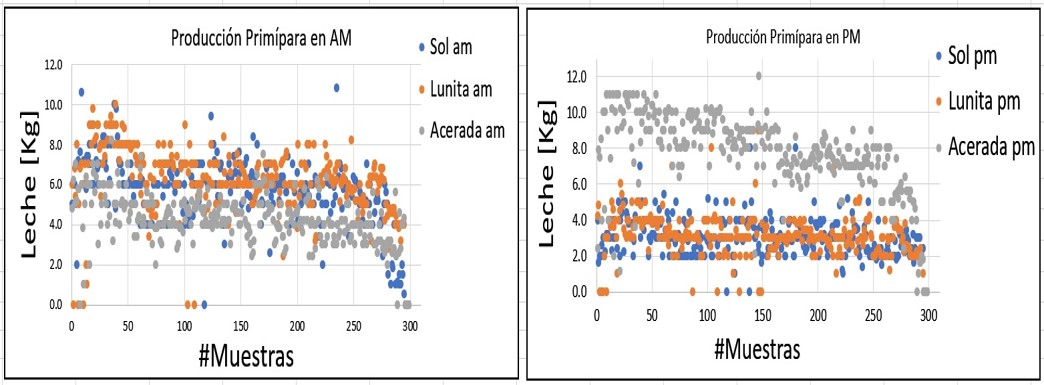
\includegraphics[scale=0.575]{img/desfaseAMPM.jpg}
	 \end{center}
	 \caption{Gráfico de dispersión para Muestras matutinas y vespertinas. \label{desfaseAMPMpng}}
\end{figure}

En primera instancia parece que la gráfica anterior no presenta ningún inconveniente, a pesar de ello, se puede notar un leve desajuste entre los valores vespertinos; pues los valores de la res denominada como ``Acerada'', muestran una lejanía con los otros datos en el horario de la tarde. Esto genera ciertas inquietudes teniendo en cuenta que las muestras matutinas tienden a ser mayores que las muestras vespertinas para la mayoría de las reses de este estudio. En virtud de que el lapso que existe entre una muestra matutina con una vespertina en un mismo día es de aproximadamente 10 horas; mientras que el lapso entre una muestra vespertina y una muestra matutina es de aproximadamente 14 horas; no sería de extrañar que al tener mayor tiempo de recuperación, se le pueda extraer mayor cantidad de leche a la vaca.

Lo anterior se presta para realizar nuevamente una corroboración de los datos con los datos manuales existentes y la tabla de datos de la estructuración inicial; con lo que se observa que al realizar la ``alineación'' de datos tras la agrupación por partos; los datos matutinos de la res en cuestión han quedado ``alineados'' con los datos vespertinos de las otras reses. Esto quiere decir que la figura \ref{desfaseAMPMpng} debe cambiarse por la figura \ref{AMPMsindesfasepng}:


\begin{figure}[H]
	 \begin{center}
	 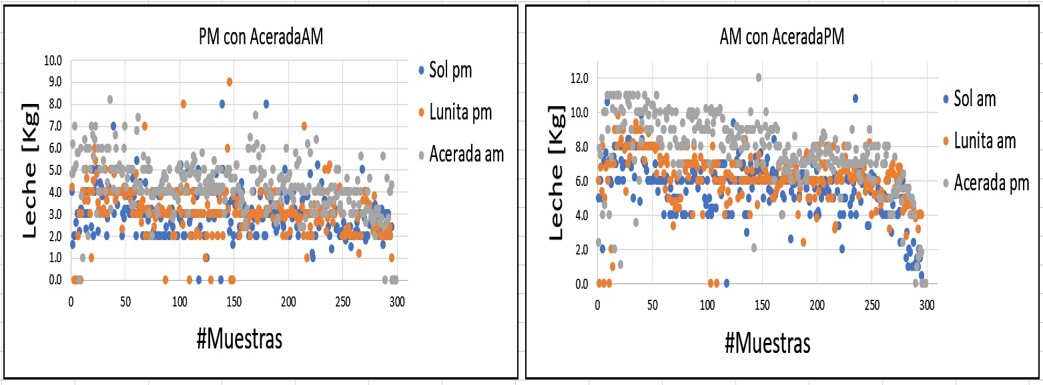
\includegraphics[scale=0.5835]{img/AMPMsindesfase.jpg}
	 \end{center}
	 \caption{Gráfico de dispersión para Muestras matutinas y vespertinas. \label{AMPMsindesfasepng}}
\end{figure}


De acuerdo con la situación anterior, se concluye que realizar un análisis por franja horaria puede llevar a errores futuros o a reincidentes corroboraciones de datos, siendo esto último una tarea agobiante para el caso de estudio; por lo que se decide considerar únicamente análisis con la producción neta diaria de cada animal. De esta forma se repite el proceso para los otros grupos de partos obteniéndose los gráficos de dispersión de la figura \ref{svnetaspng} y obteniéndose un conjunto total de 28 reses para análisis futuros; que se puede observar en la tabla \ref{porpartosfin}.

% Please add the following required packages to your document preamble:
% \usepackage{multirow}
% \usepackage{graphicx}
% \usepackage[table,xcdraw]{xcolor}
% If you use beamer only pass "xcolor=table" option, i.e. \documentclass[xcolor=table]{beamer}
%=======================================================
% Please add the following required packages to your document preamble:
% \usepackage{multirow}
% \usepackage{graphicx}
% \usepackage[table,xcdraw]{xcolor}
% If you use beamer only pass "xcolor=table" option, i.e. \documentclass[xcolor=table]{beamer}
% Please add the following required packages to your document preamble:
% \usepackage{multirow}
% \usepackage{graphicx}
% \usepackage[table,xcdraw]{xcolor}
% If you use beamer only pass "xcolor=table" option, i.e. \documentclass[xcolor=table]{beamer}
\begin{table}[H]
\centering
\caption{Agrupación final de vacas por \# de partos}
\label{porpartosfin}
\resizebox{\textwidth}{!}{%
\begin{tabular}{|
>{\columncolor[HTML]{FFCE93}}c |
>{\columncolor[HTML]{C0C0C0}}c |
>{\columncolor[HTML]{A3E1F3}}c 
>{\columncolor[HTML]{A3E1F3}}c |
>{\columncolor[HTML]{A1DA8E}}c 
>{\columncolor[HTML]{A1DA8E}}c |
>{\columncolor[HTML]{FFFFC7}}c 
>{\columncolor[HTML]{FFFFC7}}c |
>{\columncolor[HTML]{F39E9E}}c |
>{\columncolor[HTML]{B791DE}}c |}
\hline
\textit{\textbf{\# de Parto}} &
  \cellcolor[HTML]{000000}{\color[HTML]{FFFFFF} \textit{\textbf{1}}} &
  \multicolumn{2}{c|}{\cellcolor[HTML]{1122C6}{\color[HTML]{FFFFFF} \textit{\textbf{2}}}} &
  \multicolumn{2}{c|}{\cellcolor[HTML]{32CB00}\textit{\textbf{3}}} &
  \multicolumn{2}{c|}{\cellcolor[HTML]{FFFE65}\textit{\textbf{4}}} &
  \cellcolor[HTML]{EF3B3B}\textit{\textbf{5}} &
  \cellcolor[HTML]{AD71EB}\textit{\textbf{6}} \\ \hline
\cellcolor[HTML]{FFCE93} &
  \textit{\textbf{Acerada}} &
  \multicolumn{1}{c|}{\cellcolor[HTML]{A3E1F3}\textit{\textbf{Dianita}}} &
  \textit{\textbf{Pacha}} &
  \multicolumn{1}{c|}{\cellcolor[HTML]{A1DA8E}\textit{\textbf{Fernanda}}} &
  \textit{\textbf{Martina}} &
  \multicolumn{1}{c|}{\cellcolor[HTML]{FFFFC7}\textit{\textbf{Centavito}}} &
  \textit{\textbf{Muchira}} &
  \textit{\textbf{Andrea}} &
  \textit{\textbf{Andrea}} \\ \cline{2-10} 
\cellcolor[HTML]{FFCE93} &
  \textit{\textbf{Lunita}} &
  \multicolumn{1}{c|}{\cellcolor[HTML]{A3E1F3}\textit{\textbf{Gina}}} &
  \textit{\textbf{Sol}} &
  \multicolumn{1}{c|}{\cellcolor[HTML]{A1DA8E}\textit{\textbf{Guapa}}} &
  \textit{\textbf{Morocha}} &
  \multicolumn{1}{c|}{\cellcolor[HTML]{FFFFC7}\textit{\textbf{Dianita}}} &
  \textit{\textbf{Soraya}} &
  \textit{\textbf{Guapa}} &
  \textit{\textbf{Guapa}} \\ \cline{2-10} 
\cellcolor[HTML]{FFCE93} &
  \textit{\textbf{Sol}} &
  \multicolumn{1}{c|}{\cellcolor[HTML]{A3E1F3}\textit{\textbf{Juanita}}} &
  \textit{\textbf{Viviana}} &
  \multicolumn{1}{c|}{\cellcolor[HTML]{A1DA8E}\textit{\textbf{Juanita}}} &
  \textit{\textbf{Sol}} &
  \multicolumn{1}{c|}{\cellcolor[HTML]{FFFFC7}\textit{\textbf{Leticia}}} &
  \textit{\textbf{Viviana}} &
  \textit{\textbf{}} &
  \textit{\textbf{}} \\ \cline{2-10} 
\multirow{-4}{*}{\cellcolor[HTML]{FFCE93}\textit{\textbf{\begin{tabular}[c]{@{}c@{}}Vacas \\ participantes\end{tabular}}}} &
  \textit{\textbf{}} &
  \multicolumn{1}{c|}{\cellcolor[HTML]{A3E1F3}\textit{\textbf{Lucia}}} &
  \textit{\textbf{}} &
  \multicolumn{1}{c|}{\cellcolor[HTML]{A1DA8E}\textit{\textbf{Leticia}}} &
  \textit{\textbf{}} &
  \multicolumn{1}{c|}{\cellcolor[HTML]{FFFFC7}\textit{\textbf{Morocha}}} &
  \textit{\textbf{}} &
  \textit{\textbf{}} &
  \textit{\textbf{}} \\ \hline
\end{tabular}%
}
\end{table}
%=======================================================
% Corregir que el parto 4 no salió bien la leyenda >:C

\begin{figure}[H]
	 \begin{center}
	 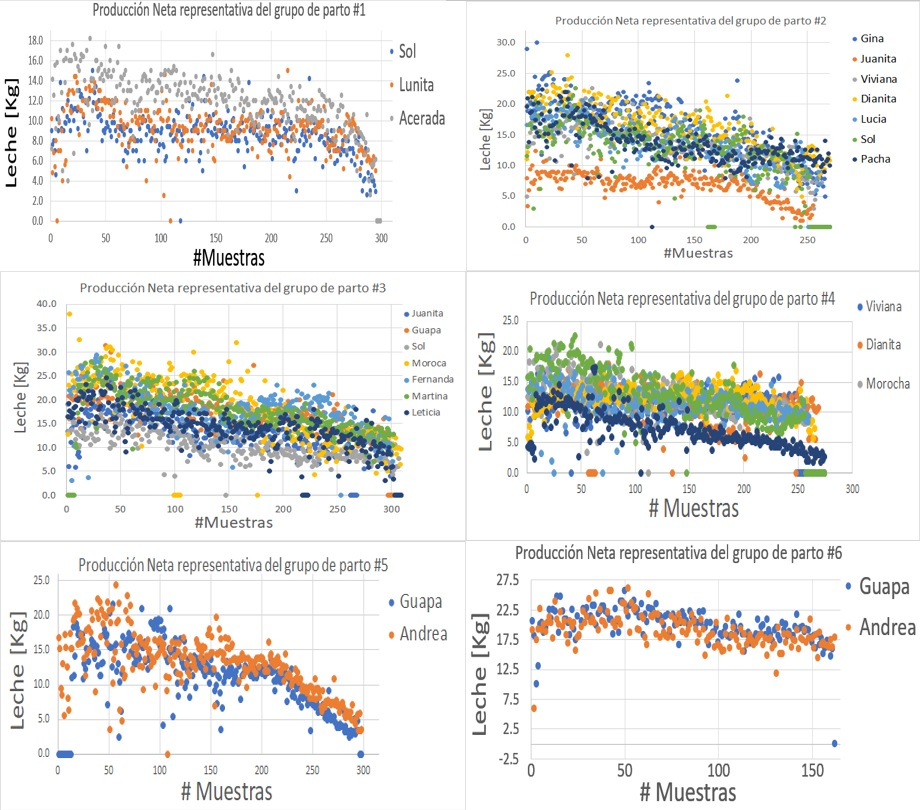
\includegraphics[scale=0.675]{img/svnetas.jpg}
	 \end{center}
	 \caption{Gráfico de dispersión para cada grupo de partos. \label{svnetaspng}}
\end{figure}


% , dando paso en este análisis, que la agrupación de datos de dispersión por partos se le denomine como datos de dispersión neta de ``supervaca'' del parto 1:

% \begin{figure}[H]
% 	 \begin{center}
% 	 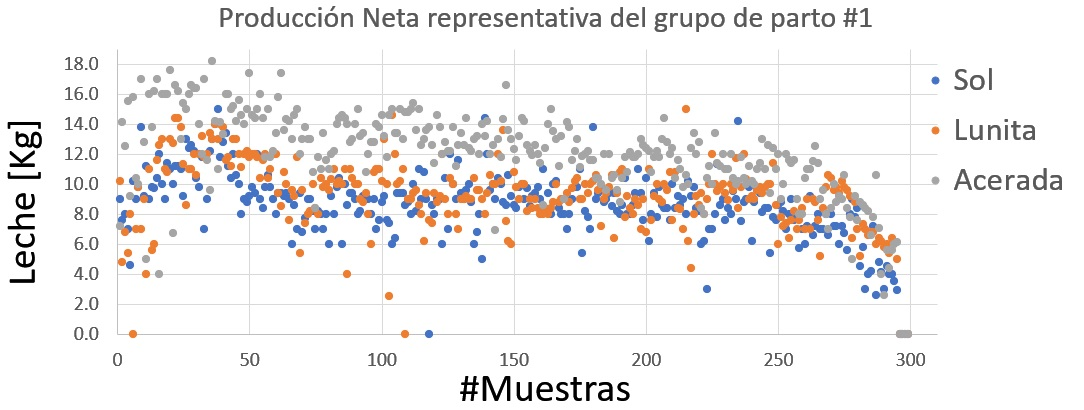
\includegraphics[scale=0.6]{img/svnetap1.jpg}
% 	 \end{center}
% 	 \caption{Gráfico de dispersión para registros de producción neta en vacas primíparas . \label{desfaseAMPMpng}}
% \end{figure}

%================================================================================================
% Please add the following required packages to your document preamble:
% \usepackage{multirow}
% \usepackage{graphicx}
% \usepackage[table,xcdraw]{xcolor}
% If you use beamer only pass "xcolor=table" option, i.e. \documentclass[xcolor=table]{beamer}
% Please add the following required packages to your document preamble:
% \usepackage{multirow}
% \usepackage{graphicx}
% \usepackage[table,xcdraw]{xcolor}
% If you use beamer only pass "xcolor=table" option, i.e. \documentclass[xcolor=table]{beamer}
\begin{table}[H]
\centering
\caption{Agrupación de vacas por \# de partos}
\label{porpartos}
\resizebox{\textwidth}{!}{%
\begin{tabular}{|c|ccccc|}
\hline
\rowcolor[HTML]{FFCE93} 
\textit{\textbf{\begin{tabular}[c]{@{}c@{}}\# de \\ Parto\end{tabular}}} &
  \multicolumn{5}{c|}{\cellcolor[HTML]{FFCE93}\textit{\textbf{\begin{tabular}[c]{@{}c@{}}Vacas \\ participantes\end{tabular}}}} \\ \hline
\rowcolor[HTML]{C0C0C0} 
\cellcolor[HTML]{000000}{\color[HTML]{FFFFFF} } &
  \multicolumn{1}{c|}{\cellcolor[HTML]{C0C0C0}\textit{\textbf{Gina}}} &
  \multicolumn{1}{c|}{\cellcolor[HTML]{C0C0C0}\textit{\textbf{Viviana}}} &
  \multicolumn{1}{c|}{\cellcolor[HTML]{C0C0C0}\textit{\textbf{Yolima}}} &
  \multicolumn{1}{c|}{\cellcolor[HTML]{C0C0C0}\textit{\textbf{Dianita}}} &
  \textit{\textbf{Lucia}} \\ \cline{2-6} 
\rowcolor[HTML]{C0C0C0} 
\cellcolor[HTML]{000000}{\color[HTML]{FFFFFF} } &
  \multicolumn{1}{c|}{\cellcolor[HTML]{C0C0C0}\textit{\textbf{Pacha}}} &
  \multicolumn{1}{c|}{\cellcolor[HTML]{C0C0C0}\textit{\textbf{Araly}}} &
  \multicolumn{1}{c|}{\cellcolor[HTML]{C0C0C0}\textit{\textbf{Luisa}}} &
  \multicolumn{1}{c|}{\cellcolor[HTML]{C0C0C0}\textit{\textbf{Isabel}}} &
  \textit{\textbf{Tamara}} \\ \cline{2-6} 
\rowcolor[HTML]{C0C0C0} 
\cellcolor[HTML]{000000}{\color[HTML]{FFFFFF} } &
  \multicolumn{1}{c|}{\cellcolor[HTML]{C0C0C0}\textit{\textbf{Sol}}} &
  \multicolumn{1}{c|}{\cellcolor[HTML]{C0C0C0}\textit{\textbf{Lunita}}} &
  \multicolumn{1}{c|}{\cellcolor[HTML]{C0C0C0}\textit{\textbf{Acerada}}} &
  \multicolumn{1}{c|}{\cellcolor[HTML]{C0C0C0}\textit{\textbf{Martina}}} &
  \textit{\textbf{Margarita}} \\ \cline{2-6} 
\rowcolor[HTML]{C0C0C0} 
\multirow{-4}{*}{\cellcolor[HTML]{000000}{\color[HTML]{FFFFFF} \textit{\textbf{1}}}} &
  \multicolumn{1}{c|}{\cellcolor[HTML]{C0C0C0}\textit{\textbf{Jasmin}}} &
  \multicolumn{1}{c|}{\cellcolor[HTML]{C0C0C0}\textit{\textbf{Velita}}} &
  \multicolumn{1}{c|}{\cellcolor[HTML]{C0C0C0}\textit{\textbf{Johana}}} &
  \multicolumn{1}{c|}{\cellcolor[HTML]{C0C0C0}\textit{\textbf{Emperatriz}}} &
  \textit{\textbf{}} \\ \hline
\rowcolor[HTML]{A3E1F3} 
\cellcolor[HTML]{1122C6}{\color[HTML]{FFFFFF} } &
  \multicolumn{1}{c|}{\cellcolor[HTML]{A3E1F3}\textit{\textbf{Gina}}} &
  \multicolumn{1}{c|}{\cellcolor[HTML]{A3E1F3}\textit{\textbf{Juanita}}} &
  \multicolumn{1}{c|}{\cellcolor[HTML]{A3E1F3}\textit{\textbf{Guapa}}} &
  \multicolumn{1}{c|}{\cellcolor[HTML]{A3E1F3}\textit{\textbf{Viviana}}} &
  \textit{\textbf{}} \\ \cline{2-6} 
\rowcolor[HTML]{A3E1F3} 
\cellcolor[HTML]{1122C6}{\color[HTML]{FFFFFF} } &
  \multicolumn{1}{c|}{\cellcolor[HTML]{A3E1F3}\textit{\textbf{Fernanda}}} &
  \multicolumn{1}{c|}{\cellcolor[HTML]{A3E1F3}\textit{\textbf{Acerada}}} &
  \multicolumn{1}{c|}{\cellcolor[HTML]{A3E1F3}\textit{\textbf{Martina}}} &
  \multicolumn{1}{c|}{\cellcolor[HTML]{A3E1F3}\textit{\textbf{Centavito}}} &
  \textit{\textbf{}} \\ \cline{2-6} 
\rowcolor[HTML]{A3E1F3} 
\cellcolor[HTML]{1122C6}{\color[HTML]{FFFFFF} } &
  \multicolumn{1}{c|}{\cellcolor[HTML]{A3E1F3}\textit{\textbf{Andrea}}} &
  \multicolumn{1}{c|}{\cellcolor[HTML]{A3E1F3}\textit{\textbf{Yolima}}} &
  \multicolumn{1}{c|}{\cellcolor[HTML]{A3E1F3}\textit{\textbf{Soraya}}} &
  \multicolumn{1}{c|}{\cellcolor[HTML]{A3E1F3}\textit{\textbf{Danna}}} &
  \textit{\textbf{}} \\ \cline{2-6} 
\rowcolor[HTML]{A3E1F3} 
\cellcolor[HTML]{1122C6}{\color[HTML]{FFFFFF} } &
  \multicolumn{1}{c|}{\cellcolor[HTML]{A3E1F3}\textit{\textbf{Muchira}}} &
  \multicolumn{1}{c|}{\cellcolor[HTML]{A3E1F3}\textit{\textbf{Margarita}}} &
  \multicolumn{1}{c|}{\cellcolor[HTML]{A3E1F3}\textit{\textbf{Romina}}} &
  \multicolumn{1}{c|}{\cellcolor[HTML]{A3E1F3}\textit{\textbf{Pacha}}} &
  \textit{\textbf{}} \\ \cline{2-6} 
\rowcolor[HTML]{A3E1F3} 
\cellcolor[HTML]{1122C6}{\color[HTML]{FFFFFF} } &
  \multicolumn{1}{c|}{\cellcolor[HTML]{A3E1F3}\textit{\textbf{Dianita}}} &
  \multicolumn{1}{c|}{\cellcolor[HTML]{A3E1F3}\textit{\textbf{Lucia}}} &
  \multicolumn{1}{c|}{\cellcolor[HTML]{A3E1F3}\textit{\textbf{Sol}}} &
  \multicolumn{1}{c|}{\cellcolor[HTML]{A3E1F3}\textit{\textbf{Morocha}}} &
  \textit{\textbf{Lunita}} \\ \cline{2-6} 
\rowcolor[HTML]{A3E1F3} 
\multirow{-6}{*}{\cellcolor[HTML]{1122C6}{\color[HTML]{FFFFFF} \textit{\textbf{2}}}} &
  \multicolumn{1}{c|}{\cellcolor[HTML]{A3E1F3}\textit{\textbf{Araly}}} &
  \multicolumn{1}{c|}{\cellcolor[HTML]{A3E1F3}\textit{\textbf{Luisa}}} &
  \multicolumn{1}{c|}{\cellcolor[HTML]{A3E1F3}\textit{\textbf{Isabel}}} &
  \multicolumn{1}{c|}{\cellcolor[HTML]{A3E1F3}\textit{\textbf{Tamara}}} &
  \textit{\textbf{Johana}} \\ \hline
\rowcolor[HTML]{A1DA8E} 
\cellcolor[HTML]{32CB00} &
  \multicolumn{1}{c|}{\cellcolor[HTML]{A1DA8E}\textit{\textbf{Gina}}} &
  \multicolumn{1}{c|}{\cellcolor[HTML]{A1DA8E}\textit{\textbf{Juanita}}} &
  \multicolumn{1}{c|}{\cellcolor[HTML]{A1DA8E}\textit{\textbf{Guapa}}} &
  \multicolumn{1}{c|}{\cellcolor[HTML]{A1DA8E}\textit{\textbf{Viviana}}} &
  \textit{\textbf{Lucia}} \\ \cline{2-6} 
\rowcolor[HTML]{A1DA8E} 
\cellcolor[HTML]{32CB00} &
  \multicolumn{1}{c|}{\cellcolor[HTML]{A1DA8E}\textit{\textbf{Morocha}}} &
  \multicolumn{1}{c|}{\cellcolor[HTML]{A1DA8E}\textit{\textbf{Lunita}}} &
  \multicolumn{1}{c|}{\cellcolor[HTML]{A1DA8E}\textit{\textbf{Fernanda}}} &
  \multicolumn{1}{c|}{\cellcolor[HTML]{A1DA8E}\textit{\textbf{Martina}}} &
  \textit{\textbf{Pacha}} \\ \cline{2-6} 
\rowcolor[HTML]{A1DA8E} 
\cellcolor[HTML]{32CB00} &
  \multicolumn{1}{c|}{\cellcolor[HTML]{A1DA8E}\textit{\textbf{Andrea}}} &
  \multicolumn{1}{c|}{\cellcolor[HTML]{A1DA8E}\textit{\textbf{Yolima}}} &
  \multicolumn{1}{c|}{\cellcolor[HTML]{A1DA8E}\textit{\textbf{Soraya}}} &
  \multicolumn{1}{c|}{\cellcolor[HTML]{A1DA8E}\textit{\textbf{Dianita}}} &
  \textit{\textbf{Sol}} \\ \cline{2-6} 
\rowcolor[HTML]{A1DA8E} 
\multirow{-4}{*}{\cellcolor[HTML]{32CB00}\textit{\textbf{3}}} &
  \multicolumn{1}{c|}{\cellcolor[HTML]{A1DA8E}\textit{\textbf{Centavito}}} &
  \multicolumn{1}{c|}{\cellcolor[HTML]{A1DA8E}\textit{\textbf{Muchira}}} &
  \multicolumn{1}{c|}{\cellcolor[HTML]{A1DA8E}\textit{\textbf{Romina}}} &
  \multicolumn{1}{c|}{\cellcolor[HTML]{A1DA8E}\textit{\textbf{Leticia}}} &
  \textit{\textbf{}} \\ \hline
\rowcolor[HTML]{FFFFC7} 
\cellcolor[HTML]{FFFE65} &
  \multicolumn{1}{c|}{\cellcolor[HTML]{FFFFC7}\textit{\textbf{Guapa}}} &
  \multicolumn{1}{c|}{\cellcolor[HTML]{FFFFC7}\textit{\textbf{Viviana}}} &
  \multicolumn{1}{c|}{\cellcolor[HTML]{FFFFC7}\textit{\textbf{Andrea}}} &
  \multicolumn{1}{c|}{\cellcolor[HTML]{FFFFC7}\textit{\textbf{Yolima}}} &
  \textit{\textbf{}} \\ \cline{2-6} 
\rowcolor[HTML]{FFFFC7} 
\cellcolor[HTML]{FFFE65} &
  \multicolumn{1}{c|}{\cellcolor[HTML]{FFFFC7}\textit{\textbf{Sol}}} &
  \multicolumn{1}{c|}{\cellcolor[HTML]{FFFFC7}\textit{\textbf{Morocha}}} &
  \multicolumn{1}{c|}{\cellcolor[HTML]{FFFFC7}\textit{\textbf{Fernanda}}} &
  \multicolumn{1}{c|}{\cellcolor[HTML]{FFFFC7}\textit{\textbf{Centavito}}} &
  \textit{\textbf{}} \\ \cline{2-6} 
\rowcolor[HTML]{FFFFC7} 
\multirow{-3}{*}{\cellcolor[HTML]{FFFE65}\textit{\textbf{4}}} &
  \multicolumn{1}{c|}{\cellcolor[HTML]{FFFFC7}\textit{\textbf{Soraya}}} &
  \multicolumn{1}{c|}{\cellcolor[HTML]{FFFFC7}\textit{\textbf{Dianita}}} &
  \multicolumn{1}{c|}{\cellcolor[HTML]{FFFFC7}\textit{\textbf{Muchira}}} &
  \multicolumn{1}{c|}{\cellcolor[HTML]{FFFFC7}\textit{\textbf{Leticia}}} &
  \textit{\textbf{}} \\ \hline
\rowcolor[HTML]{F39E9E} 
\cellcolor[HTML]{EF3B3B} &
  \multicolumn{1}{c|}{\cellcolor[HTML]{F39E9E}\textit{\textbf{Nancy}}} &
  \multicolumn{1}{c|}{\cellcolor[HTML]{F39E9E}\textit{\textbf{Guapa}}} &
  \multicolumn{1}{c|}{\cellcolor[HTML]{F39E9E}\textit{\textbf{Andrea}}} &
  \multicolumn{1}{c|}{\cellcolor[HTML]{F39E9E}\textit{\textbf{Soraya}}} &
  \textit{\textbf{}} \\ \cline{2-6} 
\rowcolor[HTML]{F39E9E} 
\multirow{-2}{*}{\cellcolor[HTML]{EF3B3B}\textit{\textbf{5}}} &
  \multicolumn{1}{c|}{\cellcolor[HTML]{F39E9E}\textit{\textbf{Dianita}}} &
  \multicolumn{1}{c|}{\cellcolor[HTML]{F39E9E}\textit{\textbf{Centavito}}} &
  \multicolumn{1}{c|}{\cellcolor[HTML]{F39E9E}\textit{\textbf{Muchira}}} &
  \multicolumn{1}{c|}{\cellcolor[HTML]{F39E9E}\textit{\textbf{Leticia}}} &
  \textit{\textbf{}} \\ \hline
\rowcolor[HTML]{B791DE} 
\cellcolor[HTML]{AD71EB}\textit{\textbf{6}} &
  \multicolumn{1}{c|}{\cellcolor[HTML]{B791DE}\textit{\textbf{Daniela}}} &
  \multicolumn{1}{c|}{\cellcolor[HTML]{B791DE}\textit{\textbf{Lina}}} &
  \multicolumn{1}{c|}{\cellcolor[HTML]{B791DE}\textit{\textbf{Guapa}}} &
  \multicolumn{1}{c|}{\cellcolor[HTML]{B791DE}\textit{\textbf{Andrea}}} &
  \textit{\textbf{}} \\ \hline
\end{tabular}%
}
\end{table}

\pagebreak
\section{Reestructuración de los datos de peso}\label{reestructpeso}

Tal y como se mencionó en la sección \ref{datarecol}, los datos referentes al peso de los animales usados en la producción de leche se encuentran registrados en el software ``TaurusWebs'', y con el objetivo posterior de ser exportados y analizados, debemos realizar la transcripción manual de dichos datos.

\subsection{Reorganización de datos}\label{pocospesos}
Esta transcripción de datos se realiza de tal forma que se mantienen los datos asociados a las fechas especificadas tal y como se puede observar en la figura \ref{dfpesopng}.
\begin{figure}[H]
	 \begin{center}
	 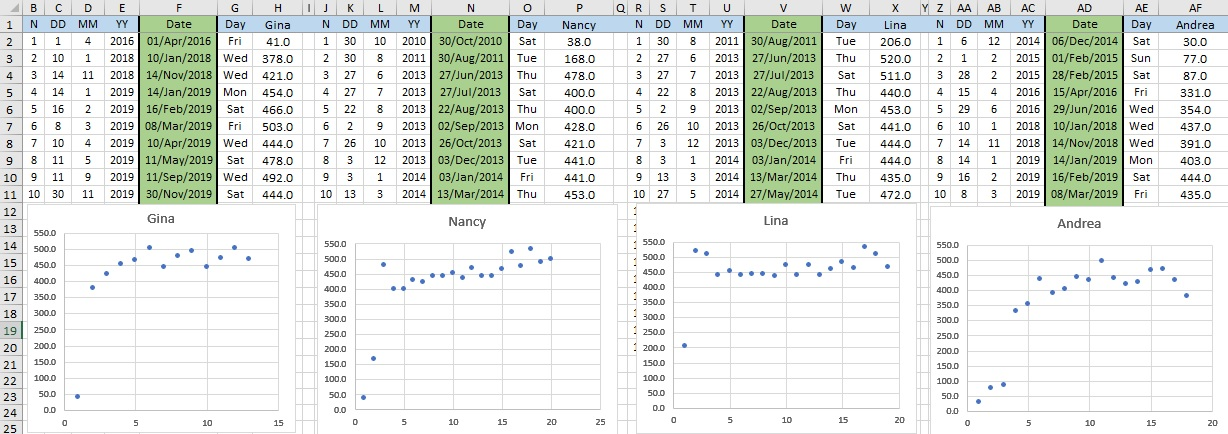
\includegraphics[scale=0.5]{img/dfinicialpeso.jpg}
	 \end{center}
	 \caption{Reorganización inicial de los datos de peso.  \label{dfpesopng}}
\end{figure}

Sin embargo, tras realizar contrastes de fechas de registros de peso con las fechas de registros de leche, se encuentra con que los registros de peso coinciden parcialmente con los registros de leche en un mismo periodo. Esto quiere decir que de los pocos datos existentes respecto al peso, estos deben ser segmentados de acuerdo con el número de parto con el que coinciden las fechas de registro de producción de leche asociadas a la lactancia de ese parto. En función de lo expresado anteriormente, se debe realizar la segmentación de los datos de peso que pertenecen a cada parto (1..6) para cada vaca perteneciente a la tabla \ref{porpartosfin} de la sección anterior.\\


\subsection{Agrupación de datos de peso}
De la tabla \ref{Nporpartos} se tienen 18 vacas diferentes para un total de 28 partos distintos que dependiendo del número de parto se cuenta con una cantidad de muestras distinta (Entre 162 y 309 muestras). Ahora bien, para los análisis algorítmicos en Matlab y/o Python, se requiere que la cantidad de muestras de leche tengan la misma cantidad de muestras para el peso en pro de lograr un análisis por ``Ecuaciones Diferenciales Ordinarias''; por tanto es necesario realizar una interpolación del(los) dato(s) de peso dependiendo de la cantidad de muestras presentes en cada parto.
%=================================================
% Please add the following required packages to your document preamble:
% \usepackage{multirow}
% \usepackage{graphicx}
% \usepackage[table,xcdraw]{xcolor}
% If you use beamer only pass "xcolor=table" option, i.e. \documentclass[xcolor=table]{beamer}
% Please add the following required packages to your document preamble:
% \usepackage{multirow}
% \usepackage{graphicx}
% \usepackage[table,xcdraw]{xcolor}
% If you use beamer only pass "xcolor=table" option, i.e. \documentclass[xcolor=table]{beamer}
\begin{table}[H]
\centering
\caption{Cantidad de muestras para cada vaca de cada parto}
\label{Nporpartos}
\resizebox{\textwidth}{!}{%
\begin{tabular}{|
>{\columncolor[HTML]{FFCE93}}c |
>{\columncolor[HTML]{C0C0C0}}c |
>{\columncolor[HTML]{A3E1F3}}c 
>{\columncolor[HTML]{A3E1F3}}c |
>{\columncolor[HTML]{A1DA8E}}c 
>{\columncolor[HTML]{A1DA8E}}c |
>{\columncolor[HTML]{FFFFC7}}c 
>{\columncolor[HTML]{FFFFC7}}c |
>{\columncolor[HTML]{F39E9E}}c |
>{\columncolor[HTML]{B791DE}}c |}
\hline
\textbf{\# de Parto} &
  \cellcolor[HTML]{343434}{\color[HTML]{FFFFFF} \textit{\textbf{1}}} &
  \multicolumn{2}{c|}{\cellcolor[HTML]{1122C6}{\color[HTML]{FFFFFF} \textit{\textbf{2}}}} &
  \multicolumn{2}{c|}{\cellcolor[HTML]{32CB00}\textit{\textbf{3}}} &
  \multicolumn{2}{c|}{\cellcolor[HTML]{FFFE65}\textit{\textbf{4}}} &
  \cellcolor[HTML]{EF3B3B}\textit{\textbf{5}} &
  \cellcolor[HTML]{AD71EB}\textit{\textbf{6}} \\ \hline
\textit{\textbf{\# de Muestras}} &
  \textbf{299} &
  \multicolumn{2}{c|}{\cellcolor[HTML]{A3E1F3}\textbf{288}} &
  \multicolumn{2}{c|}{\cellcolor[HTML]{A1DA8E}\textbf{309}} &
  \multicolumn{2}{c|}{\cellcolor[HTML]{FFFFC7}\textbf{274}} &
  \textbf{298} &
  \textbf{162} \\ \hline
\cellcolor[HTML]{FFCE93} &
  \textit{\textbf{Acerada}} &
  \multicolumn{1}{c|}{\cellcolor[HTML]{A3E1F3}\textit{\textbf{Dianita}}} &
  \textit{\textbf{Pacha}} &
  \multicolumn{1}{c|}{\cellcolor[HTML]{A1DA8E}\textit{\textbf{Fernanda}}} &
  \textit{\textbf{Martina}} &
  \multicolumn{1}{c|}{\cellcolor[HTML]{FFFFC7}\textit{\textbf{Centavito}}} &
  \textit{\textbf{Muchira}} &
  \textit{\textbf{Andrea}} &
  \textit{\textbf{Andrea}} \\ \cline{2-10} 
\cellcolor[HTML]{FFCE93} &
  \textit{\textbf{Lunita}} &
  \multicolumn{1}{c|}{\cellcolor[HTML]{A3E1F3}\textit{\textbf{Gina}}} &
  \textit{\textbf{Sol}} &
  \multicolumn{1}{c|}{\cellcolor[HTML]{A1DA8E}\textit{\textbf{Guapa}}} &
  \textit{\textbf{Morocha}} &
  \multicolumn{1}{c|}{\cellcolor[HTML]{FFFFC7}\textit{\textbf{Dianita}}} &
  \textit{\textbf{Soraya}} &
  \textit{\textbf{Guapa}} &
  \textit{\textbf{Guapa}} \\ \cline{2-10} 
\cellcolor[HTML]{FFCE93} &
  \textit{\textbf{Sol}} &
  \multicolumn{1}{c|}{\cellcolor[HTML]{A3E1F3}\textit{\textbf{Juanita}}} &
  \textit{\textbf{Viviana}} &
  \multicolumn{1}{c|}{\cellcolor[HTML]{A1DA8E}\textit{\textbf{Juanita}}} &
  \textit{\textbf{Sol}} &
  \multicolumn{1}{c|}{\cellcolor[HTML]{FFFFC7}\textit{\textbf{Leticia}}} &
  \textit{\textbf{Viviana}} &
  \textit{\textbf{}} &
  \textit{\textbf{}} \\ \cline{2-10} 
\multirow{-4}{*}{\cellcolor[HTML]{FFCE93}\textbf{\begin{tabular}[c]{@{}c@{}}Vacas \\ participantes\end{tabular}}} &
  \textit{\textbf{}} &
  \multicolumn{1}{c|}{\cellcolor[HTML]{A3E1F3}\textit{\textbf{Lucia}}} &
  \textit{\textbf{}} &
  \multicolumn{1}{c|}{\cellcolor[HTML]{A1DA8E}\textit{\textbf{Leticia}}} &
  \textit{\textbf{}} &
  \multicolumn{1}{c|}{\cellcolor[HTML]{FFFFC7}\textit{\textbf{Morocha}}} &
  \textit{\textbf{}} &
  \textit{\textbf{}} &
  \textit{\textbf{}} \\ \hline
\end{tabular}%
}
\end{table}
%=================================================

\subsubsection{Generación de columnas de peso que serán anexadas a los ``dataframes'' de cada uno de los modelos asociados al número de parto modelado}

El método usado para realizar la interpolación entre los datos de peso son las ``Splines Cúbicas'' que varían en tamaño dependiendo de la cantidad de datos presentes en cada parto. Una vez ejecutado el script de Matlab ``InterpPesosPartesEDOs'' (adjunto en este trabajo de grado)' se obtiene el conjunto de arreglos unidimensionales con los tamaños deseados (ver figura \ref{interpesospng}) y se procede a realizar la exportación correspondiente en archivos separados por comas. Posteriormente se procede a agruparlos en ``dataframes'' para su análisis por EDOs en python. Para cada lactancia se tendrá un ``dataframe'' representativo de ese modelo con las columnas de producciones de leche, peso y estiércol producido por cada vaca perteneciente a esa agrupación de lactancia.

\begin{figure}[H]
	 \begin{center}
	 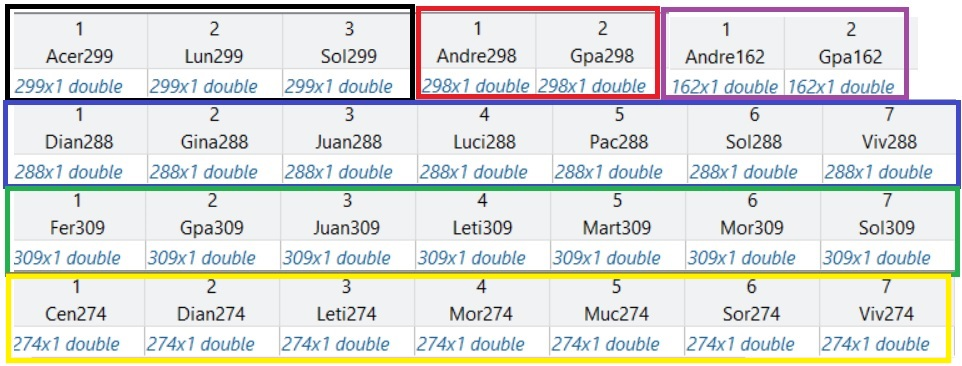
\includegraphics[scale=0.64]{img/InterPesos.jpg}
	 \end{center}
	 \caption{Formato de nombre de columna para conjunto de datos. Varia en cuanto al nombre de la vaca, cantidad de muestras existentes y cantidad de parto. El código de colores se mantiene según la tabla \ref{colorpartos} \label{interpesospng}}
\end{figure}


Llegados a este punto, ya se cuenta con los datos de las 3 variables necesarias (Producción de Leche, Estiércol, Peso) para plantear el (los) modelo(s) por EDOs, descrito en el próximo capitulo.
%================================================================================================


% \chapter{CRISP - DM: ETAPA \#3.5 - Preparación de los datos}
% 
En esta etapa, se procede a recolectar todos los datos análogos y digitales con los que cuenta en CA-SENA-POP, para almacenarlos de manera digital y proceder a analizar los datos mediante algoritmos en Matlab y/o Python. Es importante recalcar que para ambos software se requiere una estructura de datos en tablas debidamente organizadas, ya sea para tratarlos como $dataframes$, matrices, arreglos, o como tablas de archivos $^{*}.csv$.

\section{Recolección de datos} \label{datarecol}

Tal y como se mencionó en el capítulo anterior, los datos referentes a Peso, Leche y Alimentación, de cada una de las reses del CA-SENA-POP se encuentran registradas de manera física o digital; ya sea en hojas impresas como el ejemplar de la figura \ref{regleche1png}, así como también en bases de datos digitales como el de la figura \ref{tauruspng}. No obstante, estos datos \textbf{no} pueden ser importados directamente a algún software de procesamiento de datos. Esto puesto que para los datos físicos, se tienen algunas barreras y/o inconvenientes externos tales como los diferentes tipos de letra,  el estado físico de las paginas, y la diferencia entre los números de un ente registrado u otro; mientras que para los datos digitales, estos se encuentran almacenados en el software de pago de manera privada, siendo datos protegidos de acuerdo a la ley de ``Habeas data'', por lo que no pueden ser exportados directamente para manipulación del público.\\ % Feb  2023

% \subsection{Registros de ``Leche''}
Teniendo en cuenta que los datos de producción lechera se registran de manera manual, esta tarea es llevada a cabo por distintas personas. Desde aprendices hasta instructores y supervisores; por lo tanto, los datos son escritos por distintas personas, que manejan distintos tipos de letra, distinto orden, distintas practicas adecuadas de escritura, entre otras. Esto implica que los números registrados en las paginas físicas varíen de un tipo de letra a otra y deban ser analizados o copiados rigurosamente de manera digital. Además, es importante mencionar, que estas carpetas físicas de registro de datos, son expuestas a la intemperie, por lo que algunos registros han sido vulnerables ante lluvias, o sustancias que alteran el estado de la hoja de papel, dificultando así su interpretación a primera vista.\\

Es importante hacer esta observación, dado que por estas mismas circunstancias, \textbf{no} es posible extraer los datos de las tablas mediante algoritmos de inteligencia artificial de procesamiento de imágenes de manera consistente, pues estos datos pueden ser fácilmente tergiversados o malinterpretados como los ejemplares de la figura \ref{datosamanopng}.

\begin{figure}[H]
	 \begin{center}
	 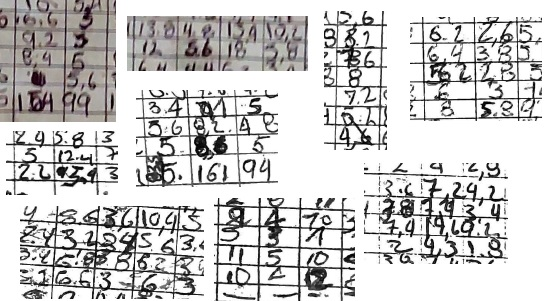
\includegraphics[scale=1.05]{img/datosamano.jpg}
	 \end{center}
	 \caption{Ejemplares de datos físicos con malas prácticas de escritura. \label{datosamanopng}}
\end{figure}

En cuanto a los registros de peso, dado que la cantidad de datos no es tan abrumadora a comparación de los registros de leche, estos datos son transcritos a archivos de excel y posteriormente a archivos con extensión $^{*}.csv$.

\section{Digitalización de los datos de producción lechera}

Teniendo en cuenta la descripción anterior, los datos fueron escaneados y posteriormente fueron transcritos de manera individual. Los datos utilizados en este trabajo consisten en los registros de producción lechera de distintas vacas que han entrado y salido de la producción ganadera, ya sea por motivos de compraventa, ingreso a gestación, salida por periodo de secado,  enfermedad, deceso, edad o cantidad de partos.\\

Los datos aquí utilizados comprenden fechas desde el 31 de Diciembre de 2018, hasta el 24 de Julio de 2022. En total se transcribieron de forma manual un total de $85.932$  datos, de los cuales, $37.956$ son datos numéricos representativos que pueden usarse para procesamiento de datos. Los $47.976$ datos restantes son datos categóricos que representan periodos de secado, horra, datos inexistentes o ilegibles, o registros desconocidos clasificados como datos NAN. Se cuenta con un total de 4 archivos pdf, en donde se almacenan los escaneos de los datos que comprenden esas fechas ya mencionadas.\\

Esta tarea de transcripción de datos tomó un tiempo aproximado de 1 semana;7 días, en jornadas de 8 horas cada día. Los datos que poseían dificultades de lectura e interpretación fueron corroborados con base en los datos de producción diaria neta y producción neta individual de cada vaca, datos existentes en las tablas escaneadas; por lo que se reduce el riesgo de transcripción de datos erróneos por causas humanas.

Aún sí existiese algún dato atípico o dato erróneo, esto puede corroborarse con la estructuración de los datos que se empleó para su análisis y que se explica en la sección a continuación.

\section{Reestructuración de los datos de leche}\label{reestructleche}
% \section{Datos de leche}
Una vez que se transcribieron los datos de manera individual para cada vaca. se procede a agrupar los datos en un archivo de excel organizado de la siguiente forma:

\subsection{Reestructuración inicial}

\begin{figure}[H]
	 \begin{center}
	 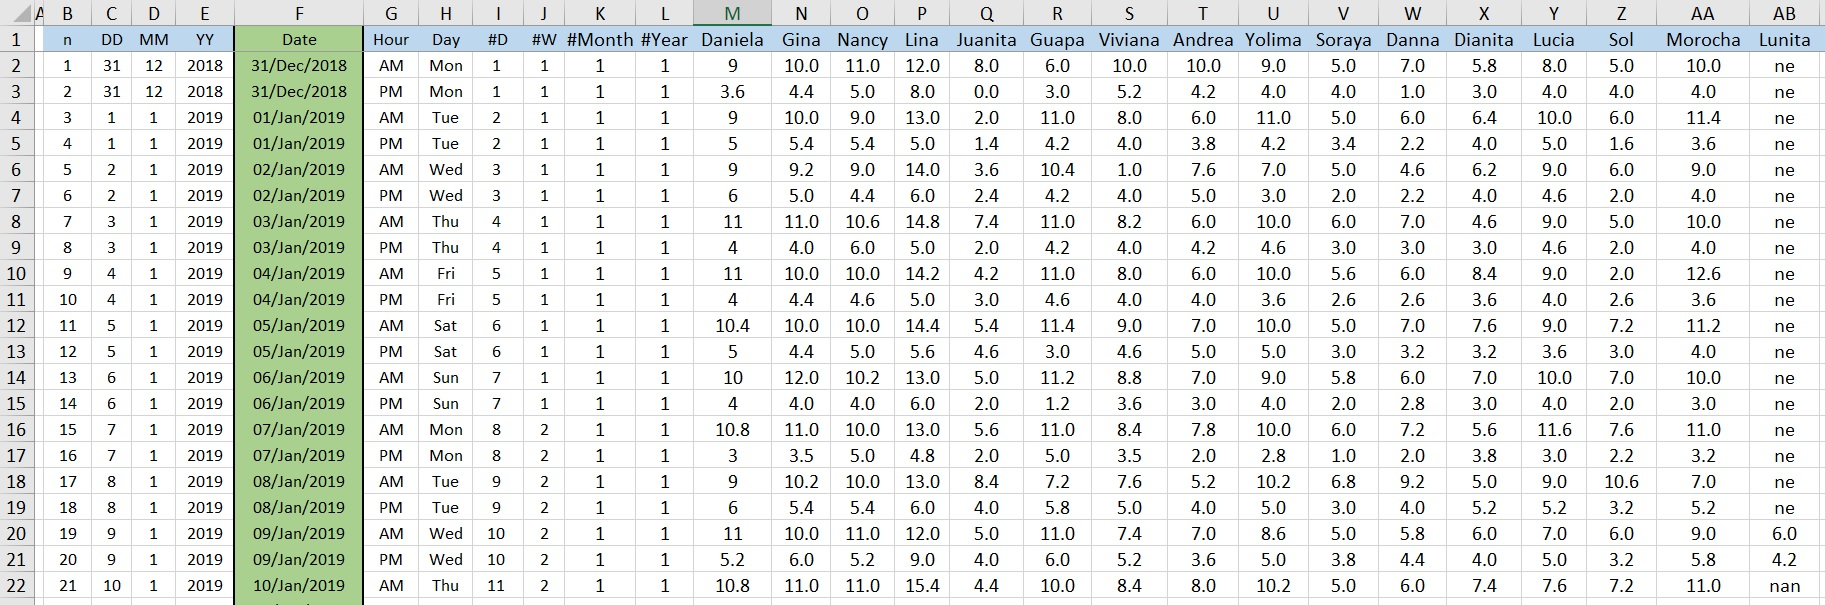
\includegraphics[scale=0.335]{img/dfinicial.jpg}
	 \end{center}
	 \caption{Reestructuración inicial de los datos de producción de leche transcritos. \label{dfinicialpng}}
\end{figure}

\begin{itemize}
    \item Cada fila, representa una \textbf{muestra - n} tomada en una \textbf{fecha (``DD/MM/AAAA'')} en una \textbf{franja horaria (AM o PM)}, en un \textbf{día de la semana (DAY y \#D)}, en una \textbf{semana (\#W)} , en un \textbf{mes (\#Month)} y en un \textbf{año (\#Year)} específico.
    \item Cada columna, representa una \textbf{vaca} que produjo una \textbf{cantidad de leche (valor numérico positivo)}.
    \item Cada 2 filas se tiene un cambio de fecha, pues se registran los datos de la mañana (AM) y también se registran los datos de la tarde (PM) como muestras separadas; más no como días distintos. Por lo tanto se tienen 2 muestras por cada día.
    \item En caso que una vaca no se encontrase en los registros de producción de leche para una fecha especifica y sus días anteriores, se cataloga como \textbf{vaca no existente} o \textbf{ne}
    \item En caso que una vaca muriera, los datos subsiguientes a esa fecha serán datos de tipo texto representados con la letra \textbf{M}.
    \item En caso que una vaca se vendiera,  los datos subsiguientes a esa fecha serán datos de tipo texto representados con la letra \textbf{V}.
    \item En caso que una vaca se encontrase en periodo de Horra,  los datos subsiguientes a esa fecha serán datos de tipo texto representados con la letra \textbf{H}, hasta indicado lo contrario.
    \item En caso que una vaca no se encontrase en periodo determinado, fuera por falta de preñes, horra, u otro motivo desconocido,  los datos subsiguientes a esa fecha aproximada serán datos de tipo texto representados con las letras \textbf{UL}, haciendo referencia a ``Unknown-Location''.
    \item En caso que una vaca se encontrase en periodo de secado, los datos subsiguientes a esa fecha serán datos de tipo texto representados con la letra \textbf{S}, hasta que se reincorpore tras el periodo de secado o hasta que se avise lo contrario (Muerte, Venta, Horra).
    \item En caso que un registro de producción de leche no haya sido transcrito, ya sea por malas practicas de escritura del documento físico, datos ilegibles o datos inexistentes, la casilla tendrá un valor de texto representado con las letras \textbf{NAN}, \textbf{haciendo referencia a un dato desconocido o dato inexistente por motivo desconocido}.
    \item En caso de tener valores numéricos 0, este valor es dejado como 0, si se muestra reincidencia en los días subsiguientes (suele suceder en fechas cercanas al periodo de secado), este valor será dejado así pues desde la práctica de toma de datos se ha considerado como una extracción de una cantidad de leche aproximadamente nula. No obstante, ya se ha mencionado que el dominio de los valores númericos de producciones de leche son \textbf{enteros positivos}.
    \item De las observaciones anteriores es importante agregar que los datos numéricos no pueden ser negativos.
    \item Se tiene un total de 2604 muestras para cada vaca, ya sea numérico o categórico. Se hace así pues las columnas de la matriz deben tener la misma cantidad de datos
    \item Se obtuvieron muestras de un total de 33 vacas distintas.
    \item Se maneja el dato desconocido con la denominación NAN y no con otro símbolo como el signo de interrogación ``?'', por motivos de formato al momento de transcribir los datos a Microsoft Excel.
\end{itemize}

\subsection{``Debugging'' y verificación de datos}

Como la transcripción de los datos se realiza de forma manual, existe el riesgo de añadir error humano a mediciones que ya cuentan con errores de medición y escritura. Para disminuir este error de transcripción, se verificó uno a uno los valores, antes, durante y después del proceso de transcripción. No obstante puede que se hayan pasado valores por alto como reflejo de un error humano.\\

Para ello, una vez obtenida la matriz agrupada en Excel, se verifican los tipos de datos y se corrobora que la cantidad neta de cada grupo sumen la cantidad total de datos. En caso contrario, el valor en cuestión se puede identificar el índice de la(s) muestra(s) no identificada(s) y mediante la fecha en la que fue(ron)  tomada(s), se puede corroborar tanto en la tabla de Excel, como en los archivos pdf escaneados. 

\subsection{Reestructuración numérica}

Notese que en la reestructuración inicial se puede observar que los datos pueden ser numéricos o categóricos, no obstante esto dificulta su análisis matricial en el software de Matlab por lo que se procede a tener algunas consideraciones adicionales.

\begin{itemize}
    \item En caso de muerte o venta, se considera como dato de valor numérico 0.0, pues se considera como una producción de leche nula dado que no se puede extraer leche de un animal muerto o vendido, mas no obstante, no es considerado como valor de tipo NAN, \textbf{pues se considera NAN un valor que no pudo ser medido y se desconoce el motivo.}
    \item Como los datos no pueden ser biológica ni físicamente negativos; en caso que una vaca no existiese en fechas anteriores a la fecha de registro (los datos \textbf{ne}), se cambiará el valor categórico \textbf{ne} por un \textbf{-1}.
\end{itemize}


Así pues, se conforma un primer archivo de excel con todos los registros existentes hasta la fecha del 24 de Julio del 2022. Es importante mencionar que el balance existente entre datos numéricos útiles para procesamiento y análisis, con datos de tipo NAN es  aproximadamente de 90\% contra menos del 10\% respectivamente. Y en comparación de datos de tipo NAN con datos conocidos, ya sean numéricos representativos o datos categóricos transformados; el porcentaje de balance disminuye hasta un 5.6\%.\\

De esta manera se puede considerar que los datos de tipo NAN no son significativos para los análisis posteriores, y pueden pasarse por alto o reemplazarse con métodos de imputación, sin afectar negativamente los análisis a futuro.
% se puede corroborar en DATAF SENA 2022 AGO 21 DATA RAW NUM - SUPER VACA

\pagebreak

\subsection{Clasificación, Selección y Agrupación de datos de leche}
Teniendo en cuenta la base de datos estructurada en el punto anterior, es importante cuestionarse sí estos datos pueden representar matemáticamente toda la producción de leche del CA-SENA-POP, pues aunque son datos que evidencian la producción neta de la granja, estos datos dispersos no permiten una aproximación mediante funciones y/o modelos matemáticos, ni mucho menos posibilitan el modelamiento dinámico mediante ecuaciones diferenciales. Por lo tanto es imprescindible estimar una o varias funciones que representen de manera aproximada, los datos obtenidos.\\

Es decir, que se debe considerar un ajuste de curvas a los datos existentes para aproximar la producción neta mediante funciones y modelos matemáticos. Por otra parte es importante tener en cuenta que las producciones de leche de cada animal, varían según el número de partos que hayan experimentado con anterioridad. Las vacas primíparas que recién están produciendo leche, no tendrán un rendimiento equiparable a comparación de las vacas que ya se encuentran en un 3er o 4to parto; en consecuencia es plausible realizar una clasificación de vacas por su cantidad de partos y observar el comportamiento de las producciones lecheras para cada grupo de partos.\\

\subsubsection{Clasificación de Datos}

Así pues, con base en las observaciones anteriores y partiendo de los datos existentes del CA-SENA-POP, tendremos 6 grupos distintos de partos. $Parto_{i}$, con i=1...6\\

Notese que los datos previamente estructurados cuentan con los registros de producción lechera desde el año 2018 hasta el año 2022, con todos los registros existentes para cada una de las vacas. No obstante, en este periodo de tiempo, en los documentos físicos no se específica el número de parto de cada animal. En algunos casos se ha hecho la observación, mas sin embargo no aplica para todas las reses. Observese además, que los partos entre las vacas no están sincronizados; por lo que esta clasificación permite identificar qué vacas son contemporáneas con otras. Por ende, es necesario acudir a la base de datos digital del software TaurusWebs con el que cuenta el centro agropecuario; para hacer una validación cruzada de los datos.\\

Una vez obtenido el permiso y una copia de la base de datos actual, suministrada por el encargado Daniel Cobo. se puede acceder al software con una versión gratuita de prueba; licencia que satisface la posibilidad de consultar las fechas de parto de cada bovino. Esto se logra gracias a la trazabilidad con la que cuenta este software y se puede hacer contraste con los datos previamente estructurados; dándose la posibilidad de clasificar los datos según el parto al que corresponden para cada ternera:

\begin{figure}[H]
	 \begin{center}
	 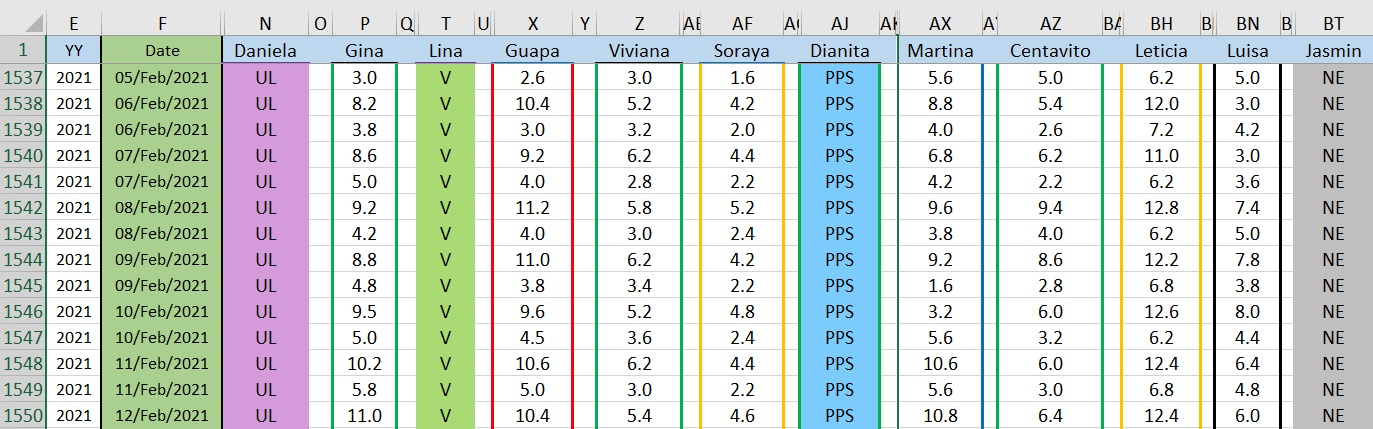
\includegraphics[scale=0.45]{img/dfcolorpartos.jpg}
	 \end{center}
	 \caption{Clasificación de datos por \#Parto para cada vaca. \label{colorpartospng}}
\end{figure}

En la figura anterior se puede observar que la clasificación de los partos se realiza con base en la estructuración de datos tanto categóricos como numéricos. Esto con el objetivo de diferenciar de manera visual entre un periodo de producción de leche a un periodo de secado (Casilla blanca con borde de color y casillas coloreadas de color azul respectivamente). No obstante una vez realizada la clasificación, selección y agrupación de datos; las matrices usadas en los análisis posteriores con algoritmos en Matlab, manejan la estructuración numérica descrita en la sub-sección anterior.\\

Percatese que al tener 6 grupos de partos en el CA-SENA-POP, se utiliza un código de colores para la clasificación de producción por \# de Parto, siendo esta la siguiente:

% Please add the following required packages to your document preamble:
% \usepackage{graphicx}
% \usepackage[table,xcdraw]{xcolor}
% If you use beamer only pass "xcolor=table" option, i.e. \documentclass[xcolor=table]{beamer}
\begin{table}[H]
\centering
\caption{Código de colores por número de parto}
\label{colorpartos}
\resizebox{\textwidth}{!}{%
\begin{tabular}{|
>{\columncolor[HTML]{FFCE93}}c |
>{\columncolor[HTML]{000000}}c |
>{\columncolor[HTML]{1122C6}}c |
>{\columncolor[HTML]{32CB00}}c |
>{\columncolor[HTML]{FFFE65}}c |
>{\columncolor[HTML]{EF3B3B}}c |
>{\columncolor[HTML]{AD71EB}}c |}
\hline
\textit{\textbf{\begin{tabular}[c]{@{}c@{}}Color del\\  borde\end{tabular}}} &
  {\color[HTML]{FFFFFF} \textit{\textbf{Negro}}} &
  {\color[HTML]{FFFFFF} \textit{\textbf{Azul}}} &
  \textit{\textbf{Verde}} &
  \textit{\textbf{Amarillo}} &
  \textit{\textbf{Rojo}} &
  \textit{\textbf{Morado}} \\ \hline
\textit{\textbf{\begin{tabular}[c]{@{}c@{}}\# de \\ Parto\end{tabular}}} &
  \cellcolor[HTML]{C0C0C0}\textit{\textbf{1}} &
  \cellcolor[HTML]{A3E1F3}\textit{\textbf{2}} &
  \cellcolor[HTML]{A1DA8E}\textit{\textbf{3}} &
  \cellcolor[HTML]{FFFFC7}\textit{\textbf{4}} &
  \cellcolor[HTML]{F39E9E}\textit{\textbf{5}} &
  \cellcolor[HTML]{B791DE}\textit{\textbf{6}} \\ \hline
\end{tabular}%
}
\end{table}

Así pues, se obtienen 6 grupos de un tamaño variable de vacas para cada número de parto. Esta clasificación se puede observar en la tabla \ref{porpartos}. % la tabla gigante de colores que no se deja poner label

\subsubsection{Selección de Datos}

Una de las primeras observaciones obtenidas al realizar la agrupación por partos; es que los datos existentes que han sido agrupados no poseen igual cantidad de datos para cada res. Esto se produce dado que los partos varían en cuestión de duración para cada animal. En primera instancia esto no debería suponer un problema significativo, pues en caso que los partos posean una ligera variabilidad de muestras; bastaría con ``rellenar'' los datos faltantes con ceros o con imputación de datos como la media o la moda; ó por otra parte, bastaría con realizar una agrupación con igual cantidad de muestras.\\

Sin embargo, esta contra medida no puede ser llevada a cabo en razón de que los datos existentes facilitan la agrupación por partos, mas no garantiza que los datos de un parto en específico se encuentren disponibles en su totalidad. En otras palabras, muchos de los datos que se tienen para cada parto son datos de inicio de producción o finalización de producción de leche de las terneras, tanto para las que fallecen, para las que se venden, así como también, para las que a fecha del 31 de Diciembre del 2018 ya se encontraban en periodo productivo.\\

Si se realiza una representación visual individual de los datos, se puede observar claramente que algunas reses tienen muy pocos datos, lo que ``recargaría'' la distribución hacia los extremos, dificultando su análisis descriptivo. Por otra parte, si se hace un contraste de datos teniendo como punto de referencia el inicio de la producción o su finalización en el periodo de secado, la tabla de registros permite evidenciar el desbalance que manifiestan los datos:

\begin{figure}[H]
	 \begin{center}
	 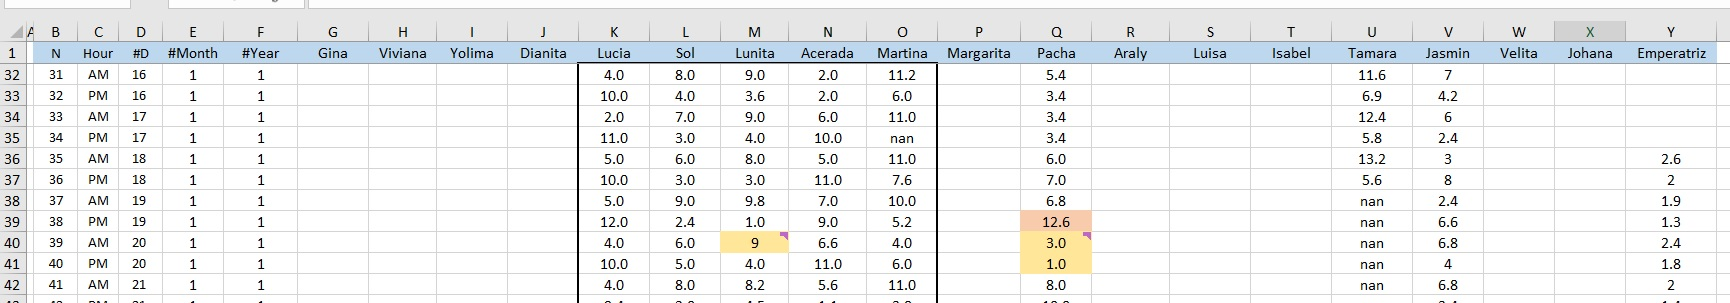
\includegraphics[scale=0.34]{img/partosincompletos.jpg}
	 \end{center}
	 \caption{Desbalance de datos en agrupación inicial por partos. \label{partosincompletospng}}
\end{figure}

En la figura anterior, se evidencia claramente el desbalance mencionado. Si se observan mas a fondo los datos presentes en el archivo de Excel; 13 de las 19 reses cuentan con menos de la mitad de muestras de producción lechera tras haber parido por primera vez. Solo una de ellas, manifiesta un exceso de registros antes de entrar en periodo de secado; y 5 mamíferos restantes aparentan tener la cantidad de muestras suficientes para representar el grupo de vacas primíparas. Las 5 vacas en cuestión son ``Lucia'', ``Sol'', ``Lunita'', ``Acerada'' y ``Martina''.\\

Finalmente, aunque todas las reses cuentan con la misma cantidad de datos, se procede a seleccionar únicamente a 3 de ellas que coinciden en el inicio y finalización de la producción de leche (``Sol'', ``Lunita'', ``Acerada''). Mientras que las otras 2; a pesar de tener la misma cantidad de muestras, presentan desfases en el inicio y finalización de la etapa productiva (Lucia y Martina). De esta forma, se puede generar la primera representación visual de los datos mediante un gráfico de dispersión, tal y como se observa en la  figura \ref{scatterparto1png}.

\begin{figure}[H]
	 \begin{center}
	 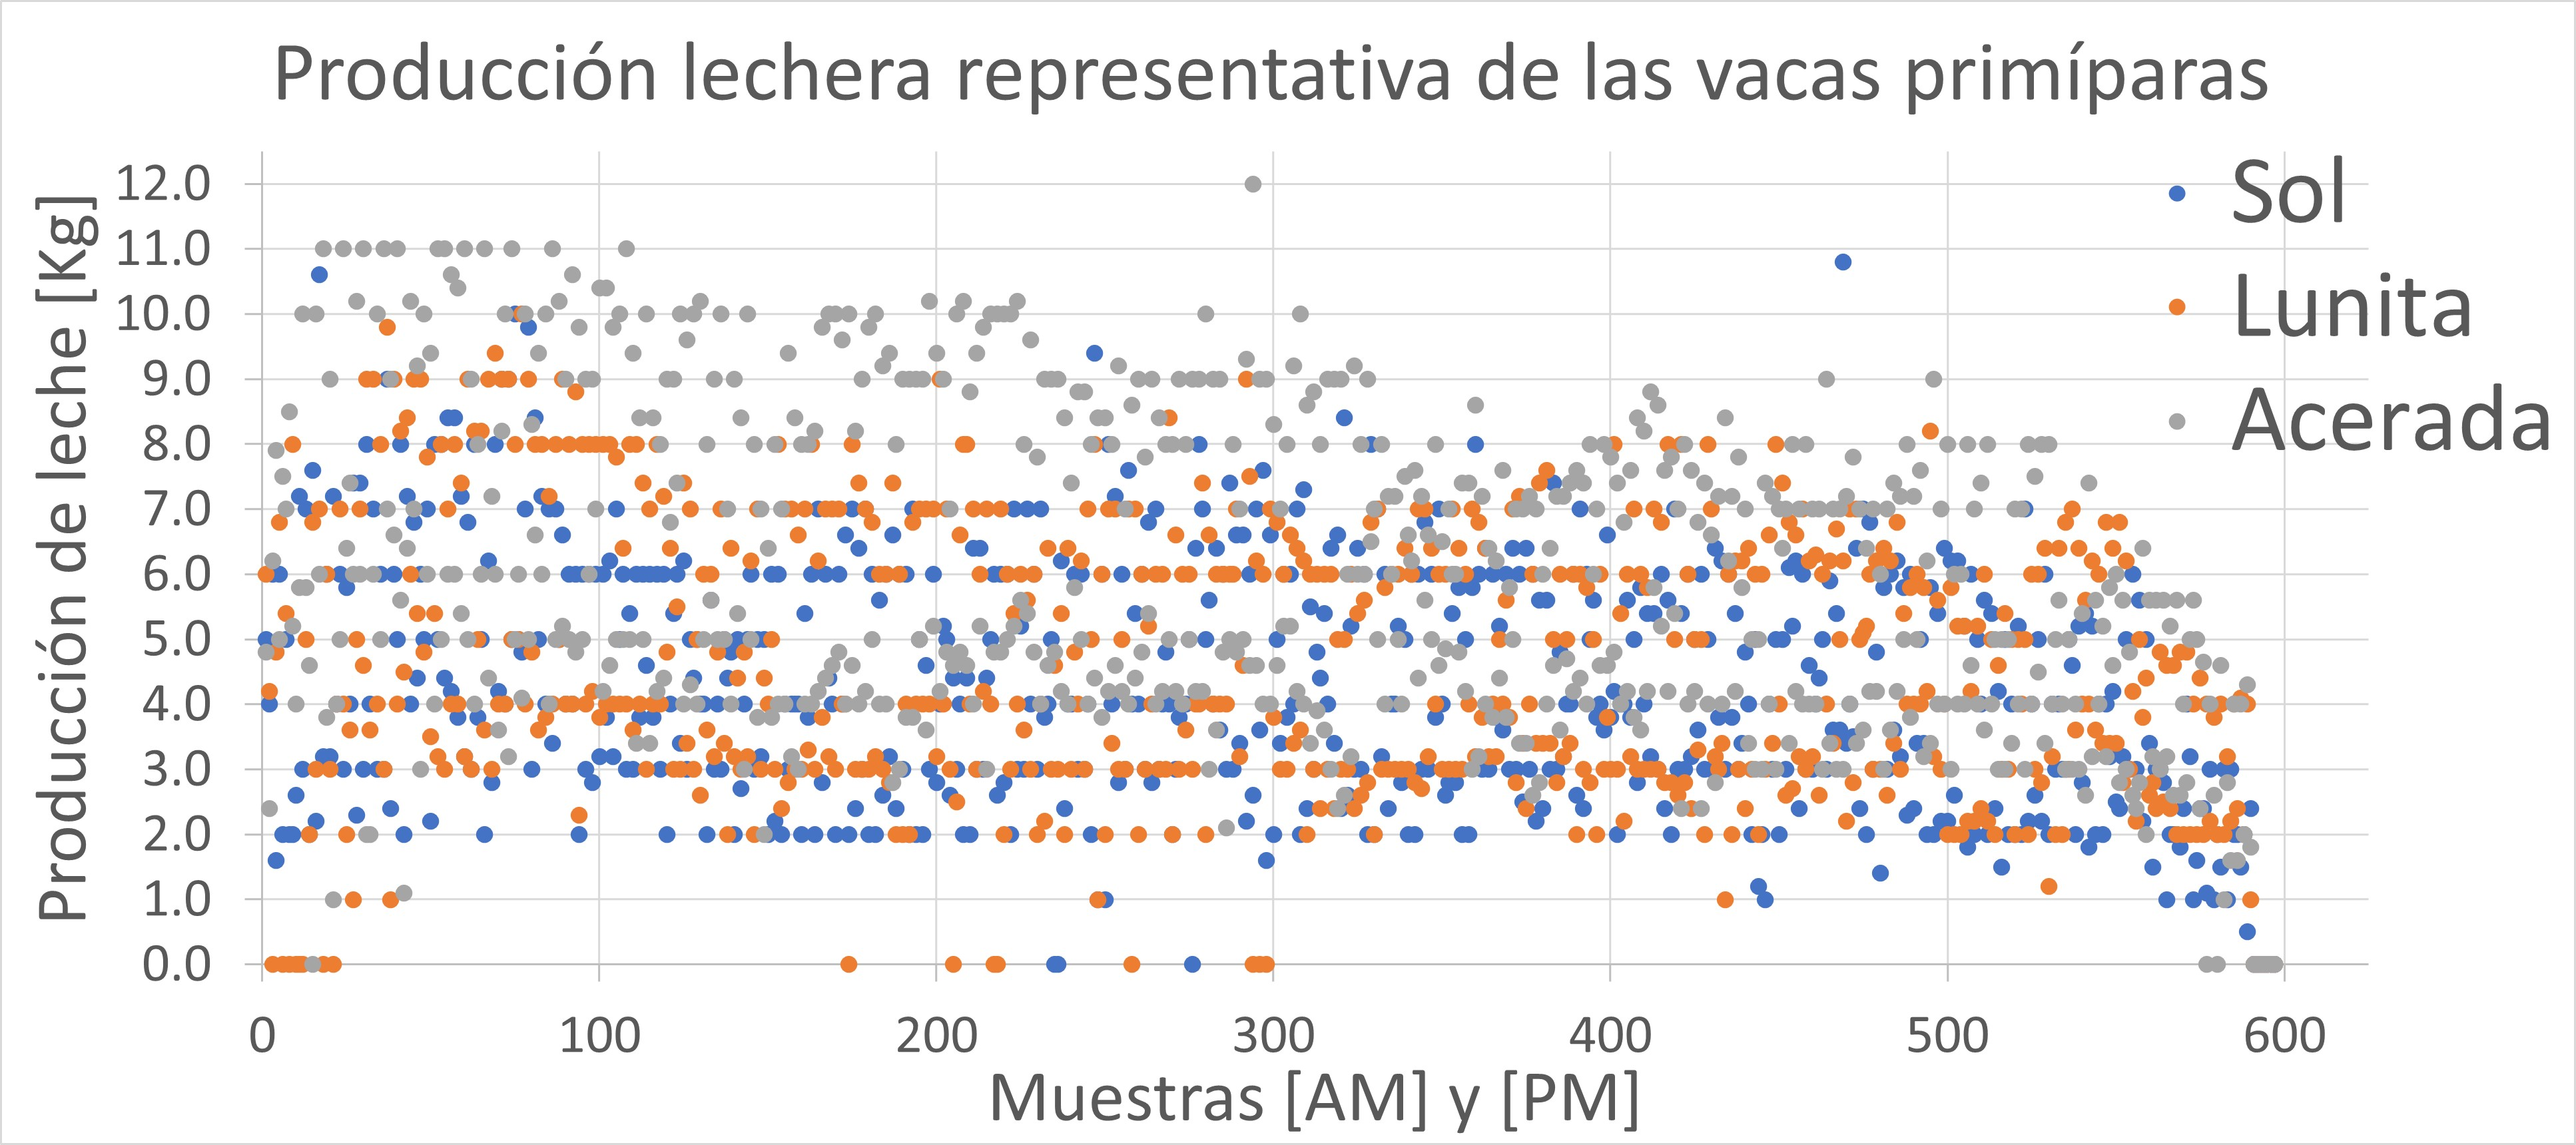
\includegraphics[scale=0.452]{img/scatterparto1.jpg}
	 \end{center}
	 \caption{Gráfico de dispersión para representar la producción lechera de las vacas primíparas. \label{scatterparto1png}}
\end{figure}

\subsubsection{Agrupación de Datos}

El resultado obtenido tras realizar la primer representación visual de datos da un idea de cómo no se deben utilizar los datos para los análisis matemáticos. Pues se observa que al tener muestras matutinas y vespertinas juntas, no se logran diferenciar los datos correspondientes a cada intervalo. Además, el intervalo de tiempo es de 305 días aproximadamente y al manejar ambos tipos de muestras, se tiene un total de 610 datos en el eje horizontal. Por ende, como medida inicial, se opta por realizar un análisis independiente para las muestras obtenidas en diferentes horas del día, procediendo con una representación individual como se observa a continuación:

\begin{figure}[H]
	 \begin{center}
	 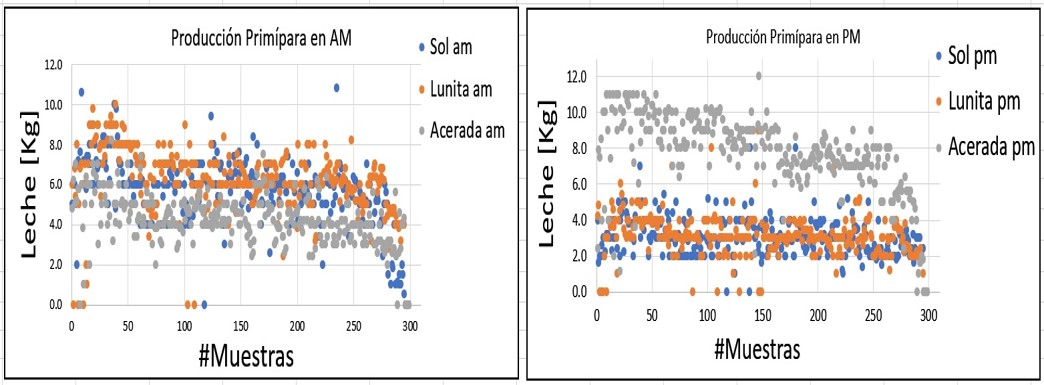
\includegraphics[scale=0.575]{img/desfaseAMPM.jpg}
	 \end{center}
	 \caption{Gráfico de dispersión para Muestras matutinas y vespertinas. \label{desfaseAMPMpng}}
\end{figure}

En primera instancia parece que la gráfica anterior no presenta ningún inconveniente, a pesar de ello, se puede notar un leve desajuste entre los valores vespertinos; pues los valores de la res denominada como ``Acerada'', muestran una lejanía con los otros datos en el horario de la tarde. Esto genera ciertas inquietudes teniendo en cuenta que las muestras matutinas tienden a ser mayores que las muestras vespertinas para la mayoría de las reses de este estudio. En virtud de que el lapso que existe entre una muestra matutina con una vespertina en un mismo día es de aproximadamente 10 horas; mientras que el lapso entre una muestra vespertina y una muestra matutina es de aproximadamente 14 horas; no sería de extrañar que al tener mayor tiempo de recuperación, se le pueda extraer mayor cantidad de leche a la vaca.

Lo anterior se presta para realizar nuevamente una corroboración de los datos con los datos manuales existentes y la tabla de datos de la estructuración inicial; con lo que se observa que al realizar la ``alineación'' de datos tras la agrupación por partos; los datos matutinos de la res en cuestión han quedado ``alineados'' con los datos vespertinos de las otras reses. Esto quiere decir que la figura \ref{desfaseAMPMpng} debe cambiarse por la figura \ref{AMPMsindesfasepng}:


\begin{figure}[H]
	 \begin{center}
	 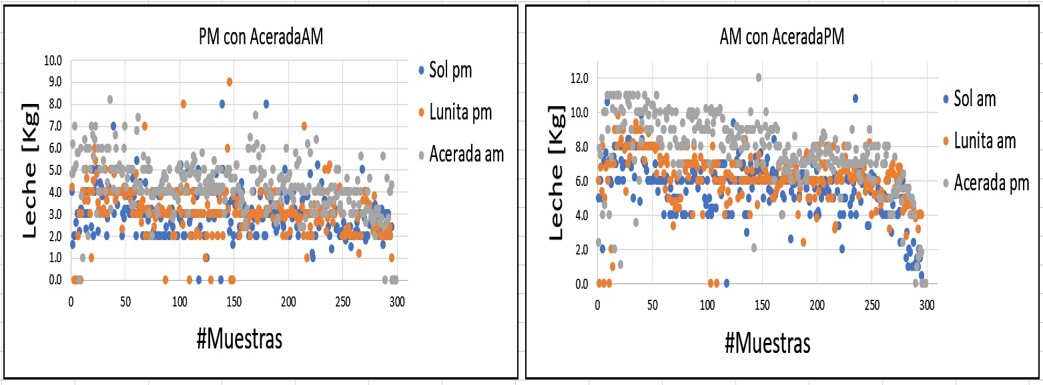
\includegraphics[scale=0.5835]{img/AMPMsindesfase.jpg}
	 \end{center}
	 \caption{Gráfico de dispersión para Muestras matutinas y vespertinas. \label{AMPMsindesfasepng}}
\end{figure}


De acuerdo con la situación anterior, se concluye que realizar un análisis por franja horaria puede llevar a errores futuros o a reincidentes corroboraciones de datos, siendo esto último una tarea agobiante para el caso de estudio; por lo que se decide considerar únicamente análisis con la producción neta diaria de cada animal. De esta forma se repite el proceso para los otros grupos de partos obteniéndose los gráficos de dispersión de la figura \ref{svnetaspng} y obteniéndose un conjunto total de 28 reses para análisis futuros; que se puede observar en la tabla \ref{porpartosfin}.

% Please add the following required packages to your document preamble:
% \usepackage{multirow}
% \usepackage{graphicx}
% \usepackage[table,xcdraw]{xcolor}
% If you use beamer only pass "xcolor=table" option, i.e. \documentclass[xcolor=table]{beamer}
%=======================================================
% Please add the following required packages to your document preamble:
% \usepackage{multirow}
% \usepackage{graphicx}
% \usepackage[table,xcdraw]{xcolor}
% If you use beamer only pass "xcolor=table" option, i.e. \documentclass[xcolor=table]{beamer}
% Please add the following required packages to your document preamble:
% \usepackage{multirow}
% \usepackage{graphicx}
% \usepackage[table,xcdraw]{xcolor}
% If you use beamer only pass "xcolor=table" option, i.e. \documentclass[xcolor=table]{beamer}
\begin{table}[H]
\centering
\caption{Agrupación final de vacas por \# de partos}
\label{porpartosfin}
\resizebox{\textwidth}{!}{%
\begin{tabular}{|
>{\columncolor[HTML]{FFCE93}}c |
>{\columncolor[HTML]{C0C0C0}}c |
>{\columncolor[HTML]{A3E1F3}}c 
>{\columncolor[HTML]{A3E1F3}}c |
>{\columncolor[HTML]{A1DA8E}}c 
>{\columncolor[HTML]{A1DA8E}}c |
>{\columncolor[HTML]{FFFFC7}}c 
>{\columncolor[HTML]{FFFFC7}}c |
>{\columncolor[HTML]{F39E9E}}c |
>{\columncolor[HTML]{B791DE}}c |}
\hline
\textit{\textbf{\# de Parto}} &
  \cellcolor[HTML]{000000}{\color[HTML]{FFFFFF} \textit{\textbf{1}}} &
  \multicolumn{2}{c|}{\cellcolor[HTML]{1122C6}{\color[HTML]{FFFFFF} \textit{\textbf{2}}}} &
  \multicolumn{2}{c|}{\cellcolor[HTML]{32CB00}\textit{\textbf{3}}} &
  \multicolumn{2}{c|}{\cellcolor[HTML]{FFFE65}\textit{\textbf{4}}} &
  \cellcolor[HTML]{EF3B3B}\textit{\textbf{5}} &
  \cellcolor[HTML]{AD71EB}\textit{\textbf{6}} \\ \hline
\cellcolor[HTML]{FFCE93} &
  \textit{\textbf{Acerada}} &
  \multicolumn{1}{c|}{\cellcolor[HTML]{A3E1F3}\textit{\textbf{Dianita}}} &
  \textit{\textbf{Pacha}} &
  \multicolumn{1}{c|}{\cellcolor[HTML]{A1DA8E}\textit{\textbf{Fernanda}}} &
  \textit{\textbf{Martina}} &
  \multicolumn{1}{c|}{\cellcolor[HTML]{FFFFC7}\textit{\textbf{Centavito}}} &
  \textit{\textbf{Muchira}} &
  \textit{\textbf{Andrea}} &
  \textit{\textbf{Andrea}} \\ \cline{2-10} 
\cellcolor[HTML]{FFCE93} &
  \textit{\textbf{Lunita}} &
  \multicolumn{1}{c|}{\cellcolor[HTML]{A3E1F3}\textit{\textbf{Gina}}} &
  \textit{\textbf{Sol}} &
  \multicolumn{1}{c|}{\cellcolor[HTML]{A1DA8E}\textit{\textbf{Guapa}}} &
  \textit{\textbf{Morocha}} &
  \multicolumn{1}{c|}{\cellcolor[HTML]{FFFFC7}\textit{\textbf{Dianita}}} &
  \textit{\textbf{Soraya}} &
  \textit{\textbf{Guapa}} &
  \textit{\textbf{Guapa}} \\ \cline{2-10} 
\cellcolor[HTML]{FFCE93} &
  \textit{\textbf{Sol}} &
  \multicolumn{1}{c|}{\cellcolor[HTML]{A3E1F3}\textit{\textbf{Juanita}}} &
  \textit{\textbf{Viviana}} &
  \multicolumn{1}{c|}{\cellcolor[HTML]{A1DA8E}\textit{\textbf{Juanita}}} &
  \textit{\textbf{Sol}} &
  \multicolumn{1}{c|}{\cellcolor[HTML]{FFFFC7}\textit{\textbf{Leticia}}} &
  \textit{\textbf{Viviana}} &
  \textit{\textbf{}} &
  \textit{\textbf{}} \\ \cline{2-10} 
\multirow{-4}{*}{\cellcolor[HTML]{FFCE93}\textit{\textbf{\begin{tabular}[c]{@{}c@{}}Vacas \\ participantes\end{tabular}}}} &
  \textit{\textbf{}} &
  \multicolumn{1}{c|}{\cellcolor[HTML]{A3E1F3}\textit{\textbf{Lucia}}} &
  \textit{\textbf{}} &
  \multicolumn{1}{c|}{\cellcolor[HTML]{A1DA8E}\textit{\textbf{Leticia}}} &
  \textit{\textbf{}} &
  \multicolumn{1}{c|}{\cellcolor[HTML]{FFFFC7}\textit{\textbf{Morocha}}} &
  \textit{\textbf{}} &
  \textit{\textbf{}} &
  \textit{\textbf{}} \\ \hline
\end{tabular}%
}
\end{table}
%=======================================================
% Corregir que el parto 4 no salió bien la leyenda >:C

\begin{figure}[H]
	 \begin{center}
	 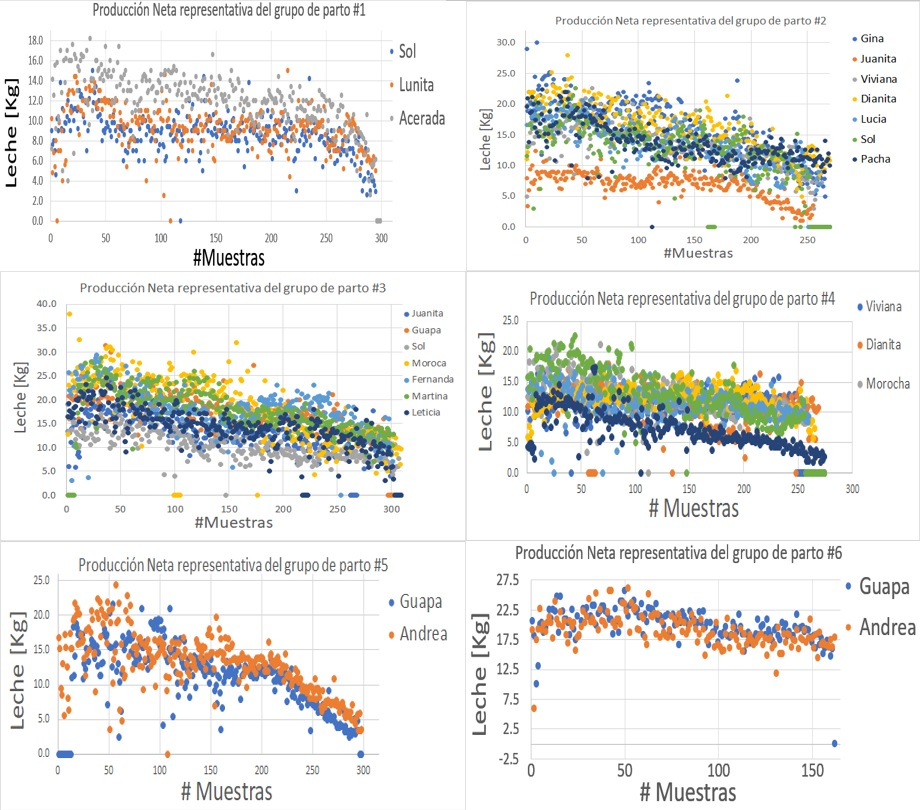
\includegraphics[scale=0.675]{img/svnetas.jpg}
	 \end{center}
	 \caption{Gráfico de dispersión para cada grupo de partos. \label{svnetaspng}}
\end{figure}


% , dando paso en este análisis, que la agrupación de datos de dispersión por partos se le denomine como datos de dispersión neta de ``supervaca'' del parto 1:

% \begin{figure}[H]
% 	 \begin{center}
% 	 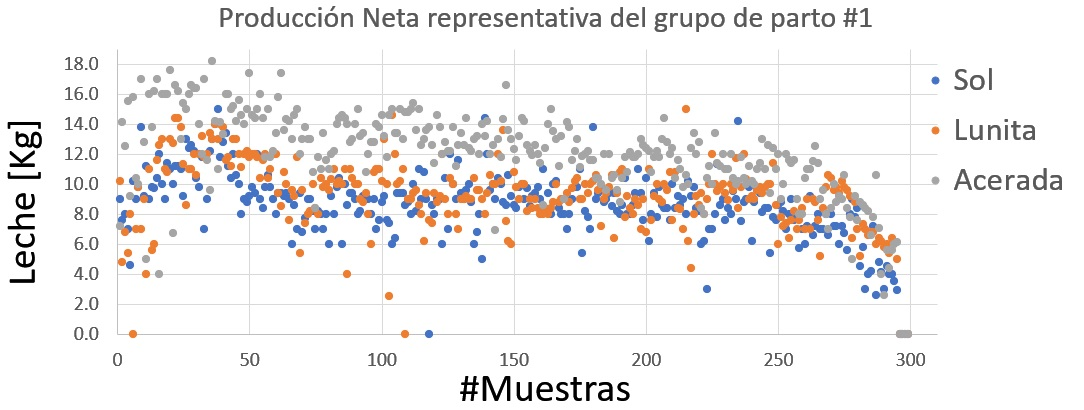
\includegraphics[scale=0.6]{img/svnetap1.jpg}
% 	 \end{center}
% 	 \caption{Gráfico de dispersión para registros de producción neta en vacas primíparas . \label{desfaseAMPMpng}}
% \end{figure}

%================================================================================================
% Please add the following required packages to your document preamble:
% \usepackage{multirow}
% \usepackage{graphicx}
% \usepackage[table,xcdraw]{xcolor}
% If you use beamer only pass "xcolor=table" option, i.e. \documentclass[xcolor=table]{beamer}
% Please add the following required packages to your document preamble:
% \usepackage{multirow}
% \usepackage{graphicx}
% \usepackage[table,xcdraw]{xcolor}
% If you use beamer only pass "xcolor=table" option, i.e. \documentclass[xcolor=table]{beamer}
\begin{table}[H]
\centering
\caption{Agrupación de vacas por \# de partos}
\label{porpartos}
\resizebox{\textwidth}{!}{%
\begin{tabular}{|c|ccccc|}
\hline
\rowcolor[HTML]{FFCE93} 
\textit{\textbf{\begin{tabular}[c]{@{}c@{}}\# de \\ Parto\end{tabular}}} &
  \multicolumn{5}{c|}{\cellcolor[HTML]{FFCE93}\textit{\textbf{\begin{tabular}[c]{@{}c@{}}Vacas \\ participantes\end{tabular}}}} \\ \hline
\rowcolor[HTML]{C0C0C0} 
\cellcolor[HTML]{000000}{\color[HTML]{FFFFFF} } &
  \multicolumn{1}{c|}{\cellcolor[HTML]{C0C0C0}\textit{\textbf{Gina}}} &
  \multicolumn{1}{c|}{\cellcolor[HTML]{C0C0C0}\textit{\textbf{Viviana}}} &
  \multicolumn{1}{c|}{\cellcolor[HTML]{C0C0C0}\textit{\textbf{Yolima}}} &
  \multicolumn{1}{c|}{\cellcolor[HTML]{C0C0C0}\textit{\textbf{Dianita}}} &
  \textit{\textbf{Lucia}} \\ \cline{2-6} 
\rowcolor[HTML]{C0C0C0} 
\cellcolor[HTML]{000000}{\color[HTML]{FFFFFF} } &
  \multicolumn{1}{c|}{\cellcolor[HTML]{C0C0C0}\textit{\textbf{Pacha}}} &
  \multicolumn{1}{c|}{\cellcolor[HTML]{C0C0C0}\textit{\textbf{Araly}}} &
  \multicolumn{1}{c|}{\cellcolor[HTML]{C0C0C0}\textit{\textbf{Luisa}}} &
  \multicolumn{1}{c|}{\cellcolor[HTML]{C0C0C0}\textit{\textbf{Isabel}}} &
  \textit{\textbf{Tamara}} \\ \cline{2-6} 
\rowcolor[HTML]{C0C0C0} 
\cellcolor[HTML]{000000}{\color[HTML]{FFFFFF} } &
  \multicolumn{1}{c|}{\cellcolor[HTML]{C0C0C0}\textit{\textbf{Sol}}} &
  \multicolumn{1}{c|}{\cellcolor[HTML]{C0C0C0}\textit{\textbf{Lunita}}} &
  \multicolumn{1}{c|}{\cellcolor[HTML]{C0C0C0}\textit{\textbf{Acerada}}} &
  \multicolumn{1}{c|}{\cellcolor[HTML]{C0C0C0}\textit{\textbf{Martina}}} &
  \textit{\textbf{Margarita}} \\ \cline{2-6} 
\rowcolor[HTML]{C0C0C0} 
\multirow{-4}{*}{\cellcolor[HTML]{000000}{\color[HTML]{FFFFFF} \textit{\textbf{1}}}} &
  \multicolumn{1}{c|}{\cellcolor[HTML]{C0C0C0}\textit{\textbf{Jasmin}}} &
  \multicolumn{1}{c|}{\cellcolor[HTML]{C0C0C0}\textit{\textbf{Velita}}} &
  \multicolumn{1}{c|}{\cellcolor[HTML]{C0C0C0}\textit{\textbf{Johana}}} &
  \multicolumn{1}{c|}{\cellcolor[HTML]{C0C0C0}\textit{\textbf{Emperatriz}}} &
  \textit{\textbf{}} \\ \hline
\rowcolor[HTML]{A3E1F3} 
\cellcolor[HTML]{1122C6}{\color[HTML]{FFFFFF} } &
  \multicolumn{1}{c|}{\cellcolor[HTML]{A3E1F3}\textit{\textbf{Gina}}} &
  \multicolumn{1}{c|}{\cellcolor[HTML]{A3E1F3}\textit{\textbf{Juanita}}} &
  \multicolumn{1}{c|}{\cellcolor[HTML]{A3E1F3}\textit{\textbf{Guapa}}} &
  \multicolumn{1}{c|}{\cellcolor[HTML]{A3E1F3}\textit{\textbf{Viviana}}} &
  \textit{\textbf{}} \\ \cline{2-6} 
\rowcolor[HTML]{A3E1F3} 
\cellcolor[HTML]{1122C6}{\color[HTML]{FFFFFF} } &
  \multicolumn{1}{c|}{\cellcolor[HTML]{A3E1F3}\textit{\textbf{Fernanda}}} &
  \multicolumn{1}{c|}{\cellcolor[HTML]{A3E1F3}\textit{\textbf{Acerada}}} &
  \multicolumn{1}{c|}{\cellcolor[HTML]{A3E1F3}\textit{\textbf{Martina}}} &
  \multicolumn{1}{c|}{\cellcolor[HTML]{A3E1F3}\textit{\textbf{Centavito}}} &
  \textit{\textbf{}} \\ \cline{2-6} 
\rowcolor[HTML]{A3E1F3} 
\cellcolor[HTML]{1122C6}{\color[HTML]{FFFFFF} } &
  \multicolumn{1}{c|}{\cellcolor[HTML]{A3E1F3}\textit{\textbf{Andrea}}} &
  \multicolumn{1}{c|}{\cellcolor[HTML]{A3E1F3}\textit{\textbf{Yolima}}} &
  \multicolumn{1}{c|}{\cellcolor[HTML]{A3E1F3}\textit{\textbf{Soraya}}} &
  \multicolumn{1}{c|}{\cellcolor[HTML]{A3E1F3}\textit{\textbf{Danna}}} &
  \textit{\textbf{}} \\ \cline{2-6} 
\rowcolor[HTML]{A3E1F3} 
\cellcolor[HTML]{1122C6}{\color[HTML]{FFFFFF} } &
  \multicolumn{1}{c|}{\cellcolor[HTML]{A3E1F3}\textit{\textbf{Muchira}}} &
  \multicolumn{1}{c|}{\cellcolor[HTML]{A3E1F3}\textit{\textbf{Margarita}}} &
  \multicolumn{1}{c|}{\cellcolor[HTML]{A3E1F3}\textit{\textbf{Romina}}} &
  \multicolumn{1}{c|}{\cellcolor[HTML]{A3E1F3}\textit{\textbf{Pacha}}} &
  \textit{\textbf{}} \\ \cline{2-6} 
\rowcolor[HTML]{A3E1F3} 
\cellcolor[HTML]{1122C6}{\color[HTML]{FFFFFF} } &
  \multicolumn{1}{c|}{\cellcolor[HTML]{A3E1F3}\textit{\textbf{Dianita}}} &
  \multicolumn{1}{c|}{\cellcolor[HTML]{A3E1F3}\textit{\textbf{Lucia}}} &
  \multicolumn{1}{c|}{\cellcolor[HTML]{A3E1F3}\textit{\textbf{Sol}}} &
  \multicolumn{1}{c|}{\cellcolor[HTML]{A3E1F3}\textit{\textbf{Morocha}}} &
  \textit{\textbf{Lunita}} \\ \cline{2-6} 
\rowcolor[HTML]{A3E1F3} 
\multirow{-6}{*}{\cellcolor[HTML]{1122C6}{\color[HTML]{FFFFFF} \textit{\textbf{2}}}} &
  \multicolumn{1}{c|}{\cellcolor[HTML]{A3E1F3}\textit{\textbf{Araly}}} &
  \multicolumn{1}{c|}{\cellcolor[HTML]{A3E1F3}\textit{\textbf{Luisa}}} &
  \multicolumn{1}{c|}{\cellcolor[HTML]{A3E1F3}\textit{\textbf{Isabel}}} &
  \multicolumn{1}{c|}{\cellcolor[HTML]{A3E1F3}\textit{\textbf{Tamara}}} &
  \textit{\textbf{Johana}} \\ \hline
\rowcolor[HTML]{A1DA8E} 
\cellcolor[HTML]{32CB00} &
  \multicolumn{1}{c|}{\cellcolor[HTML]{A1DA8E}\textit{\textbf{Gina}}} &
  \multicolumn{1}{c|}{\cellcolor[HTML]{A1DA8E}\textit{\textbf{Juanita}}} &
  \multicolumn{1}{c|}{\cellcolor[HTML]{A1DA8E}\textit{\textbf{Guapa}}} &
  \multicolumn{1}{c|}{\cellcolor[HTML]{A1DA8E}\textit{\textbf{Viviana}}} &
  \textit{\textbf{Lucia}} \\ \cline{2-6} 
\rowcolor[HTML]{A1DA8E} 
\cellcolor[HTML]{32CB00} &
  \multicolumn{1}{c|}{\cellcolor[HTML]{A1DA8E}\textit{\textbf{Morocha}}} &
  \multicolumn{1}{c|}{\cellcolor[HTML]{A1DA8E}\textit{\textbf{Lunita}}} &
  \multicolumn{1}{c|}{\cellcolor[HTML]{A1DA8E}\textit{\textbf{Fernanda}}} &
  \multicolumn{1}{c|}{\cellcolor[HTML]{A1DA8E}\textit{\textbf{Martina}}} &
  \textit{\textbf{Pacha}} \\ \cline{2-6} 
\rowcolor[HTML]{A1DA8E} 
\cellcolor[HTML]{32CB00} &
  \multicolumn{1}{c|}{\cellcolor[HTML]{A1DA8E}\textit{\textbf{Andrea}}} &
  \multicolumn{1}{c|}{\cellcolor[HTML]{A1DA8E}\textit{\textbf{Yolima}}} &
  \multicolumn{1}{c|}{\cellcolor[HTML]{A1DA8E}\textit{\textbf{Soraya}}} &
  \multicolumn{1}{c|}{\cellcolor[HTML]{A1DA8E}\textit{\textbf{Dianita}}} &
  \textit{\textbf{Sol}} \\ \cline{2-6} 
\rowcolor[HTML]{A1DA8E} 
\multirow{-4}{*}{\cellcolor[HTML]{32CB00}\textit{\textbf{3}}} &
  \multicolumn{1}{c|}{\cellcolor[HTML]{A1DA8E}\textit{\textbf{Centavito}}} &
  \multicolumn{1}{c|}{\cellcolor[HTML]{A1DA8E}\textit{\textbf{Muchira}}} &
  \multicolumn{1}{c|}{\cellcolor[HTML]{A1DA8E}\textit{\textbf{Romina}}} &
  \multicolumn{1}{c|}{\cellcolor[HTML]{A1DA8E}\textit{\textbf{Leticia}}} &
  \textit{\textbf{}} \\ \hline
\rowcolor[HTML]{FFFFC7} 
\cellcolor[HTML]{FFFE65} &
  \multicolumn{1}{c|}{\cellcolor[HTML]{FFFFC7}\textit{\textbf{Guapa}}} &
  \multicolumn{1}{c|}{\cellcolor[HTML]{FFFFC7}\textit{\textbf{Viviana}}} &
  \multicolumn{1}{c|}{\cellcolor[HTML]{FFFFC7}\textit{\textbf{Andrea}}} &
  \multicolumn{1}{c|}{\cellcolor[HTML]{FFFFC7}\textit{\textbf{Yolima}}} &
  \textit{\textbf{}} \\ \cline{2-6} 
\rowcolor[HTML]{FFFFC7} 
\cellcolor[HTML]{FFFE65} &
  \multicolumn{1}{c|}{\cellcolor[HTML]{FFFFC7}\textit{\textbf{Sol}}} &
  \multicolumn{1}{c|}{\cellcolor[HTML]{FFFFC7}\textit{\textbf{Morocha}}} &
  \multicolumn{1}{c|}{\cellcolor[HTML]{FFFFC7}\textit{\textbf{Fernanda}}} &
  \multicolumn{1}{c|}{\cellcolor[HTML]{FFFFC7}\textit{\textbf{Centavito}}} &
  \textit{\textbf{}} \\ \cline{2-6} 
\rowcolor[HTML]{FFFFC7} 
\multirow{-3}{*}{\cellcolor[HTML]{FFFE65}\textit{\textbf{4}}} &
  \multicolumn{1}{c|}{\cellcolor[HTML]{FFFFC7}\textit{\textbf{Soraya}}} &
  \multicolumn{1}{c|}{\cellcolor[HTML]{FFFFC7}\textit{\textbf{Dianita}}} &
  \multicolumn{1}{c|}{\cellcolor[HTML]{FFFFC7}\textit{\textbf{Muchira}}} &
  \multicolumn{1}{c|}{\cellcolor[HTML]{FFFFC7}\textit{\textbf{Leticia}}} &
  \textit{\textbf{}} \\ \hline
\rowcolor[HTML]{F39E9E} 
\cellcolor[HTML]{EF3B3B} &
  \multicolumn{1}{c|}{\cellcolor[HTML]{F39E9E}\textit{\textbf{Nancy}}} &
  \multicolumn{1}{c|}{\cellcolor[HTML]{F39E9E}\textit{\textbf{Guapa}}} &
  \multicolumn{1}{c|}{\cellcolor[HTML]{F39E9E}\textit{\textbf{Andrea}}} &
  \multicolumn{1}{c|}{\cellcolor[HTML]{F39E9E}\textit{\textbf{Soraya}}} &
  \textit{\textbf{}} \\ \cline{2-6} 
\rowcolor[HTML]{F39E9E} 
\multirow{-2}{*}{\cellcolor[HTML]{EF3B3B}\textit{\textbf{5}}} &
  \multicolumn{1}{c|}{\cellcolor[HTML]{F39E9E}\textit{\textbf{Dianita}}} &
  \multicolumn{1}{c|}{\cellcolor[HTML]{F39E9E}\textit{\textbf{Centavito}}} &
  \multicolumn{1}{c|}{\cellcolor[HTML]{F39E9E}\textit{\textbf{Muchira}}} &
  \multicolumn{1}{c|}{\cellcolor[HTML]{F39E9E}\textit{\textbf{Leticia}}} &
  \textit{\textbf{}} \\ \hline
\rowcolor[HTML]{B791DE} 
\cellcolor[HTML]{AD71EB}\textit{\textbf{6}} &
  \multicolumn{1}{c|}{\cellcolor[HTML]{B791DE}\textit{\textbf{Daniela}}} &
  \multicolumn{1}{c|}{\cellcolor[HTML]{B791DE}\textit{\textbf{Lina}}} &
  \multicolumn{1}{c|}{\cellcolor[HTML]{B791DE}\textit{\textbf{Guapa}}} &
  \multicolumn{1}{c|}{\cellcolor[HTML]{B791DE}\textit{\textbf{Andrea}}} &
  \textit{\textbf{}} \\ \hline
\end{tabular}%
}
\end{table}

\pagebreak
\section{Reestructuración de los datos de peso}\label{reestructpeso}

Tal y como se mencionó en la sección \ref{datarecol}, los datos referentes al peso de los animales usados en la producción de leche se encuentran registrados en el software ``TaurusWebs'', y con el objetivo posterior de ser exportados y analizados, debemos realizar la transcripción manual de dichos datos.

\subsection{Reorganización de datos}\label{pocospesos}
Esta transcripción de datos se realiza de tal forma que se mantienen los datos asociados a las fechas especificadas tal y como se puede observar en la figura \ref{dfpesopng}.
\begin{figure}[H]
	 \begin{center}
	 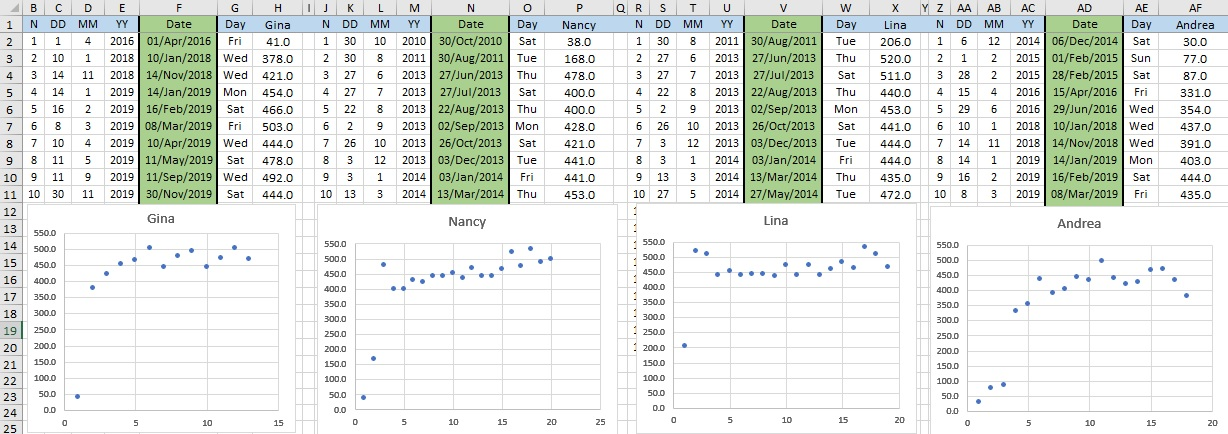
\includegraphics[scale=0.5]{img/dfinicialpeso.jpg}
	 \end{center}
	 \caption{Reorganización inicial de los datos de peso.  \label{dfpesopng}}
\end{figure}

Sin embargo, tras realizar contrastes de fechas de registros de peso con las fechas de registros de leche, se encuentra con que los registros de peso coinciden parcialmente con los registros de leche en un mismo periodo. Esto quiere decir que de los pocos datos existentes respecto al peso, estos deben ser segmentados de acuerdo con el número de parto con el que coinciden las fechas de registro de producción de leche asociadas a la lactancia de ese parto. En función de lo expresado anteriormente, se debe realizar la segmentación de los datos de peso que pertenecen a cada parto (1..6) para cada vaca perteneciente a la tabla \ref{porpartosfin} de la sección anterior.\\


\subsection{Agrupación de datos de peso}
De la tabla \ref{Nporpartos} se tienen 18 vacas diferentes para un total de 28 partos distintos que dependiendo del número de parto se cuenta con una cantidad de muestras distinta (Entre 162 y 309 muestras). Ahora bien, para los análisis algorítmicos en Matlab y/o Python, se requiere que la cantidad de muestras de leche tengan la misma cantidad de muestras para el peso en pro de lograr un análisis por ``Ecuaciones Diferenciales Ordinarias''; por tanto es necesario realizar una interpolación del(los) dato(s) de peso dependiendo de la cantidad de muestras presentes en cada parto.
%=================================================
% Please add the following required packages to your document preamble:
% \usepackage{multirow}
% \usepackage{graphicx}
% \usepackage[table,xcdraw]{xcolor}
% If you use beamer only pass "xcolor=table" option, i.e. \documentclass[xcolor=table]{beamer}
% Please add the following required packages to your document preamble:
% \usepackage{multirow}
% \usepackage{graphicx}
% \usepackage[table,xcdraw]{xcolor}
% If you use beamer only pass "xcolor=table" option, i.e. \documentclass[xcolor=table]{beamer}
\begin{table}[H]
\centering
\caption{Cantidad de muestras para cada vaca de cada parto}
\label{Nporpartos}
\resizebox{\textwidth}{!}{%
\begin{tabular}{|
>{\columncolor[HTML]{FFCE93}}c |
>{\columncolor[HTML]{C0C0C0}}c |
>{\columncolor[HTML]{A3E1F3}}c 
>{\columncolor[HTML]{A3E1F3}}c |
>{\columncolor[HTML]{A1DA8E}}c 
>{\columncolor[HTML]{A1DA8E}}c |
>{\columncolor[HTML]{FFFFC7}}c 
>{\columncolor[HTML]{FFFFC7}}c |
>{\columncolor[HTML]{F39E9E}}c |
>{\columncolor[HTML]{B791DE}}c |}
\hline
\textbf{\# de Parto} &
  \cellcolor[HTML]{343434}{\color[HTML]{FFFFFF} \textit{\textbf{1}}} &
  \multicolumn{2}{c|}{\cellcolor[HTML]{1122C6}{\color[HTML]{FFFFFF} \textit{\textbf{2}}}} &
  \multicolumn{2}{c|}{\cellcolor[HTML]{32CB00}\textit{\textbf{3}}} &
  \multicolumn{2}{c|}{\cellcolor[HTML]{FFFE65}\textit{\textbf{4}}} &
  \cellcolor[HTML]{EF3B3B}\textit{\textbf{5}} &
  \cellcolor[HTML]{AD71EB}\textit{\textbf{6}} \\ \hline
\textit{\textbf{\# de Muestras}} &
  \textbf{299} &
  \multicolumn{2}{c|}{\cellcolor[HTML]{A3E1F3}\textbf{288}} &
  \multicolumn{2}{c|}{\cellcolor[HTML]{A1DA8E}\textbf{309}} &
  \multicolumn{2}{c|}{\cellcolor[HTML]{FFFFC7}\textbf{274}} &
  \textbf{298} &
  \textbf{162} \\ \hline
\cellcolor[HTML]{FFCE93} &
  \textit{\textbf{Acerada}} &
  \multicolumn{1}{c|}{\cellcolor[HTML]{A3E1F3}\textit{\textbf{Dianita}}} &
  \textit{\textbf{Pacha}} &
  \multicolumn{1}{c|}{\cellcolor[HTML]{A1DA8E}\textit{\textbf{Fernanda}}} &
  \textit{\textbf{Martina}} &
  \multicolumn{1}{c|}{\cellcolor[HTML]{FFFFC7}\textit{\textbf{Centavito}}} &
  \textit{\textbf{Muchira}} &
  \textit{\textbf{Andrea}} &
  \textit{\textbf{Andrea}} \\ \cline{2-10} 
\cellcolor[HTML]{FFCE93} &
  \textit{\textbf{Lunita}} &
  \multicolumn{1}{c|}{\cellcolor[HTML]{A3E1F3}\textit{\textbf{Gina}}} &
  \textit{\textbf{Sol}} &
  \multicolumn{1}{c|}{\cellcolor[HTML]{A1DA8E}\textit{\textbf{Guapa}}} &
  \textit{\textbf{Morocha}} &
  \multicolumn{1}{c|}{\cellcolor[HTML]{FFFFC7}\textit{\textbf{Dianita}}} &
  \textit{\textbf{Soraya}} &
  \textit{\textbf{Guapa}} &
  \textit{\textbf{Guapa}} \\ \cline{2-10} 
\cellcolor[HTML]{FFCE93} &
  \textit{\textbf{Sol}} &
  \multicolumn{1}{c|}{\cellcolor[HTML]{A3E1F3}\textit{\textbf{Juanita}}} &
  \textit{\textbf{Viviana}} &
  \multicolumn{1}{c|}{\cellcolor[HTML]{A1DA8E}\textit{\textbf{Juanita}}} &
  \textit{\textbf{Sol}} &
  \multicolumn{1}{c|}{\cellcolor[HTML]{FFFFC7}\textit{\textbf{Leticia}}} &
  \textit{\textbf{Viviana}} &
  \textit{\textbf{}} &
  \textit{\textbf{}} \\ \cline{2-10} 
\multirow{-4}{*}{\cellcolor[HTML]{FFCE93}\textbf{\begin{tabular}[c]{@{}c@{}}Vacas \\ participantes\end{tabular}}} &
  \textit{\textbf{}} &
  \multicolumn{1}{c|}{\cellcolor[HTML]{A3E1F3}\textit{\textbf{Lucia}}} &
  \textit{\textbf{}} &
  \multicolumn{1}{c|}{\cellcolor[HTML]{A1DA8E}\textit{\textbf{Leticia}}} &
  \textit{\textbf{}} &
  \multicolumn{1}{c|}{\cellcolor[HTML]{FFFFC7}\textit{\textbf{Morocha}}} &
  \textit{\textbf{}} &
  \textit{\textbf{}} &
  \textit{\textbf{}} \\ \hline
\end{tabular}%
}
\end{table}
%=================================================

\subsubsection{Generación de columnas de peso que serán anexadas a los ``dataframes'' de cada uno de los modelos asociados al número de parto modelado}

El método usado para realizar la interpolación entre los datos de peso son las ``Splines Cúbicas'' que varían en tamaño dependiendo de la cantidad de datos presentes en cada parto. Una vez ejecutado el script de Matlab ``InterpPesosPartesEDOs'' (adjunto en este trabajo de grado)' se obtiene el conjunto de arreglos unidimensionales con los tamaños deseados (ver figura \ref{interpesospng}) y se procede a realizar la exportación correspondiente en archivos separados por comas. Posteriormente se procede a agruparlos en ``dataframes'' para su análisis por EDOs en python. Para cada lactancia se tendrá un ``dataframe'' representativo de ese modelo con las columnas de producciones de leche, peso y estiércol producido por cada vaca perteneciente a esa agrupación de lactancia.

\begin{figure}[H]
	 \begin{center}
	 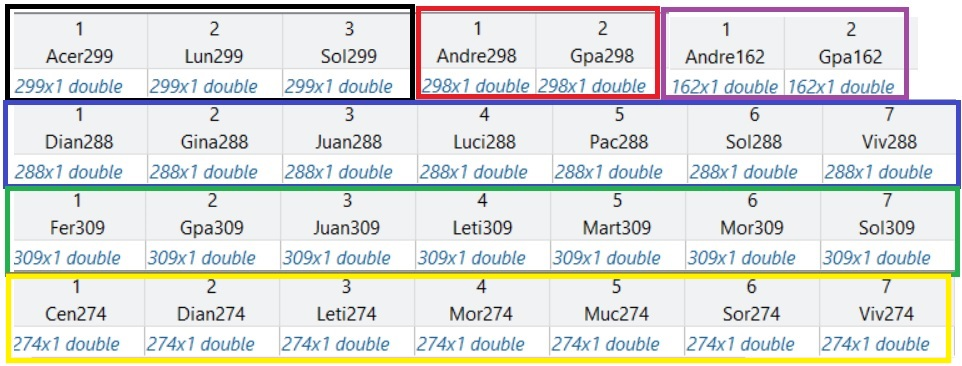
\includegraphics[scale=0.64]{img/InterPesos.jpg}
	 \end{center}
	 \caption{Formato de nombre de columna para conjunto de datos. Varia en cuanto al nombre de la vaca, cantidad de muestras existentes y cantidad de parto. El código de colores se mantiene según la tabla \ref{colorpartos} \label{interpesospng}}
\end{figure}


Llegados a este punto, ya se cuenta con los datos de las 3 variables necesarias (Producción de Leche, Estiércol, Peso) para plantear el (los) modelo(s) por EDOs, descrito en el próximo capitulo.
%================================================================================================


\chapter{CRISP - DM: ETAPA \#4 \\ Modelado}\label{crisp4}
\label{crisp4}
Al final del capítulo \ref{crisp3}, se obtienen, tanto los datos referentes a la producción de leche de cada vaca en cada parto, así como también los datos referentes al peso de las reses asociadas a dicha producción. En este capítulo se hablará del ajuste de curvas para los datos de lactancia en cada parto y del plantemiento de modelo(s) con EDOs.

\section{Ajuste de Curvas mediante funciones No lineales}\label{ajustenonlin}

A diferencia de la leche, los datos interpolados de peso pueden presentar una variabilidad  creciente al rededor de un valor de equilibrio, o por el contrario ser asumidos como valores constantes desde la última medición existente (esto es, en aquellos casos que se desconocen lo registros de peso por motivos de fuerza mayor, como por ejemplo la Pandemia del SARS CoV 2, a la que se le atribuye que muchos datos no hayan sido medidos entre el 2020 y 2022). Cualquiera que sea el caso, el peso puede ser descrito a simple vista por una curva distinguible; esto dado que son curvas interpoladas basadas en un único conjunto de datos para cada res.\\

Por su parte, la producción de leche grupal depende de la suma de las producciones de leche asociadas a cada grupo de partos; y para una representación individual los datos existentes poseen error añadido, ya sea por medición, error humano, error de aproximación, entre otros. Por tanto no es posible identificar una curva única que pueda representar a todos los datos de una forma generalizada. Para tener en consideración una curva representativa de los datos de cada parto, o una curva representativa de los datos de cada lactancia, se pueden realizar ajustes de curvas de lactancia, teniendo en consideración que ya existen modelos matemáticos probados para representar este tipo de datos. Entre estos modelos existentes, utilizaremos como referencia el modelo no lineal de Gamma Invertida de Wood, dado que según \cite{silvestre} y \cite{shanks}, es un modelo más que apropiado para aquellas curvas ``normales'' con una etapa creciente hasta el punto de producción máxima y una etapa decreciente hasta el periodo de secado.\\
 
\subsection{Método de ajuste no lineal: Levenberg-Marquardt (LM)}

El ajuste de curvas es un proceso que se utiliza para encontrar una función matemática que mejor se ajuste a un conjunto de datos experimentales. Una de las técnicas más populares para el ajuste de curvas es el método de Levenberg-Marquardt, que es una combinación de los métodos de Gauss-Newton y el método del gradiente conjugado \cite{levenberduke}. El método de LM es muy eficiente en la resolución de problemas de ajuste de curvas no lineales, y es ampliamente utilizado en diversas áreas de la ciencia y la ingeniería, incluyendo la física, la química, la biología, la economía y la ingeniería.\\

En términos generales, el método de LM minimiza la función de error cuadrático entre los datos experimentales y el modelo teórico. Este método se basa en un enfoque iterativo que comienza con una estimación inicial de los parámetros de la función de ajuste y se ajusta sucesivamente hasta que se alcanza una solución que minimiza la función de error cuadrático. El método de LM utiliza una matriz jacobiana para calcular la dirección del gradiente y la tasa de aprendizaje de cada paso iterativo. La matriz jacobiana se utiliza para calcular la dirección del gradiente y la tasa de aprendizaje de cada paso iterativo. Si la tasa de aprendizaje es grande, el método funciona como el método del gradiente conjugado. Si la tasa de aprendizaje es pequeña, el método funciona como el método de Gauss-Newton. Por lo tanto, el método de Levenberg-Marquardt es una combinación de ambos métodos \cite{levenberduke}.\\

Teniendo en consideración que el método de LM es implementado tomando como base el script público de \cite{levenberduke}, se pueden obtener unos primeros ajustes como los de la figura \ref{levenberg1}:

\begin{figure}[H]
	 \begin{center}
	 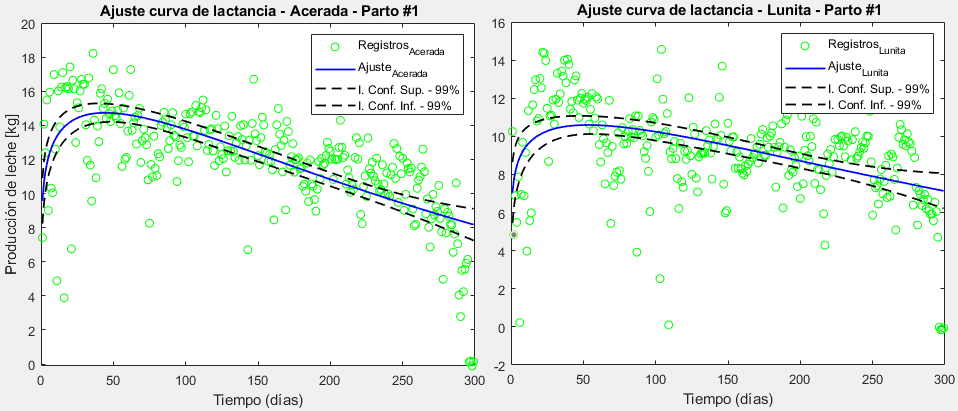
\includegraphics[scale=0.64]{img/lev1p1.png}
	 \end{center}
	 \caption{Ajustes de curvas de lactancia para Acerada y Lunita, Parto\#1.  \label{levenberg1}}
\end{figure}

De los resultados obtenidos por el método anterior, se pueden estimar los valores de los parámetros $\alpha$, $\beta$ y $\gamma$ para cada una de las reses. Teniéndose como resultado un total de 84 parámetros usados para representas las 28 curvas de lactancia para las vacas de la tabla \ref{Nporpartos}. Este algoritmo es especialmente útil para evidenciar las ejecuciones del mismo hasta lograr la aproximación de los parámetros de interés:

\begin{figure}[H]
	 \begin{center}
	 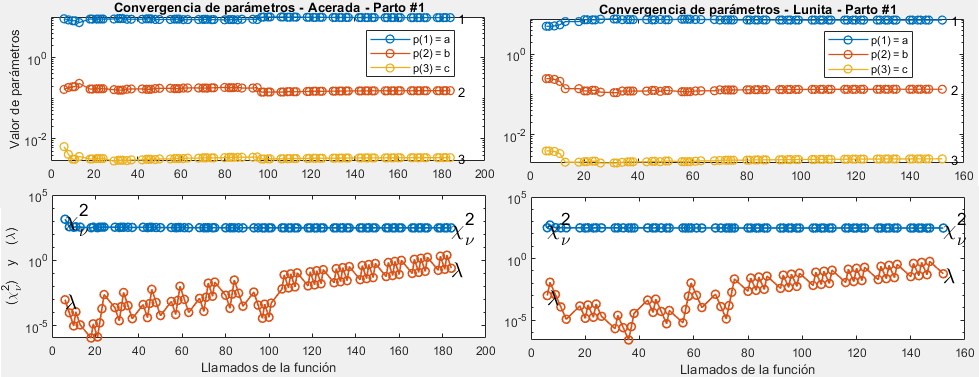
\includegraphics[scale=0.64]{img/parslev1.png}
	 \end{center}
	 \caption{Convergencia de parámetros estimados del modelo de Wood para Acerada y Lunita. \label{levenberg1}}
\end{figure}

% Feb 19 2023----- Debería tener una tabla con 84 los parámetros hallados por LM, por MIXED y por ESTOCASTICOS ?? Preguntar a Tobón

\subsection{Método de ajuste no lineal: Efectos mixtos (ME)}

Para este caso, los sujetos de estudio son las reses de cada parto y se busca estimar los parámetros de ajuste de cada vaca aún cuando el modelo plantee una solución generalizada para cada parto.


Supóngase que se realiza un ajuste no-lineal como el de Levenberg-Marquardt a las reses de cada parto, obteniéndose las figuras \ref{nlinfit1png} y \ref{nlinfitbox1png}:

\begin{figure}[H]
	 \begin{center}
	 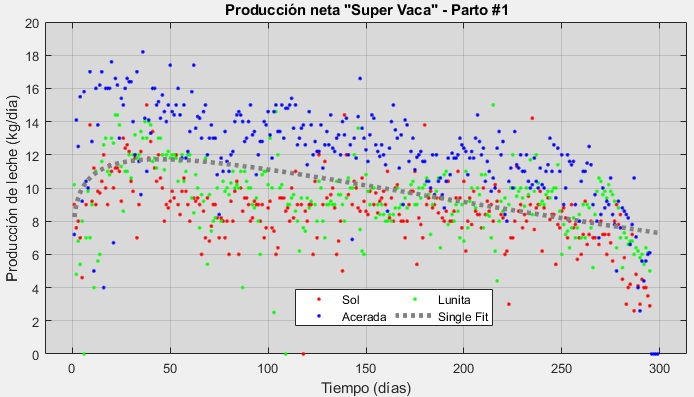
\includegraphics[scale=0.69]{img/nlinfit1spa.jpg}
	 \end{center}
	 \caption{Estimación no Lineal de parámetros generalizado del modelo de Wood para las reses del parto 1. \label{nlinfit1png}}
\end{figure}

De la figura \ref{nlinfitbox1png} se puede observar que los residuos de las reses del parto 1 se encuentran por encima o por debajo de 0, lo que indica que el modelo ha fallado en identificar los efectos específicos en el sujeto. Para lograr la identificación de los efectos específicos de cada vaca se debe hacer un ajuste individual tal y como se observa en la figura \ref{nlinfitmultiplepng}:

\begin{figure}[H]
	 \begin{center}
	 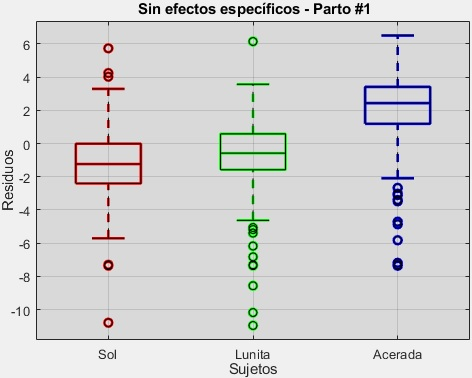
\includegraphics[scale=0.7]{img/nlinfitbox1spa.jpg}
	 \end{center}
	 \caption{Diagrama de cajas y bigotes para las reses del parto 1. \label{nlinfitbox1png}}
\end{figure}

\begin{figure}[H]
	 \begin{center}
	 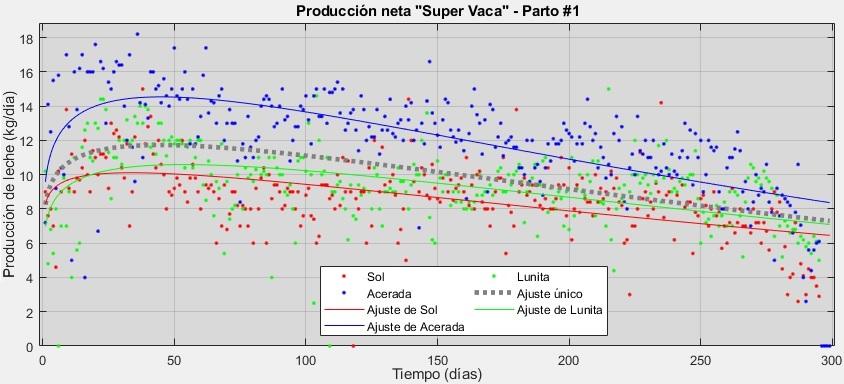
\includegraphics[scale=0.69]{img/nlinfitmultiplespa.jpg}
	 \end{center}
	 \caption{Estimación no Lineal de parámetros individualizado del modelo de Wood para las reses del parto 1. \label{nlinfitmultiplepng}}
\end{figure}

Repitiendo este proceso de comparación, se puede observar que incluso para aquellos partos que cuentan con 7 reses, la estimación individualizada permite una disminución del  error cuadrático medio concluyendo así que el ajuste para efectos específicos representa mejor ajuste que el modelo generalizado. Por otra parte, los diagramas de cajas y bigotes también muestran una mejoría notable, pues se evidencia que los residuos del ajuste tienden a estar centrados en 0, y el tamaño de las cajas disminuye a comparación del modelo anterior.

\begin{figure}[H]
	 \begin{center}
	 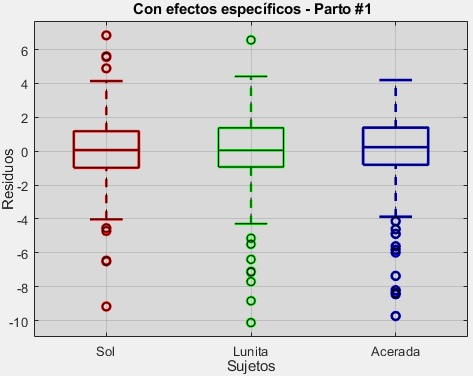
\includegraphics[scale=0.9]{img/nlinfitboxmultiplespa.jpg}
	 \end{center}
	 \caption{Diagrama de cajas y bigotes individualizado para las reses del parto 1. \label{nlinfitbox1png}}
\end{figure}

Aún cuando este ajuste ha probado tener mejores resultados que el ajuste no lineal por el método de LM, y explica con éxito las variaciones debidas a los sujetos específicos del estudio, no considera a los sujetos como representantes de una población más grande, esto es, para casos donde se tuvieran más sujetos de estudio a comparación de los existentes. El propósito de los modelos de efectos mixtos es dar cuenta de las variaciones específicas de los sujetos de manera más amplia, como efectos aleatorios que varían en torno a las medias de la población. Por tal motivo se considera pertinente realizar un análisis complementario para un ajuste no lineal con efectos mixtos aleatorios. %  mediante el uso de efectos mixtos estocásticos.
\pagebreak
% \subsection{Método de ajuste no lineal: Efectos mixtos estocásticos}
\subsection{Método de ajuste no lineal: Efectos mixtos (ME) aleatorios}

En este caso, el método de ajuste no lineal utilizado con anterioridad es cambiado por la función de ajuste no lineal de efectos mixtos ``nlmefit'', la que por defecto  asigna efectos aleatorios a todos los parámetros del modelo. También de forma predeterminada, asume una matriz sin covarianza entre los efectos aleatorios para evitar la parametrización excesiva y los problemas de convergencia relacionados.\\

De esta función, utilizada en Matlab, se pueden extraer algunos criterios adicionales que puedes complementar las decisiones tomadas en el método, como por ejemplo la reducción de los parámetros AIC y BIC. El criterio de información de Akaike (AIC) y el criterio de información bayesiano (BIC) son dos medidas de la calidad del ajuste de un modelo estadístico, que se utilizan comúnmente para seleccionar el mejor modelo entre varios modelos candidatos. En general, se prefiere un modelo con un valor más bajo de AIC o BIC, ya que esto indica que el modelo tiene una buena bondad de ajuste y una complejidad adecuada. Sin embargo, no hay un umbral fijo para considerar un modelo ``bueno'' o ``malo'' en términos de estos criterios. En cambio, se comparan los valores de AIC o BIC de varios modelos candidatos para seleccionar el mejor modelo \cite{matlabmixed}.\\

La matriz de covarianza generada para cada parto puede presentar algunos valores cercanos a 0. Este tipo de valores sugieren que los efectos aleatorios en esos parámetros pueden removerse para simplificar el modelo. Esto se logra y se justifica nuevamente al notar que los criterios AIC y BIC disminuyen nuevamente.

Para evidenciar la relación existente entre parámetros, es posible graficar las matrices de covarianza del método ``nlmefit'', en donde los valores altamente correlacionados son cercanos a 1 y los que no, son forzados a 0. Para este trabajo de grado, se obtienen las relaciones en las matrices de covarianza mostradas en la figura  \ref{covmatricespng}. Identifíquese que el modelo de Wood requiere de la estimación de 3 parámetros por lo que originalmente las matrices de correlación entre parámetros aleatorios deberían ser de dimensión 3 para todos los partos, pero como algunas correlaciones a aleatorios resultan ser cercanas a 0, esta dimensión disminuye en algunos casos, ocasionando que la complejidad de ajuste sea mucho menor. Nuevamente estos resultados son soportados por la disminución en los criterios AIC y BIC, que aunque la disminución no es considerable, es menor a la anterior y por tanto representa un mejor ajuste.\\

Finalmente, una vez ejecuta el método nuevamente y teniendo en cuenta las consideraciones mencionadas hasta este momento, se generan los parámetros $b_{i}$, encargados de entregar las predicciones de los parámetros para cada una de las reses; con lo que se procede a sumar $b_{i}$ con los estimados de efectos fijos para producir el modelo de efectos mixtos final. Este proceso se repite para cada uno de los partos mediante un bucle, pero por motivos de espacio y lectura no son mostrados a continuación. (Ver script de Matlab denominado ``AnaMixEffGenBeta.m''). Los resultados obtenidos por el modelo de efectos mixtos son contrastados con la primer estimación no lineal del método de LM y mostrados en la figura \ref{mixedfinalpng}:

\begin{figure}[H]
	 \begin{center}
	 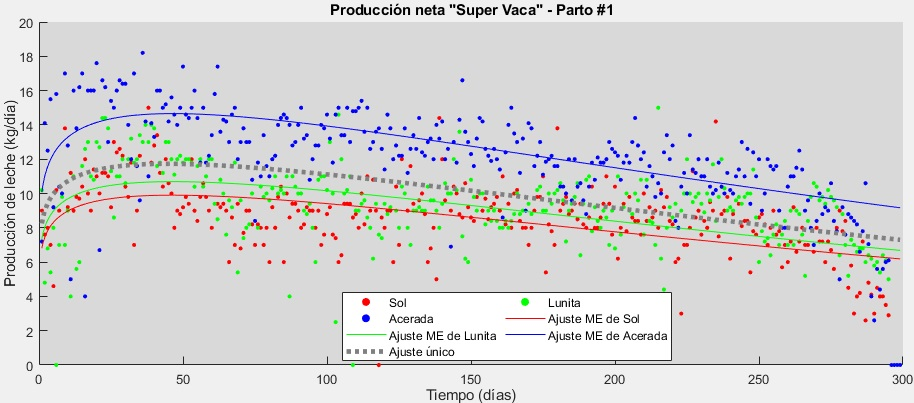
\includegraphics[scale=0.60]{img/mixedfinalspa.jpg}
	 \end{center}
	 \caption{Comparación final entre: a) Ajuste por efectos mixtos y b) Ajuste no-lineal por LM . \label{mixedfinalpng}}
\end{figure}

Adicionalmente, si no tenemos en cuenta la poca cantidad de valores atípicos existentes en los datos y evidenciados en los diagramas de cajas y bigotes; se puede establecer que la siguiente gráfica de probabilidad normal de los residuos muestra un acuerdo razonable con los supuestos del modelo sobre los errores (ver figura \ref{residprobnormpng})

\begin{figure}[H]
	 \begin{center}
	 \includegraphics[scale=0.7]{img/residprobnormspa.jpg}
	 \end{center}
	 \caption{Gráfica de probabilidad normal en los residuos. Parto \#1. \label{residprobnormpng}}
\end{figure}

Cabe resaltar que este análisis es llevado a cabo para cada res y cada parto, pero por motivos de espacio y extensión de este trabajo; solo se muestran resultados del primer parto. Las demás gráficas y valores pueden ser corroborados en los scripts de Matlab y Python.

\begin{figure}[H]
	 \begin{center}
	 \includegraphics[scale=0.64]{img/covmatricesspa.jpg}
	 \end{center}
	 \caption{Correlación de parámetros por efectos aleatorios. \label{covmatricespng}}
\end{figure}

\pagebreak

% Please add the following required packages to your document preamble:
% \usepackage{multirow}
% \usepackage{graphicx}
% \usepackage[table,xcdraw]{xcolor}
% If you use beamer only pass "xcolor=table" option, i.e. \documentclass[xcolor=table]{beamer}
% Please add the following required packages to your document preamble:
% \usepackage{multirow}
% \usepackage{graphicx}
% \usepackage[table,xcdraw]{xcolor}
% If you use beamer only pass "xcolor=table" option, i.e. \documentclass[xcolor=table]{beamer}

% \begin{table}[]
% \centering
% \caption{Resumen de los parámetros de ajuste para cada método usado.}
% \label{tab:allparams}
% \resizebox{\textwidth}{!}{%
% \begin{tabular}{|ccc|cccccccccccccccccc|}
% \hline
% \rowcolor[HTML]{FFD9AC} 
% \multicolumn{3}{|c|}{\cellcolor[HTML]{FFD9AC}} &
%   \multicolumn{3}{c|}{\cellcolor[HTML]{FFD9AC}\textbf{EMPÍRICOS}} &
%   \multicolumn{3}{c|}{\cellcolor[HTML]{FFD9AC}\textbf{"FIT" - LM}} &
%   \multicolumn{3}{c|}{\cellcolor[HTML]{FFD9AC}\textbf{"FIT" - UNICO}} &
%   \multicolumn{3}{c|}{\cellcolor[HTML]{FFD9AC}\textbf{"FIT" - EM F}} &
%   \multicolumn{3}{c|}{\cellcolor[HTML]{FFD9AC}\textbf{"FIT" - EM A}} &
%   \multicolumn{3}{c|}{\cellcolor[HTML]{FFD9AC}\textbf{PROM}} \\ \hline
% \rowcolor[HTML]{FFD9AC} 
% \multicolumn{1}{|c|}{\cellcolor[HTML]{FFD9AC}} &
%   \multicolumn{1}{c|}{\cellcolor[HTML]{FFD9AC}} &
%   \textbf{PARS} &
%   \multicolumn{1}{c|}{\cellcolor[HTML]{FFD9AC}\textbf{a}} &
%   \multicolumn{1}{c|}{\cellcolor[HTML]{FFD9AC}\textbf{b}} &
%   \multicolumn{1}{c|}{\cellcolor[HTML]{FFD9AC}\textbf{c}} &
%   \multicolumn{1}{c|}{\cellcolor[HTML]{FFD9AC}\textbf{a}} &
%   \multicolumn{1}{c|}{\cellcolor[HTML]{FFD9AC}\textbf{b}} &
%   \multicolumn{1}{c|}{\cellcolor[HTML]{FFD9AC}\textbf{c}} &
%   \multicolumn{1}{c|}{\cellcolor[HTML]{FFD9AC}\textbf{a}} &
%   \multicolumn{1}{c|}{\cellcolor[HTML]{FFD9AC}\textbf{b}} &
%   \multicolumn{1}{c|}{\cellcolor[HTML]{FFD9AC}\textbf{c}} &
%   \multicolumn{1}{c|}{\cellcolor[HTML]{FFD9AC}\textbf{a}} &
%   \multicolumn{1}{c|}{\cellcolor[HTML]{FFD9AC}\textbf{b}} &
%   \multicolumn{1}{c|}{\cellcolor[HTML]{FFD9AC}\textbf{c}} &
%   \multicolumn{1}{c|}{\cellcolor[HTML]{FFD9AC}\textbf{a}} &
%   \multicolumn{1}{c|}{\cellcolor[HTML]{FFD9AC}\textbf{b}} &
%   \multicolumn{1}{c|}{\cellcolor[HTML]{FFD9AC}\textbf{c}} &
%   \multicolumn{1}{c|}{\cellcolor[HTML]{FFD9AC}\textbf{a}} &
%   \multicolumn{1}{c|}{\cellcolor[HTML]{FFD9AC}\textbf{b}} &
%   \textbf{c} \\ \cline{3-21} 
% \rowcolor[HTML]{FFD9AC} 
% \multicolumn{1}{|c|}{\multirow{-2}{*}{\cellcolor[HTML]{FFD9AC}\textbf{\begin{tabular}[c]{@{}c@{}}PARTO\\   P \#i\end{tabular}}}} &
%   \multicolumn{1}{c|}{\multirow{-2}{*}{\cellcolor[HTML]{FFD9AC}\textbf{N}}} &
%   \textbf{VACA} &
%   \multicolumn{18}{c|}{\cellcolor[HTML]{FFD9AC}} \\ \hline
% \multicolumn{1}{|c|}{\cellcolor[HTML]{343434}{\color[HTML]{FFFFFF} }} &
%   \multicolumn{1}{c|}{\cellcolor[HTML]{343434}{\color[HTML]{FFFFFF} }} &
%   \cellcolor[HTML]{656565}{\color[HTML]{FFFFFF} \textbf{ACER}} &
%   \multicolumn{1}{c|}{\textit{\textbf{15.500}}} &
%   \multicolumn{1}{c|}{\textit{\textbf{0.045}}} &
%   \multicolumn{1}{c|}{\textit{\textbf{0.007}}} &
%   \multicolumn{1}{c|}{\textit{\textbf{9.602}}} &
%   \multicolumn{1}{c|}{\textit{\textbf{0.153}}} &
%   \multicolumn{1}{c|}{\textit{\textbf{0.004}}} &
%   \multicolumn{1}{c|}{} &
%   \multicolumn{1}{c|}{} &
%   \multicolumn{1}{c|}{} &
%   \multicolumn{1}{c|}{\textit{\textbf{9.612}}} &
%   \multicolumn{1}{c|}{\textit{\textbf{0.147}}} &
%   \multicolumn{1}{c|}{\textit{\textbf{0.003}}} &
%   \multicolumn{1}{c|}{\textit{\textbf{10.098}}} &
%   \multicolumn{1}{c|}{\textit{\textbf{0.131}}} &
%   \multicolumn{1}{c|}{\textit{\textbf{0.003}}} &
%   \multicolumn{1}{c|}{\textit{\textbf{10.617}}} &
%   \multicolumn{1}{c|}{\textit{\textbf{0.120}}} &
%   \textit{\textbf{0.004}} \\ \cline{3-9} \cline{13-21} 
% \multicolumn{1}{|c|}{\cellcolor[HTML]{343434}{\color[HTML]{FFFFFF} }} &
%   \multicolumn{1}{c|}{\cellcolor[HTML]{343434}{\color[HTML]{FFFFFF} }} &
%   \cellcolor[HTML]{656565}{\color[HTML]{FFFFFF} \textbf{SOL}} &
%   \multicolumn{1}{c|}{\textit{\textbf{7.000}}} &
%   \multicolumn{1}{c|}{\textit{\textbf{0.210}}} &
%   \multicolumn{1}{c|}{\textit{\textbf{0.008}}} &
%   \multicolumn{1}{c|}{\textit{\textbf{7.405}}} &
%   \multicolumn{1}{c|}{\textit{\textbf{0.119}}} &
%   \multicolumn{1}{c|}{\textit{\textbf{0.003}}} &
%   \multicolumn{1}{c|}{} &
%   \multicolumn{1}{c|}{} &
%   \multicolumn{1}{c|}{} &
%   \multicolumn{1}{c|}{\textit{\textbf{8.295}}} &
%   \multicolumn{1}{c|}{\textit{\textbf{0.079}}} &
%   \multicolumn{1}{c|}{\textit{\textbf{0.002}}} &
%   \multicolumn{1}{c|}{\textit{\textbf{6.833}}} &
%   \multicolumn{1}{c|}{\textit{\textbf{0.131}}} &
%   \multicolumn{1}{c|}{\textit{\textbf{0.003}}} &
%   \multicolumn{1}{c|}{\textit{\textbf{7.561}}} &
%   \multicolumn{1}{c|}{\textit{\textbf{0.133}}} &
%   \textit{\textbf{0.004}} \\ \cline{3-9} \cline{13-21} 
% \multicolumn{1}{|c|}{\multirow{-3}{*}{\cellcolor[HTML]{343434}{\color[HTML]{FFFFFF} \textbf{P \#1}}}} &
%   \multicolumn{1}{c|}{\multirow{-3}{*}{\cellcolor[HTML]{343434}{\color[HTML]{FFFFFF} \textbf{299}}}} &
%   \cellcolor[HTML]{656565}{\color[HTML]{FFFFFF} \textbf{LUN}} &
%   \multicolumn{1}{c|}{\textit{\textbf{5.400}}} &
%   \multicolumn{1}{c|}{\textit{\textbf{0.317}}} &
%   \multicolumn{1}{c|}{\textit{\textbf{0.006}}} &
%   \multicolumn{1}{c|}{\textit{\textbf{7.067}}} &
%   \multicolumn{1}{c|}{\textit{\textbf{0.136}}} &
%   \multicolumn{1}{c|}{\textit{\textbf{0.003}}} &
%   \multicolumn{1}{c|}{\multirow{-3}{*}{\textit{\textbf{8.273}}}} &
%   \multicolumn{1}{c|}{\multirow{-3}{*}{\textit{\textbf{0.125}}}} &
%   \multicolumn{1}{c|}{\multirow{-3}{*}{\textit{\textbf{0.003}}}} &
%   \multicolumn{1}{c|}{\textit{\textbf{6.986}}} &
%   \multicolumn{1}{c|}{\textit{\textbf{0.140}}} &
%   \multicolumn{1}{c|}{\textit{\textbf{0.003}}} &
%   \multicolumn{1}{c|}{\textit{\textbf{7.375}}} &
%   \multicolumn{1}{c|}{\textit{\textbf{0.131}}} &
%   \multicolumn{1}{c|}{\textit{\textbf{0.003}}} &
%   \multicolumn{1}{c|}{\textit{\textbf{7.020}}} &
%   \multicolumn{1}{c|}{\textit{\textbf{0.170}}} &
%   \textit{\textbf{0.003}} \\ \hline
% \multicolumn{1}{|c|}{\cellcolor[HTML]{3241CB}{\color[HTML]{FFFFFF} }} &
%   \multicolumn{1}{c|}{\cellcolor[HTML]{3241CB}{\color[HTML]{FFFFFF} }} &
%   \cellcolor[HTML]{BDFFFC}\textbf{DIAN} &
%   \multicolumn{1}{c|}{\textit{\textbf{21.000}}} &
%   \multicolumn{1}{c|}{\textit{\textbf{0.080}}} &
%   \multicolumn{1}{c|}{\textit{\textbf{0.005}}} &
%   \multicolumn{1}{c|}{\textit{\textbf{15.930}}} &
%   \multicolumn{1}{c|}{\textit{\textbf{0.114}}} &
%   \multicolumn{1}{c|}{\textit{\textbf{0.004}}} &
%   \multicolumn{1}{c|}{} &
%   \multicolumn{1}{c|}{} &
%   \multicolumn{1}{c|}{} &
%   \multicolumn{1}{c|}{\textit{\textbf{16.220}}} &
%   \multicolumn{1}{c|}{\textit{\textbf{0.107}}} &
%   \multicolumn{1}{c|}{\textit{\textbf{0.004}}} &
%   \multicolumn{1}{c|}{\textit{\textbf{16.154}}} &
%   \multicolumn{1}{c|}{\textit{\textbf{0.109}}} &
%   \multicolumn{1}{c|}{\textit{\textbf{0.004}}} &
%   \multicolumn{1}{c|}{\textit{\textbf{16.303}}} &
%   \multicolumn{1}{c|}{\textit{\textbf{0.113}}} &
%   \textit{\textbf{0.014}} \\ \cline{3-9} \cline{13-21} 
% \multicolumn{1}{|c|}{\cellcolor[HTML]{3241CB}{\color[HTML]{FFFFFF} }} &
%   \multicolumn{1}{c|}{\cellcolor[HTML]{3241CB}{\color[HTML]{FFFFFF} }} &
%   \cellcolor[HTML]{BDFFFC}\textbf{GINA} &
%   \multicolumn{1}{c|}{\textit{\textbf{20.400}}} &
%   \multicolumn{1}{c|}{\textit{\textbf{0.168}}} &
%   \multicolumn{1}{c|}{\textit{\textbf{0.009}}} &
%   \multicolumn{1}{c|}{\textit{\textbf{11.950}}} &
%   \multicolumn{1}{c|}{\textit{\textbf{0.251}}} &
%   \multicolumn{1}{c|}{\textit{\textbf{0.007}}} &
%   \multicolumn{1}{c|}{} &
%   \multicolumn{1}{c|}{} &
%   \multicolumn{1}{c|}{} &
%   \multicolumn{1}{c|}{\textit{\textbf{16.059}}} &
%   \multicolumn{1}{c|}{\textit{\textbf{0.149}}} &
%   \multicolumn{1}{c|}{\textit{\textbf{0.006}}} &
%   \multicolumn{1}{c|}{\textit{\textbf{15.553}}} &
%   \multicolumn{1}{c|}{\textit{\textbf{0.158}}} &
%   \multicolumn{1}{c|}{\textit{\textbf{0.006}}} &
%   \multicolumn{1}{c|}{\textit{\textbf{15.234}}} &
%   \multicolumn{1}{c|}{\textit{\textbf{0.176}}} &
%   \textit{\textbf{0.016}} \\ \cline{3-9} \cline{13-21} 
% \multicolumn{1}{|c|}{\cellcolor[HTML]{3241CB}{\color[HTML]{FFFFFF} }} &
%   \multicolumn{1}{c|}{\cellcolor[HTML]{3241CB}{\color[HTML]{FFFFFF} }} &
%   \cellcolor[HTML]{BDFFFC}\textbf{JUAN} &
%   \multicolumn{1}{c|}{\textit{\textbf{9.400}}} &
%   \multicolumn{1}{c|}{\textit{\textbf{0.126}}} &
%   \multicolumn{1}{c|}{\textit{\textbf{0.010}}} &
%   \multicolumn{1}{c|}{\textit{\textbf{4.103}}} &
%   \multicolumn{1}{c|}{\textit{\textbf{0.317}}} &
%   \multicolumn{1}{c|}{\textit{\textbf{0.008}}} &
%   \multicolumn{1}{c|}{} &
%   \multicolumn{1}{c|}{} &
%   \multicolumn{1}{c|}{} &
%   \multicolumn{1}{c|}{\textit{\textbf{4.384}}} &
%   \multicolumn{1}{c|}{\textit{\textbf{0.282}}} &
%   \multicolumn{1}{c|}{\textit{\textbf{0.007}}} &
%   \multicolumn{1}{c|}{\textit{\textbf{5.119}}} &
%   \multicolumn{1}{c|}{\textit{\textbf{0.233}}} &
%   \multicolumn{1}{c|}{\textit{\textbf{0.007}}} &
%   \multicolumn{1}{c|}{\textit{\textbf{7.043}}} &
%   \multicolumn{1}{c|}{\textit{\textbf{0.222}}} &
%   \textit{\textbf{0.017}} \\ \cline{3-9} \cline{13-21} 
% \multicolumn{1}{|c|}{\cellcolor[HTML]{3241CB}{\color[HTML]{FFFFFF} }} &
%   \multicolumn{1}{c|}{\cellcolor[HTML]{3241CB}{\color[HTML]{FFFFFF} }} &
%   \cellcolor[HTML]{BDFFFC}\textbf{LUCI} &
%   \multicolumn{1}{c|}{\textit{\textbf{19.000}}} &
%   \multicolumn{1}{c|}{\textit{\textbf{0.028}}} &
%   \multicolumn{1}{c|}{\textit{\textbf{0.005}}} &
%   \multicolumn{1}{c|}{\textit{\textbf{13.394}}} &
%   \multicolumn{1}{c|}{\textit{\textbf{0.167}}} &
%   \multicolumn{1}{c|}{\textit{\textbf{0.007}}} &
%   \multicolumn{1}{c|}{} &
%   \multicolumn{1}{c|}{} &
%   \multicolumn{1}{c|}{} &
%   \multicolumn{1}{c|}{\textit{\textbf{13.801}}} &
%   \multicolumn{1}{c|}{\textit{\textbf{0.147}}} &
%   \multicolumn{1}{c|}{\textit{\textbf{0.006}}} &
%   \multicolumn{1}{c|}{\textit{\textbf{13.127}}} &
%   \multicolumn{1}{c|}{\textit{\textbf{0.160}}} &
%   \multicolumn{1}{c|}{\textit{\textbf{0.006}}} &
%   \multicolumn{1}{c|}{\textit{\textbf{14.306}}} &
%   \multicolumn{1}{c|}{\textit{\textbf{0.131}}} &
%   \textit{\textbf{0.015}} \\ \cline{3-9} \cline{13-21} 
% \multicolumn{1}{|c|}{\cellcolor[HTML]{3241CB}{\color[HTML]{FFFFFF} }} &
%   \multicolumn{1}{c|}{\cellcolor[HTML]{3241CB}{\color[HTML]{FFFFFF} }} &
%   \cellcolor[HTML]{BDFFFC}\textbf{PAC} &
%   \multicolumn{1}{c|}{\textit{\textbf{18.600}}} &
%   \multicolumn{1}{c|}{\textit{\textbf{0.069}}} &
%   \multicolumn{1}{c|}{\textit{\textbf{0.004}}} &
%   \multicolumn{1}{c|}{\textit{\textbf{20.167}}} &
%   \multicolumn{1}{c|}{\textit{\textbf{-0.036}}} &
%   \multicolumn{1}{c|}{\textit{\textbf{0.002}}} &
%   \multicolumn{1}{c|}{} &
%   \multicolumn{1}{c|}{} &
%   \multicolumn{1}{c|}{} &
%   \multicolumn{1}{c|}{\textit{\textbf{19.752}}} &
%   \multicolumn{1}{c|}{\textit{\textbf{-0.027}}} &
%   \multicolumn{1}{c|}{\textit{\textbf{0.002}}} &
%   \multicolumn{1}{c|}{\textit{\textbf{18.765}}} &
%   \multicolumn{1}{c|}{\textit{\textbf{-0.010}}} &
%   \multicolumn{1}{c|}{\textit{\textbf{0.002}}} &
%   \multicolumn{1}{c|}{\textit{\textbf{17.899}}} &
%   \multicolumn{1}{c|}{\textit{\textbf{0.030}}} &
%   \textit{\textbf{0.013}} \\ \cline{3-9} \cline{13-21} 
% \multicolumn{1}{|c|}{\cellcolor[HTML]{3241CB}{\color[HTML]{FFFFFF} }} &
%   \multicolumn{1}{c|}{\cellcolor[HTML]{3241CB}{\color[HTML]{FFFFFF} }} &
%   \cellcolor[HTML]{BDFFFC}\textbf{SOL} &
%   \multicolumn{1}{c|}{\textit{\textbf{16.800}}} &
%   \multicolumn{1}{c|}{\textit{\textbf{0.078}}} &
%   \multicolumn{1}{c|}{\textit{\textbf{0.008}}} &
%   \multicolumn{1}{c|}{\textit{\textbf{10.138}}} &
%   \multicolumn{1}{c|}{\textit{\textbf{0.220}}} &
%   \multicolumn{1}{c|}{\textit{\textbf{0.007}}} &
%   \multicolumn{1}{c|}{} &
%   \multicolumn{1}{c|}{} &
%   \multicolumn{1}{c|}{} &
%   \multicolumn{1}{c|}{\textit{\textbf{9.374}}} &
%   \multicolumn{1}{c|}{\textit{\textbf{0.238}}} &
%   \multicolumn{1}{c|}{\textit{\textbf{0.007}}} &
%   \multicolumn{1}{c|}{\textit{\textbf{9.673}}} &
%   \multicolumn{1}{c|}{\textit{\textbf{0.227}}} &
%   \multicolumn{1}{c|}{\textit{\textbf{0.007}}} &
%   \multicolumn{1}{c|}{\textit{\textbf{11.639}}} &
%   \multicolumn{1}{c|}{\textit{\textbf{0.184}}} &
%   \textit{\textbf{0.016}} \\ \cline{3-9} \cline{13-21} 
% \multicolumn{1}{|c|}{\multirow{-7}{*}{\cellcolor[HTML]{3241CB}{\color[HTML]{FFFFFF} \textbf{P \#2}}}} &
%   \multicolumn{1}{c|}{\multirow{-7}{*}{\cellcolor[HTML]{3241CB}{\color[HTML]{FFFFFF} \textbf{288}}}} &
%   \cellcolor[HTML]{BDFFFC}\textbf{VIV} &
%   \multicolumn{1}{c|}{\textit{\textbf{15.400}}} &
%   \multicolumn{1}{c|}{\textit{\textbf{0.094}}} &
%   \multicolumn{1}{c|}{\textit{\textbf{0.008}}} &
%   \multicolumn{1}{c|}{\textit{\textbf{6.794}}} &
%   \multicolumn{1}{c|}{\textit{\textbf{0.339}}} &
%   \multicolumn{1}{c|}{\textit{\textbf{0.007}}} &
%   \multicolumn{1}{c|}{\multirow{-7}{*}{\textit{\textbf{12.210}}}} &
%   \multicolumn{1}{c|}{\multirow{-7}{*}{\textit{\textbf{0.154}}}} &
%   \multicolumn{1}{c|}{\multirow{-7}{*}{\textit{\textbf{0.053}}}} &
%   \multicolumn{1}{c|}{\textit{\textbf{7.847}}} &
%   \multicolumn{1}{c|}{\textit{\textbf{0.290}}} &
%   \multicolumn{1}{c|}{\textit{\textbf{0.007}}} &
%   \multicolumn{1}{c|}{\textit{\textbf{8.830}}} &
%   \multicolumn{1}{c|}{\textit{\textbf{0.256}}} &
%   \multicolumn{1}{c|}{\textit{\textbf{0.006}}} &
%   \multicolumn{1}{c|}{\textit{\textbf{10.216}}} &
%   \multicolumn{1}{c|}{\textit{\textbf{0.226}}} &
%   \textit{\textbf{0.016}} \\ \hline
% \multicolumn{1}{|c|}{\cellcolor[HTML]{32CB00}} &
%   \multicolumn{1}{c|}{\cellcolor[HTML]{32CB00}} &
%   \cellcolor[HTML]{AAFF85}\textbf{FER} &
%   \multicolumn{1}{c|}{\textit{\textbf{21.000}}} &
%   \multicolumn{1}{c|}{\textit{\textbf{0.101}}} &
%   \multicolumn{1}{c|}{\textit{\textbf{0.006}}} &
%   \multicolumn{1}{c|}{\textit{\textbf{19.729}}} &
%   \multicolumn{1}{c|}{\textit{\textbf{0.064}}} &
%   \multicolumn{1}{c|}{\textit{\textbf{0.003}}} &
%   \multicolumn{1}{c|}{} &
%   \multicolumn{1}{c|}{} &
%   \multicolumn{1}{c|}{} &
%   \multicolumn{1}{c|}{\textit{\textbf{20.217}}} &
%   \multicolumn{1}{c|}{\textit{\textbf{0.052}}} &
%   \multicolumn{1}{c|}{\textit{\textbf{0.003}}} &
%   \multicolumn{1}{c|}{\textit{\textbf{19.466}}} &
%   \multicolumn{1}{c|}{\textit{\textbf{0.067}}} &
%   \multicolumn{1}{c|}{\textit{\textbf{0.003}}} &
%   \multicolumn{1}{c|}{\textit{\textbf{18.825}}} &
%   \multicolumn{1}{c|}{\textit{\textbf{0.086}}} &
%   \textit{\textbf{0.004}} \\ \cline{3-9} \cline{13-21} 
% \multicolumn{1}{|c|}{\cellcolor[HTML]{32CB00}} &
%   \multicolumn{1}{c|}{\cellcolor[HTML]{32CB00}} &
%   \cellcolor[HTML]{AAFF85}\textbf{GPA} &
%   \multicolumn{1}{c|}{\textit{\textbf{22.000}}} &
%   \multicolumn{1}{c|}{\textit{\textbf{0.099}}} &
%   \multicolumn{1}{c|}{\textit{\textbf{0.005}}} &
%   \multicolumn{1}{c|}{\textit{\textbf{15.206}}} &
%   \multicolumn{1}{c|}{\textit{\textbf{0.148}}} &
%   \multicolumn{1}{c|}{\textit{\textbf{0.004}}} &
%   \multicolumn{1}{c|}{} &
%   \multicolumn{1}{c|}{} &
%   \multicolumn{1}{c|}{} &
%   \multicolumn{1}{c|}{\textit{\textbf{15.638}}} &
%   \multicolumn{1}{c|}{\textit{\textbf{0.132}}} &
%   \multicolumn{1}{c|}{\textit{\textbf{0.004}}} &
%   \multicolumn{1}{c|}{\textit{\textbf{15.506}}} &
%   \multicolumn{1}{c|}{\textit{\textbf{0.136}}} &
%   \multicolumn{1}{c|}{\textit{\textbf{0.004}}} &
%   \multicolumn{1}{c|}{\textit{\textbf{16.412}}} &
%   \multicolumn{1}{c|}{\textit{\textbf{0.132}}} &
%   \textit{\textbf{0.004}} \\ \cline{3-9} \cline{13-21} 
% \multicolumn{1}{|c|}{\cellcolor[HTML]{32CB00}} &
%   \multicolumn{1}{c|}{\cellcolor[HTML]{32CB00}} &
%   \cellcolor[HTML]{AAFF85}\textbf{JUAN} &
%   \multicolumn{1}{c|}{\textit{\textbf{11.000}}} &
%   \multicolumn{1}{c|}{\textit{\textbf{0.208}}} &
%   \multicolumn{1}{c|}{\textit{\textbf{0.007}}} &
%   \multicolumn{1}{c|}{\textit{\textbf{9.445}}} &
%   \multicolumn{1}{c|}{\textit{\textbf{0.203}}} &
%   \multicolumn{1}{c|}{\textit{\textbf{0.004}}} &
%   \multicolumn{1}{c|}{} &
%   \multicolumn{1}{c|}{} &
%   \multicolumn{1}{c|}{} &
%   \multicolumn{1}{c|}{\textit{\textbf{9.485}}} &
%   \multicolumn{1}{c|}{\textit{\textbf{0.202}}} &
%   \multicolumn{1}{c|}{\textit{\textbf{0.004}}} &
%   \multicolumn{1}{c|}{\textit{\textbf{9.907}}} &
%   \multicolumn{1}{c|}{\textit{\textbf{0.190}}} &
%   \multicolumn{1}{c|}{\textit{\textbf{0.004}}} &
%   \multicolumn{1}{c|}{\textit{\textbf{10.710}}} &
%   \multicolumn{1}{c|}{\textit{\textbf{0.190}}} &
%   \textit{\textbf{0.005}} \\ \cline{3-9} \cline{13-21} 
% \multicolumn{1}{|c|}{\cellcolor[HTML]{32CB00}} &
%   \multicolumn{1}{c|}{\cellcolor[HTML]{32CB00}} &
%   \cellcolor[HTML]{AAFF85}\textbf{LETI} &
%   \multicolumn{1}{c|}{\textit{\textbf{16.200}}} &
%   \multicolumn{1}{c|}{\textit{\textbf{0.116}}} &
%   \multicolumn{1}{c|}{\textit{\textbf{0.008}}} &
%   \multicolumn{1}{c|}{\textit{\textbf{15.388}}} &
%   \multicolumn{1}{c|}{\textit{\textbf{0.098}}} &
%   \multicolumn{1}{c|}{\textit{\textbf{0.004}}} &
%   \multicolumn{1}{c|}{} &
%   \multicolumn{1}{c|}{} &
%   \multicolumn{1}{c|}{} &
%   \multicolumn{1}{c|}{\textit{\textbf{16.645}}} &
%   \multicolumn{1}{c|}{\textit{\textbf{0.069}}} &
%   \multicolumn{1}{c|}{\textit{\textbf{0.003}}} &
%   \multicolumn{1}{c|}{\textit{\textbf{16.298}}} &
%   \multicolumn{1}{c|}{\textit{\textbf{0.073}}} &
%   \multicolumn{1}{c|}{\textit{\textbf{0.004}}} &
%   \multicolumn{1}{c|}{\textit{\textbf{15.648}}} &
%   \multicolumn{1}{c|}{\textit{\textbf{0.100}}} &
%   \textit{\textbf{0.005}} \\ \cline{3-9} \cline{13-21} 
% \multicolumn{1}{|c|}{\cellcolor[HTML]{32CB00}} &
%   \multicolumn{1}{c|}{\cellcolor[HTML]{32CB00}} &
%   \cellcolor[HTML]{AAFF85}\textbf{MART} &
%   \multicolumn{1}{c|}{\textit{\textbf{10.800}}} &
%   \multicolumn{1}{c|}{\textit{\textbf{0.283}}} &
%   \multicolumn{1}{c|}{\textit{\textbf{0.007}}} &
%   \multicolumn{1}{c|}{\textit{\textbf{6.613}}} &
%   \multicolumn{1}{c|}{\textit{\textbf{0.392}}} &
%   \multicolumn{1}{c|}{\textit{\textbf{0.006}}} &
%   \multicolumn{1}{c|}{} &
%   \multicolumn{1}{c|}{} &
%   \multicolumn{1}{c|}{} &
%   \multicolumn{1}{c|}{\textit{\textbf{6.516}}} &
%   \multicolumn{1}{c|}{\textit{\textbf{0.396}}} &
%   \multicolumn{1}{c|}{\textit{\textbf{0.006}}} &
%   \multicolumn{1}{c|}{\textit{\textbf{7.084}}} &
%   \multicolumn{1}{c|}{\textit{\textbf{0.371}}} &
%   \multicolumn{1}{c|}{\textit{\textbf{0.006}}} &
%   \multicolumn{1}{c|}{\textit{\textbf{8.945}}} &
%   \multicolumn{1}{c|}{\textit{\textbf{0.318}}} &
%   \textit{\textbf{0.006}} \\ \cline{3-9} \cline{13-21} 
% \multicolumn{1}{|c|}{\cellcolor[HTML]{32CB00}} &
%   \multicolumn{1}{c|}{\cellcolor[HTML]{32CB00}} &
%   \cellcolor[HTML]{AAFF85}\textbf{MOR} &
%   \multicolumn{1}{c|}{\textit{\textbf{22.000}}} &
%   \multicolumn{1}{c|}{\textit{\textbf{0.157}}} &
%   \multicolumn{1}{c|}{\textit{\textbf{0.009}}} &
%   \multicolumn{1}{c|}{\textit{\textbf{19.921}}} &
%   \multicolumn{1}{c|}{\textit{\textbf{0.108}}} &
%   \multicolumn{1}{c|}{\textit{\textbf{0.004}}} &
%   \multicolumn{1}{c|}{} &
%   \multicolumn{1}{c|}{} &
%   \multicolumn{1}{c|}{} &
%   \multicolumn{1}{c|}{\textit{\textbf{20.858}}} &
%   \multicolumn{1}{c|}{\textit{\textbf{0.092}}} &
%   \multicolumn{1}{c|}{\textit{\textbf{0.004}}} &
%   \multicolumn{1}{c|}{\textit{\textbf{20.353}}} &
%   \multicolumn{1}{c|}{\textit{\textbf{0.096}}} &
%   \multicolumn{1}{c|}{\textit{\textbf{0.004}}} &
%   \multicolumn{1}{c|}{\textit{\textbf{19.369}}} &
%   \multicolumn{1}{c|}{\textit{\textbf{0.120}}} &
%   \textit{\textbf{0.005}} \\ \cline{3-9} \cline{13-21} 
% \multicolumn{1}{|c|}{\multirow{-7}{*}{\cellcolor[HTML]{32CB00}\textbf{P \#3}}} &
%   \multicolumn{1}{c|}{\multirow{-7}{*}{\cellcolor[HTML]{32CB00}\textbf{309}}} &
%   \cellcolor[HTML]{AAFF85}\textbf{SOL} &
%   \multicolumn{1}{c|}{\textit{\textbf{16.000}}} &
%   \multicolumn{1}{c|}{\textit{\textbf{0.064}}} &
%   \multicolumn{1}{c|}{\textit{\textbf{0.006}}} &
%   \multicolumn{1}{c|}{\textit{\textbf{12.511}}} &
%   \multicolumn{1}{c|}{\textit{\textbf{0.058}}} &
%   \multicolumn{1}{c|}{\textit{\textbf{0.003}}} &
%   \multicolumn{1}{c|}{\multirow{-7}{*}{\textit{\textbf{13.711}}}} &
%   \multicolumn{1}{c|}{\multirow{-7}{*}{\textit{\textbf{0.146}}}} &
%   \multicolumn{1}{c|}{\multirow{-7}{*}{\textit{\textbf{0.004}}}} &
%   \multicolumn{1}{c|}{\textit{\textbf{12.452}}} &
%   \multicolumn{1}{c|}{\textit{\textbf{0.059}}} &
%   \multicolumn{1}{c|}{\textit{\textbf{0.003}}} &
%   \multicolumn{1}{c|}{\textit{\textbf{12.282}}} &
%   \multicolumn{1}{c|}{\textit{\textbf{0.064}}} &
%   \multicolumn{1}{c|}{\textit{\textbf{0.003}}} &
%   \multicolumn{1}{c|}{\textit{\textbf{13.391}}} &
%   \multicolumn{1}{c|}{\textit{\textbf{0.078}}} &
%   \textit{\textbf{0.004}} \\ \hline
% \multicolumn{1}{|c|}{\cellcolor[HTML]{FFFE65}} &
%   \multicolumn{1}{c|}{\cellcolor[HTML]{FFFE65}} &
%   \cellcolor[HTML]{FFFFC7}\textbf{CENT} &
%   \multicolumn{1}{c|}{\textit{\textbf{6.600}}} &
%   \multicolumn{1}{c|}{\textit{\textbf{0.211}}} &
%   \multicolumn{1}{c|}{\textit{\textbf{0.008}}} &
%   \multicolumn{1}{c|}{\textit{\textbf{4.030}}} &
%   \multicolumn{1}{c|}{\textit{\textbf{0.375}}} &
%   \multicolumn{1}{c|}{\textit{\textbf{0.005}}} &
%   \multicolumn{1}{c|}{} &
%   \multicolumn{1}{c|}{} &
%   \multicolumn{1}{c|}{} &
%   \multicolumn{1}{c|}{\textit{\textbf{4.908}}} &
%   \multicolumn{1}{c|}{\textit{\textbf{0.314}}} &
%   \multicolumn{1}{c|}{\textit{\textbf{0.004}}} &
%   \multicolumn{1}{c|}{\textit{\textbf{5.959}}} &
%   \multicolumn{1}{c|}{\textit{\textbf{0.259}}} &
%   \multicolumn{1}{c|}{\textit{\textbf{0.004}}} &
%   \multicolumn{1}{c|}{\textit{\textbf{6.205}}} &
%   \multicolumn{1}{c|}{\textit{\textbf{0.261}}} &
%   \textit{\textbf{0.005}} \\ \cline{3-9} \cline{13-21} 
% \multicolumn{1}{|c|}{\cellcolor[HTML]{FFFE65}} &
%   \multicolumn{1}{c|}{\cellcolor[HTML]{FFFE65}} &
%   \cellcolor[HTML]{FFFFC7}\textbf{DIAN} &
%   \multicolumn{1}{c|}{\textit{\textbf{11.400}}} &
%   \multicolumn{1}{c|}{\textit{\textbf{0.106}}} &
%   \multicolumn{1}{c|}{\textit{\textbf{0.005}}} &
%   \multicolumn{1}{c|}{\textit{\textbf{10.448}}} &
%   \multicolumn{1}{c|}{\textit{\textbf{0.073}}} &
%   \multicolumn{1}{c|}{\textit{\textbf{0.003}}} &
%   \multicolumn{1}{c|}{} &
%   \multicolumn{1}{c|}{} &
%   \multicolumn{1}{c|}{} &
%   \multicolumn{1}{c|}{\textit{\textbf{10.658}}} &
%   \multicolumn{1}{c|}{\textit{\textbf{0.067}}} &
%   \multicolumn{1}{c|}{\textit{\textbf{0.002}}} &
%   \multicolumn{1}{c|}{\textit{\textbf{9.965}}} &
%   \multicolumn{1}{c|}{\textit{\textbf{0.090}}} &
%   \multicolumn{1}{c|}{\textit{\textbf{0.003}}} &
%   \multicolumn{1}{c|}{\textit{\textbf{10.400}}} &
%   \multicolumn{1}{c|}{\textit{\textbf{0.096}}} &
%   \textit{\textbf{0.003}} \\ \cline{3-9} \cline{13-21} 
% \multicolumn{1}{|c|}{\cellcolor[HTML]{FFFE65}} &
%   \multicolumn{1}{c|}{\cellcolor[HTML]{FFFE65}} &
%   \cellcolor[HTML]{FFFFC7}\textbf{LETI} &
%   \multicolumn{1}{c|}{\textit{\textbf{15.000}}} &
%   \multicolumn{1}{c|}{\textit{\textbf{0.089}}} &
%   \multicolumn{1}{c|}{\textit{\textbf{0.007}}} &
%   \multicolumn{1}{c|}{\textit{\textbf{11.952}}} &
%   \multicolumn{1}{c|}{\textit{\textbf{0.073}}} &
%   \multicolumn{1}{c|}{\textit{\textbf{0.003}}} &
%   \multicolumn{1}{c|}{} &
%   \multicolumn{1}{c|}{} &
%   \multicolumn{1}{c|}{} &
%   \multicolumn{1}{c|}{\textit{\textbf{12.857}}} &
%   \multicolumn{1}{c|}{\textit{\textbf{0.043}}} &
%   \multicolumn{1}{c|}{\textit{\textbf{0.003}}} &
%   \multicolumn{1}{c|}{\textit{\textbf{11.721}}} &
%   \multicolumn{1}{c|}{\textit{\textbf{0.073}}} &
%   \multicolumn{1}{c|}{\textit{\textbf{0.030}}} &
%   \multicolumn{1}{c|}{\textit{\textbf{12.212}}} &
%   \multicolumn{1}{c|}{\textit{\textbf{0.084}}} &
%   \textit{\textbf{0.009}} \\ \cline{3-9} \cline{13-21} 
% \multicolumn{1}{|c|}{\cellcolor[HTML]{FFFE65}} &
%   \multicolumn{1}{c|}{\cellcolor[HTML]{FFFE65}} &
%   \cellcolor[HTML]{FFFFC7}\textbf{MOR} &
%   \multicolumn{1}{c|}{\textit{\textbf{15.300}}} &
%   \multicolumn{1}{c|}{\textit{\textbf{0.077}}} &
%   \multicolumn{1}{c|}{\textit{\textbf{0.004}}} &
%   \multicolumn{1}{c|}{\textit{\textbf{12.251}}} &
%   \multicolumn{1}{c|}{\textit{\textbf{0.124}}} &
%   \multicolumn{1}{c|}{\textit{\textbf{0.005}}} &
%   \multicolumn{1}{c|}{} &
%   \multicolumn{1}{c|}{} &
%   \multicolumn{1}{c|}{} &
%   \multicolumn{1}{c|}{\textit{\textbf{13.101}}} &
%   \multicolumn{1}{c|}{\textit{\textbf{0.095}}} &
%   \multicolumn{1}{c|}{\textit{\textbf{0.004}}} &
%   \multicolumn{1}{c|}{\textit{\textbf{12.301}}} &
%   \multicolumn{1}{c|}{\textit{\textbf{0.115}}} &
%   \multicolumn{1}{c|}{\textit{\textbf{0.004}}} &
%   \multicolumn{1}{c|}{\textit{\textbf{12.497}}} &
%   \multicolumn{1}{c|}{\textit{\textbf{0.111}}} &
%   \textit{\textbf{0.004}} \\ \cline{3-9} \cline{13-21} 
% \multicolumn{1}{|c|}{\cellcolor[HTML]{FFFE65}} &
%   \multicolumn{1}{c|}{\cellcolor[HTML]{FFFE65}} &
%   \cellcolor[HTML]{FFFFC7}\textbf{MUC} &
%   \multicolumn{1}{c|}{\textit{\textbf{16.200}}} &
%   \multicolumn{1}{c|}{\textit{\textbf{0.088}}} &
%   \multicolumn{1}{c|}{\textit{\textbf{0.006}}} &
%   \multicolumn{1}{c|}{\textit{\textbf{12.259}}} &
%   \multicolumn{1}{c|}{\textit{\textbf{0.182}}} &
%   \multicolumn{1}{c|}{\textit{\textbf{0.007}}} &
%   \multicolumn{1}{c|}{} &
%   \multicolumn{1}{c|}{} &
%   \multicolumn{1}{c|}{} &
%   \multicolumn{1}{c|}{\textit{\textbf{13.138}}} &
%   \multicolumn{1}{c|}{\textit{\textbf{0.155}}} &
%   \multicolumn{1}{c|}{\textit{\textbf{0.006}}} &
%   \multicolumn{1}{c|}{\textit{\textbf{12.708}}} &
%   \multicolumn{1}{c|}{\textit{\textbf{0.164}}} &
%   \multicolumn{1}{c|}{\textit{\textbf{0.006}}} &
%   \multicolumn{1}{c|}{\textit{\textbf{12.767}}} &
%   \multicolumn{1}{c|}{\textit{\textbf{0.146}}} &
%   \textit{\textbf{0.006}} \\ \cline{3-9} \cline{13-21} 
% \multicolumn{1}{|c|}{\cellcolor[HTML]{FFFE65}} &
%   \multicolumn{1}{c|}{\cellcolor[HTML]{FFFE65}} &
%   \cellcolor[HTML]{FFFFC7}\textbf{SOR} &
%   \multicolumn{1}{c|}{\textit{\textbf{4.800}}} &
%   \multicolumn{1}{c|}{\textit{\textbf{0.311}}} &
%   \multicolumn{1}{c|}{\textit{\textbf{0.010}}} &
%   \multicolumn{1}{c|}{\textit{\textbf{5.386}}} &
%   \multicolumn{1}{c|}{\textit{\textbf{0.262}}} &
%   \multicolumn{1}{c|}{\textit{\textbf{0.007}}} &
%   \multicolumn{1}{c|}{} &
%   \multicolumn{1}{c|}{} &
%   \multicolumn{1}{c|}{} &
%   \multicolumn{1}{c|}{\textit{\textbf{5.404}}} &
%   \multicolumn{1}{c|}{\textit{\textbf{0.263}}} &
%   \multicolumn{1}{c|}{\textit{\textbf{0.007}}} &
%   \multicolumn{1}{c|}{\textit{\textbf{6.297}}} &
%   \multicolumn{1}{c|}{\textit{\textbf{0.209}}} &
%   \multicolumn{1}{c|}{\textit{\textbf{0.006}}} &
%   \multicolumn{1}{c|}{\textit{\textbf{6.283}}} &
%   \multicolumn{1}{c|}{\textit{\textbf{0.238}}} &
%   \textit{\textbf{0.007}} \\ \cline{3-9} \cline{13-21} 
% \multicolumn{1}{|c|}{\multirow{-7}{*}{\cellcolor[HTML]{FFFE65}\textbf{P \#4}}} &
%   \multicolumn{1}{c|}{\multirow{-7}{*}{\cellcolor[HTML]{FFFE65}\textbf{274}}} &
%   \cellcolor[HTML]{FFFFC7}\textbf{VIV} &
%   \multicolumn{1}{c|}{\textit{\textbf{12.200}}} &
%   \multicolumn{1}{c|}{\textit{\textbf{0.138}}} &
%   \multicolumn{1}{c|}{\textit{\textbf{0.005}}} &
%   \multicolumn{1}{c|}{\textit{\textbf{7.032}}} &
%   \multicolumn{1}{c|}{\textit{\textbf{0.210}}} &
%   \multicolumn{1}{c|}{\textit{\textbf{0.004}}} &
%   \multicolumn{1}{c|}{\multirow{-7}{*}{\textit{\textbf{9.530}}}} &
%   \multicolumn{1}{c|}{\multirow{-7}{*}{\textit{\textbf{0.144}}}} &
%   \multicolumn{1}{c|}{\multirow{-7}{*}{\textit{\textbf{0.004}}}} &
%   \multicolumn{1}{c|}{\textit{\textbf{6.831}}} &
%   \multicolumn{1}{c|}{\textit{\textbf{0.208}}} &
%   \multicolumn{1}{c|}{\textit{\textbf{0.004}}} &
%   \multicolumn{1}{c|}{\textit{\textbf{7.370}}} &
%   \multicolumn{1}{c|}{\textit{\textbf{0.186}}} &
%   \multicolumn{1}{c|}{\textit{\textbf{0.004}}} &
%   \multicolumn{1}{c|}{\textit{\textbf{8.592}}} &
%   \multicolumn{1}{c|}{\textit{\textbf{0.177}}} &
%   \textit{\textbf{0.004}} \\ \hline
% \multicolumn{1}{|c|}{\cellcolor[HTML]{D34444}} &
%   \multicolumn{1}{c|}{\cellcolor[HTML]{D34444}} &
%   \cellcolor[HTML]{FFCCC9}\textbf{GPA} &
%   \multicolumn{1}{c|}{\textit{\textbf{11.000}}} &
%   \multicolumn{1}{c|}{\textit{\textbf{0.169}}} &
%   \multicolumn{1}{c|}{\textit{\textbf{0.009}}} &
%   \multicolumn{1}{c|}{\textit{\textbf{1.619}}} &
%   \multicolumn{1}{c|}{\textit{\textbf{0.688}}} &
%   \multicolumn{1}{c|}{\textit{\textbf{0.009}}} &
%   \multicolumn{1}{c|}{} &
%   \multicolumn{1}{c|}{} &
%   \multicolumn{1}{c|}{} &
%   \multicolumn{1}{c|}{\textit{\textbf{1.531}}} &
%   \multicolumn{1}{c|}{\textit{\textbf{0.705}}} &
%   \multicolumn{1}{c|}{\textit{\textbf{0.009}}} &
%   \multicolumn{1}{c|}{\textit{\textbf{1.670}}} &
%   \multicolumn{1}{c|}{\textit{\textbf{0.679}}} &
%   \multicolumn{1}{c|}{\textit{\textbf{0.009}}} &
%   \multicolumn{1}{c|}{\textit{\textbf{4.013}}} &
%   \multicolumn{1}{c|}{\textit{\textbf{0.533}}} &
%   \textit{\textbf{0.009}} \\ \cline{3-9} \cline{13-21} 
% \multicolumn{1}{|c|}{\multirow{-2}{*}{\cellcolor[HTML]{D34444}\textbf{P \#5}}} &
%   \multicolumn{1}{c|}{\multirow{-2}{*}{\cellcolor[HTML]{D34444}\textbf{298}}} &
%   \cellcolor[HTML]{FFCCC9}\textbf{ANDRE} &
%   \multicolumn{1}{c|}{\textit{\textbf{8.600}}} &
%   \multicolumn{1}{c|}{\textit{\textbf{0.258}}} &
%   \multicolumn{1}{c|}{\textit{\textbf{0.008}}} &
%   \multicolumn{1}{c|}{\textit{\textbf{9.473}}} &
%   \multicolumn{1}{c|}{\textit{\textbf{0.213}}} &
%   \multicolumn{1}{c|}{\textit{\textbf{0.005}}} &
%   \multicolumn{1}{c|}{\multirow{-2}{*}{\textit{\textbf{4.246}}}} &
%   \multicolumn{1}{c|}{\multirow{-2}{*}{\textit{\textbf{0.425}}}} &
%   \multicolumn{1}{c|}{\multirow{-2}{*}{\textit{\textbf{0.007}}}} &
%   \multicolumn{1}{c|}{\textit{\textbf{9.881}}} &
%   \multicolumn{1}{c|}{\textit{\textbf{0.193}}} &
%   \multicolumn{1}{c|}{\textit{\textbf{0.004}}} &
%   \multicolumn{1}{c|}{\textit{\textbf{9.371}}} &
%   \multicolumn{1}{c|}{\textit{\textbf{0.210}}} &
%   \multicolumn{1}{c|}{\textit{\textbf{0.005}}} &
%   \multicolumn{1}{c|}{\textit{\textbf{8.314}}} &
%   \multicolumn{1}{c|}{\textit{\textbf{0.260}}} &
%   \textit{\textbf{0.006}} \\ \hline
% \multicolumn{1}{|c|}{\cellcolor[HTML]{6665CD}} &
%   \multicolumn{1}{c|}{\cellcolor[HTML]{6665CD}} &
%   \cellcolor[HTML]{CBCEFB}\textbf{GPA} &
%   \multicolumn{1}{c|}{\textit{\textbf{13.000}}} &
%   \multicolumn{1}{c|}{\textit{\textbf{0.173}}} &
%   \multicolumn{1}{c|}{\textit{\textbf{0.005}}} &
%   \multicolumn{1}{c|}{\textit{\textbf{14.928}}} &
%   \multicolumn{1}{c|}{\textit{\textbf{0.149}}} &
%   \multicolumn{1}{c|}{\textit{\textbf{0.004}}} &
%   \multicolumn{1}{c|}{} &
%   \multicolumn{1}{c|}{} &
%   \multicolumn{1}{c|}{} &
%   \multicolumn{1}{c|}{\textit{\textbf{14.977}}} &
%   \multicolumn{1}{c|}{\textit{\textbf{0.146}}} &
%   \multicolumn{1}{c|}{\textit{\textbf{0.004}}} &
%   \multicolumn{1}{c|}{\textit{\textbf{15.118}}} &
%   \multicolumn{1}{c|}{\textit{\textbf{0.136}}} &
%   \multicolumn{1}{c|}{\textit{\textbf{0.004}}} &
%   \multicolumn{1}{c|}{\textit{\textbf{14.628}}} &
%   \multicolumn{1}{c|}{\textit{\textbf{0.148}}} &
%   \textit{\textbf{0.004}} \\ \cline{3-9} \cline{13-21} 
% \multicolumn{1}{|c|}{\multirow{-2}{*}{\cellcolor[HTML]{6665CD}\textbf{P \#6}}} &
%   \multicolumn{1}{c|}{\multirow{-2}{*}{\cellcolor[HTML]{6665CD}\textbf{162}}} &
%   \cellcolor[HTML]{CBCEFB}\textbf{ANDRE} &
%   \multicolumn{1}{c|}{\textit{\textbf{19.200}}} &
%   \multicolumn{1}{c|}{\textit{\textbf{0.077}}} &
%   \multicolumn{1}{c|}{\textit{\textbf{0.007}}} &
%   \multicolumn{1}{c|}{\textit{\textbf{15.437}}} &
%   \multicolumn{1}{c|}{\textit{\textbf{0.118}}} &
%   \multicolumn{1}{c|}{\textit{\textbf{0.004}}} &
%   \multicolumn{1}{c|}{\multirow{-2}{*}{\textit{\textbf{15.118}}}} &
%   \multicolumn{1}{c|}{\multirow{-2}{*}{\textit{\textbf{0.136}}}} &
%   \multicolumn{1}{c|}{\multirow{-2}{*}{\textit{\textbf{0.004}}}} &
%   \multicolumn{1}{c|}{\textit{\textbf{15.247}}} &
%   \multicolumn{1}{c|}{\textit{\textbf{0.125}}} &
%   \multicolumn{1}{c|}{\textit{\textbf{0.004}}} &
%   \multicolumn{1}{c|}{\textit{\textbf{15.105}}} &
%   \multicolumn{1}{c|}{\textit{\textbf{0.136}}} &
%   \multicolumn{1}{c|}{\textit{\textbf{0.004}}} &
%   \multicolumn{1}{c|}{\textit{\textbf{16.021}}} &
%   \multicolumn{1}{c|}{\textit{\textbf{0.118}}} &
%   \textit{\textbf{0.004}} \\ \hline
% \end{tabular}%
% }
% \end{table}
\begin{figure}[H]
    \centering
    \label{tab:allparams}
    \includegraphics[angle=90,scale=0.49]{img/TabParamsFitspng.png}
    % \includegraphics[angle=90, width=\textwidth, height = \paperwidth]{img/TabParamsFitspng.png}
    \caption{Resumen de los parámetros de ajuste para cada método usado}
\end{figure}

\pagebreak

%  (Tambien puedo complementar con un analisis de disminución de 0s y atipicos pero luego de tener los modelos que npi como hacer eso, y toca hacerlo para cada vaca de los partos (3+7+7+7+2+2=28 omg))


\section{Modelamiento dinámico} \label{dinamod}
\subsection{Planteamiento del modelo}

Para plantear el modelo se debe tener en cuenta los datos existentes referentes a las variables que se deseen analizar. Como primera instancia, los únicos 2 tipos de datos que se conocen son, los registros diarios de leche, para vacas de ordeño clasificadas por número de partos; y los registros de peso aproximadamente trimestral. En cuanto a otras variables como la cantidad de alimento o la cantidad de estiércol producido se pueden considerar un rango de valores aproximados entre un 1\% y 10\% respecto al peso del animal. \\

Como primera instancia, Consideraremos que las variables usadas para modelar el comportamiento de producción de CA-SENA-POP serán, el peso, la producción de leche y la producción de estiércol denominados como W, M (ó L) y E respectivamente.

\subsubsection{Consideraciones iniciales}

\begin{itemize}
    \item El peso, la leche y el estiercol dependen del consumo de alimentos secos, forrajes, concentrados, suplementos vitamínicos y agua.
    \item Con base en el item anterior, la ingesta neta de alimentos $\alpha_{s}$ consta de la ingesta de alimento que puede representarse mediante parámetros proporcionales al peso; siendo estos el consumo de forrajes $\alpha_{f}$, el consumo de alimentos concentrados $\alpha_{c}$ y el consumo de agua $\alpha_{a}$. En tanto que:
    \begin{equation}
        \alpha_{s} = \alpha_{f} + \alpha_{c} + \alpha_{a} \implies \alpha_{s} \geq 0
    \end{equation}

    \begin{equation*}
        \alpha_{f} \approx (10\sim 20)[\%]W. \hspace{0.5cm} \alpha_{c} \approx (1\sim 4)[\%]W. \hspace{0.5cm} \alpha_{a} \approx (5\sim 15)[\%]W.
    \end{equation*}
    % \item $\alpha_{f} \approx (10-20)[\%]$ del peso.
    % \item $\alpha_{c} \approx (10-20)[\%]$ del consumo de forraje.
    % \item $\alpha_{a} \approx (5-15)[\%]$ del peso.

    \item Para reducir la complejidad de análisis en este y futuros modelos, se asume que:
    % \begin{equation*}
    %    \alpha_{f} = 0.2
    % \end{equation*}
    % \begin{equation*}
    %    \alpha_{c} = 0.02
    % \end{equation*}
    % \begin{equation*}
    %    \alpha_{a} = 0.1 
    % \end{equation*}
    % \begin{equation*}
    %    \implies \therefore \alpha_{s} = 0.32 
    % \end{equation*}
    \begin{equation*}
       \alpha_{f} = 0.2 \hspace{0.5cm} \alpha_{c} = 0.02 \hspace{0.5cm} \alpha_{a} = 0.1 \implies \therefore \alpha_{s} = 0.32 
    \end{equation*}
    
\end{itemize}

\subsection{Modelo EDO-WP} \label{edosec}

% Tal y como se menciona en \cite{shanks}, \cite{silvestre} y \cite{iran}, una forma de representar un modelo mediante Ecuaciones Diferenciales Ordinarias (EDOs), es considerando un balance de energía en donde la variación de una variable con respecto al tiempo es igual a las entradas menos las salidas asociadas a esa variable.

% Teniendo en cuenta los trabajos previos que fueron considerados para la elaboración de este proyecto, entre ellos \cite{mees} , \cite{shanks}, \cite{iran} y \cite{silvestre}; una manera de plantear un modelo por ecuaciones diferenciales ordinarias (EDOs),

Tal y como se menciona en \cite{shanks}, \cite{silvestre} y \cite{iran}, una forma de representar un modelo mediante Ecuaciones Diferenciales Ordinarias (EDOs), es considerar un balance de energía. Esto es, considerar que las variaciones de una variable en específico con respecto al tiempo (dinámicas), dependen de la combinación lineal de parámetros y variables de estado que afectan positiva y negativamente las dinámicas en cuestión. Por tal motivo podemos proceder a plantear que:

\begin{itemize}
        
    \item La producción de estiércol E y la producción de leche M, son productos provenientes de la res productora y que dependen de la evolución que tenga el peso de animal W.

    \item Tanto la leche M así como también el estiércol E pueden considerarse como una única variable conjunta P, que representa la materia producida por el animal (Producción de estiércol E + Producción de leche L).
    
    \item La variación en el tiempo de energía asociada al peso W, puede expresarse como 
    % la tasa de cambio del peso, que se ve afectada por un factor
    la parte del alimento consumido que se transforma en peso W, menos el peso perdido por la energía consumida por producción de leche y estiércol.
    \begin{equation} \label{modwp1}
        \frac{dW}{dt} = k_{1}\alpha_{s}W - k_{2}P
    \end{equation}
    
    \item La variación en el tiempo de energía asociada a la materia producida P, puede expresarse como 
    % la tasa de cambio del peso, que se ve afectada por un factor
    la parte del alimento consumido que se transforma en materia producida P, menos una parte de la materia producida P por la energía consumida en su producción.
    % \item La variación en el tiempo de energía asociada a la materia producida P (L+M), pueden expresarse como la tasa de cambio de la materia producida, que se ve afectada por una transformación de energía desde el consumo de alimento hacia materia producida P, menos la energía consumida por producción de leche y estiércol.
    \begin{equation}\label{modwp2}
        \frac{dP}{dt} = k_{3}\alpha_{s}W - k_{4}P
    \end{equation}
    
    \item $k_{1}$, $k_{2}$, $k_{3}$, $k_{4}$ son parámetros de amortiguamiento. 
    \item $k_{1}$ es la tasa a la que cambia el peso debido a la ingesta de alimento neto $\alpha_{s}$
    \item $k_{2}$ es la tasa a la que el peso decae debido al consumo de energía por procesos naturales.
    \item $k_{3}$ es la tasa a la que cambia la materia producida por la vaca debido a la ingesta de alimento neto $\alpha_{s}$.
    \item $k_{4}$ es la tasa a la que la materia producida decae debido al consumo de energía por procesos naturales.
    
    % \item $$
\end{itemize}

\subsubsection{Comportamiento del modelo EDO-WP}

Con base en las consideraciones descritas en la sección \ref{edosec}, es plausible considerar que las ecuaciones \ref{modwp1} y \ref{modwp2} pueden representar el balance de energía de las variables W y P. Por tanto, llegados a este punto es oportuno analizar el comportamiento de estas ecuaciones diferenciales y determinar si éstas pueden describir un comportamiento similar a las funciones que describen la evolución de los parametros del peso W y de la materia producida P. 
% Esto es, manifestar un comportamiento creciente hasta llegar a un valor máximo y luego decreciente 

Para ello, se procede a realizar el análisis en la herramienta de simulación ``Simulink'' de ``Matlab''.
% \begin{itemize}
%     \item 
% \end{itemize}
\subsubsection{Representación por bloques del modelo dinámico}

Partiendo de las ecuaciones \ref{modwp1} y \ref{modwp2}, la primer ecuación consta de la resta de 2 partes. En primer lugar, un producto entre 1 parámetro $\alpha_{s}$ con valor constante, y un parámetro $k_{1}$ cuyo valor cambiará dependiendo de cada sujeto en cuestión, posteriormente estos 2 parámetros se multiplican por la variable de estado W. En segundo lugar, al producto anterior se le substrae un producto entre un parámetro $k_{2}$ y la variable de estado P.

La segunda ecuación del modelo muestra un comportamiento similar en cuyo caso solo se cambian los parámetros de amortiguamiento $k_{1}$ y $k_{2}$ por los parámetros $k_{3}$ y $k_{4}$.

Por último pero no menos importante, para observar el comportamiento de la soluciones del sistema es necesario utilizar un bloque de integración con condición inicial preestablecida  seguido de un ``scope'' para efectos visuales.


\begin{figure}[H]
	 \begin{center}
	 \includegraphics[scale=0.69]{img/simulinkwp1.png}
	 \end{center}
	 \caption{Diagrama de bloques del modelo EDO-WP en Matlab-Simulink. \label{modbloques}}
\end{figure}

\pagebreak
\subsubsection{Comportamiento del modelo EDO-WP en Simulink} \label{simulwp}

Dejando de lado los valores iniciales existentes para las variables en cuestión para cada una de las vacas mencionadas en la tabla \ref{Nporpartos}; como primera medida se considerarán valores promedios de $400[kg]$ y $40[kg]$ para el peso W y para la materia producida P respectivamente. Estos valores cumplirán su papel como valores iniciales en la simulación de este sistema que se asemeja al de un problema convencional de valor inicial.

Una vez establecidas los valores iniciales de los elementos integradores del sistema se procede a observar su comportamiento para distintos valores de $k_{i}$ con $i=1,2,3,4$. Los valores de $k_{i}$ aquí mostrados son netamente ejemplificativos.

\begin{itemize}
    \item \textbf{Escenario \#1 - $(k_{i}=1)$:} El resultado de las funciones W y P evidencian un crecimiento desde el valor inicial, hasta llegar a un punto de estabilización en donde el peso y la producción de materia orgánica es constante (ver figura \ref{igualkipng}). Esto no es sorpresa, pues el factor positivo que incrementa el peso es mayor que el factor negativo que  lo disminuye. Y teniendo en cuenta que la leche y heces producidas por el animal dependen de su peso, el comportamiento es más que justificado.
    
        \begin{figure}[H]
        	 \centering
        	 \includegraphics[scale=0.75]{img/igualki.png}
        	 \caption{Comportamiento del modelo con $(k_{i}=1)$, para todo $i$. \label{igualkipng}}
        \end{figure}
    
    \item \textbf{Escenario \#2 - $(k_{1}>k_{2})$ y $(k_{3}>k_{4})$ $\overset{Ej.}{\implies}$ $k_{1}=1$, $k_{2}=0.5$, $k_{3}=1$, $k_{4}=0.5$:} En esta ocasión, el resultado observado (ver figura \ref{k1Mk2_k3Mk4png}) es similar al anterior, no obstante el incremento presentado es mucho mayor al anterior puesto que la perdida de energía tanto en el peso como en la materia producida es mucho menor.

        \begin{figure}[H]
        	 \centering
        	 \includegraphics[scale=0.7750]{img/k1Mk2_k3Mk4.png}
        	 \caption{Comportamiento del modelo con $(k_{1}>k_{2})$ y $(k_{3}>k_{4})$. \label{k1Mk2_k3Mk4png}}
        \end{figure}
        
    \item \textbf{Escenario \#3 - $(k_{1}<k_{2})$, $(k_{3}<k_{4})$, $(k_{1}=k_{3})$ y $(k_{2}=k_{4})$ $\overset{Ej.}{\implies}$ $k_{1}=0.5$, $k_{2}=1$, $k_{3}=0.5$, $k_{4}=1$:} En esta ocasión, el resultado visual es similar al anterior, no obstante el incremento presentado en la figura \ref{k1menk2_k3menk4png} es mucho menor  para ambas variables y además, el tiempo que tarda en estabilizarse es mucho menor.

        \begin{figure}[H]
        	 \begin{center}
        	 \includegraphics[scale=0.7750]{img/k1menk2_k3menk4.png}
        	 \end{center}
        	 \caption{Comportamiento del modelo con $(k_{1}<k_{2})$ y $(k_{3}<k_{4})$. \label{k1menk2_k3menk4png}}
        \end{figure}
        
    \item \textbf{Escenario \#4 - $(k_{1}<k_{3})$ y $(k_{2}<k_{4})$ $\overset{Ej.}{\implies}$ $k_{1}=0.6$, $k_{2}=0.69$, $k_{3}=0.65$, $k_{4}=0.8$:} Con esta simulación, se puede observar que el sistema se vuelve inestable (ver figura \ref{k1menk3_k2menk4png}), y tiende a crecer hacia el infinito. Si observamos detalladamente este escenario, si la tasa de conversión de energía del alimento hacia el producto de materia ($k_{3}$) es mayor que  que la tasa de conversión de energía del alimento hacia el peso ($k_{1}$) y además, la tasa de decrecimiento del peso ($k_{2}$) es menor que la tasa de decrecimiento de la materia producida ($k_{4}$); el peso total del animal irá incrementando más rápido de lo que decrece por procesos naturales, dando como resultado que el peso crezca indefinidamente.\\
    
    El crecimiento exponencial podrá verse afectado dependiendo de la diferencia en magnitud entre $k_{2}$ y $k_{4}$.
    
        \begin{figure}[H]
        	\centering
        	\includegraphics[scale=0.75]{img/k1menk3_k2menk4.png}
        	\caption{Comportamiento del modelo con $(k_{1}<k_{3})$ y $(k_{2}<k_{4})$. \label{k1menk3_k2menk4png}}
        \end{figure}
        
    \pagebreak
    \item \textbf{Escenario \#5 - $(k_{2} > k_{1})$ y $(k_{3}\gtrsim k_{4})$ $\overset{Ej.}{\implies}$ $k_{1}=0.1563$, $k_{2}=0.61$, $k_{3}=0.051755$, $k_{4}=0.0510$:} En esta ocasión se obtiene un resultado oscilante (ver figura \ref{k2Mk1_k3MAPk4png}), lo que quiere decir que el sistema presenta soluciones con parte imaginaria. Por tal motivo se puede establecer que debe existir una o varias restricciones entre los parámetros $k_{i}$.
    
        \begin{figure}[H]
            \centering
            \includegraphics[scale=0.75]{img/k2Mk1_k3MAPk4.png}
            \caption{Comportamiento del modelo con $(k_{1}< k_{2})$ y $(k_{3}\gtrsim k_{4})$. \label{k2Mk1_k3MAPk4png}}
        \end{figure}
    
    Por un lado, es de esperar que si $(k_{2} > k_{1})$, significa que la primer ecuación diferencial tenderá a ser negativa y por lo tanto el peso W disminuirá. Por otro lado, al $(k_{3} > k_{4})$ es de esperarse que la producción de materia sea mayor que perdida de materia producida y por ende P aumentará. Con base en lo visto anteriormente, podemos establecer que se debe cumplir que $(|k_{1} - k_{2}| < k_{p})$. Siendo $|k_{p}|$ un valor pequeño que puede establecerse a futuro, pero que de momento sabemos no puede ser tal que $(k_{2} \approx 4*k_{1})$ o de lo contrario el sistema se indeterminará de mandera oscilante como el de la figura \ref{k2Mk1_k3MAPk4png}.
        
    \item \textbf{Escenario \#6 - $(k_{4}< k_{3})$ y $(k_{1}\gtrsim k_{2})$ $\overset{Ej.}{\implies}$ $k_{1}=0.051755$, $k_{2}=0.0510$, $k_{3}=0.61$, $k_{4}=0.051$:} En esta escenario también se obtiene un resultado oscilante (ver figura \ref{k3Mk4_k1MAPk2png}), lo que quiere decir que el sistema presenta soluciones con parte imaginaria. Por tal motivo se puede establecer que debe existir una o varias restricciones entre los parámetros $k_{i}$.\\

        \begin{figure}[H]
            \centering
            \includegraphics[scale=0.75]{img/k3Mk4_k1MAPk2.png}
            \caption{Comportamiento del modelo con $(k_{1}< k_{2})$ y $(k_{3}\gtrsim k_{4})$. \label{k3Mk4_k1MAPk2png}}
        \end{figure}
    
    Por un lado, estamos cumpliendo la restricción establecida en la situación anterior en donde $(k_{1} > k_{2})$. De esta manera podemos asegurar que la tasa de producción de peso W será mayor que la tasa de decrecimiento de peso por procesos naturales ($-k_{2}P$). Por otra parte, si $(k_{3} > k_{4})$, la producción de materia P será mayor que la materia perdida por procesos naturales ($-k_{4}P$) y por lo tanto $\dot{W}$ decaerá cuando la producción de materia sea muy alta. Cuando el peso disminuya hasta un valor matemáticamente negativo, y por ende la producción de leche y estiércol también lo hagan, la producción de estiércol será menor que la ganancia de peso y esto ocasionará un efecto oscilante tanto en el peso W como en la materia producida P hasta que se establezcan en un punto de equilibrio (W,P)=(0,0).
    
    Con base en las observaciones de esta situación y en las observaciones de los casos donde se inestabiliza el sistema por motive de $(k_{3} < k_{4})$ , podemos establecer que se debe cumplir que $(k_{3} \gtrsim k_{4})$ en pro de conseguir un punto medio antes que se inestabilice o se indetermine por soluciones matemáticamente imaginarias o complejas.
        
    \item \textbf{Escenario \#7 - $(k_{1}>k_{3})$ y $(k_{2}>k_{4})$ $\overset{Ej.}{\implies}$ $k_{1}=0.8$, $k_{2}=0.9$, $k_{3}=0.6$, $k_{4}=0.69$:} Llegados a este punto se sabe que $(k_{3} \gtrsim k_{4})$ y que $(|k_{1} - k_{2}| < k_{p})$, pero aún falta determinar las restricciones entre $(k_{1}$ y $k_{3})$ ,$k_{p}$ y $(k_{2}$ y $k_{4})$ . Teniendo en cuenta los valores de $k_{i}$ considerados en este escenario, se podría pensar que el resultado obtenido tendería a ser estable como el de la figura \ref{k1menk2_k3menk4png}, no obstante en esta situación se cumple que $k_{1} \neq k_{3}$ y $k_{2} \neq k_{4}$. 
    
            \begin{figure}[H]
        	 \centering
        	 \includegraphics[scale=0.75]{img/k1Mk3_k2Mk4.png}
        	 \caption{Comportamiento del modelo con $(k_{1}>k_{3})$ y $(k_{2}>k_{4})$. \label{k1Mk3_k2Mk4png}}
        \end{figure}

    El resulta obtenido en la figura \ref{k1Mk3_k2Mk4png} evidencia que aún cuando el sistema tiende a estabilizarse en un valor determinado (cerca de T=15), el sistema rápidamente se indetermina hacia ordenes de magnitud alto. Por todo lo descrito en este y los escenarios anteriores podemos establecer que $(k_{2} > k_{4})$ sin que $(k_{2}$ sea muy grande comparado con $k_{4})$ (ver figura \ref{k2Mk1_k3MAPk4png}). Es decir que $(k_{2} \gtrsim k_{4})$.
    
    \item \textbf{Escenario \#8 - $(k_{1}\gtrsim k_{3})$, $(k_{2}\gtrsim k_{4})$ y $(k_{1}<k_{2})$ $\overset{Ej.}{\implies}$ $k_{1}=0.65$, $k_{2}=0.8$, $k_{3}=0.6$, $k_{4}=0.69$:} En este penúltimo escenario tenemos un resultado de la forma esperada, tanto para el peso W como para la materia producida P; en donde observamos un comportamiento creciente hasta que se estabiliza en un valor de referencia (que para el modelo es 0.0 en $T\approx 250$). No obstante, se observa que este comportamiento es logrado si se cumple que la diferencia absoluta entre $k_{1}$ y $k_{2}$ no sea mayor a 0.15. Esto es $(|k_{1} - k_{2}| < k_{p})$, con $|k_{p}| \leq 0.15$.
    
            \begin{figure}[H]
        	   \centering
        	   \includegraphics[scale=0.75]{img/k1MAPk3_k2MAPk4.png}
        	   \caption{Comportamiento del modelo con $(k_{1}\gtrsim k_{3})$ y $(k_{2}\gtrsim k_{4})$. \label{kiMAPpng}}
            \end{figure}

    \item \textbf{Escenario \#9 - $(k_{1}\gtrsim k_{3})$, $(k_{2}\gtrsim k_{4})$ y $(k_{1}\gtrsim k_{2})$ ($k_{p}\approx0.15$) $\overset{Ej.}{\implies}$ $k_{1}=0.95$, $k_{2}=0.8$, $k_{3}=0.9$, $k_{4}=0.69$:}  En este último escenario, nuevamente tenemos un resultado de la forma esperada; tanto para el peso W como para la materia producida P; en donde observamos un comportamiento creciente hasta que se estabiliza en un valor de referencia (que para el modelo es 0.0). A diferencia del caso anterior, se observa que el valor máximo para ambas variables, es mayor cuando $(k_{1}>k_{2})$ que cuando $(k_{1}<k_{2})$; mas sin embargo, el decrecimiento hasta el valor de estabilización es mucho más pronunciado ($T\approx 125$).
    
        \begin{figure}[H]
           \centering
           \includegraphics[scale=0.75]{img/k1MAPk3_k2MAPk4_k1Mk2.png}
           \caption{Comportamiento del modelo con $(k_{1}\gtrsim k_{3})$ y $(k_{2}\gtrsim k_{4})$. \label{kiMAPpng}}
        \end{figure}
            
\end{itemize}

Finalmente se puede llegar a la conclusión que el sistema de ecuaciones diferenciales ordinarias de dimensión 2 propuesto, puede prestarse para hallar soluciones numéricas de problemas de valor inicial para los datos existentes en este trabajo de grado. De esta forma, el modelo EDO-WP será usado para ajustar los datos existentes de Leche M, Estiercol E (Materia producida P) y Peso W; mediante optimización de parámetros por mínimos cuadrados.

\pagebreak
\subsection{Ajuste del modelo EDO-WP}\label{ajustemod}
% \subsection{Ajuste del modelo EDO-WP por mínimos cuadrados}

A partir del análisis descrito en la sección \ref{simulwp}, se puede afirmar que el sistema de ecuaciones diferenciales ordinarias de 2 dimensiones, está en la capacidad de ofrecer soluciones teóricas al problema de valor inicial y cuyas curvas presentan una forma similar a las previamente establecidas en la sección \ref{ajustenonlin}.
Ahora bien, los valores numéricos de los parámetros $k_{i}$ usados para ejemplificar los múltiples comportamientos del sistema de EDOs fueron valores usados para valores iniciales ficticios o artificiales tanto para el peso W como para la materia producida P. Por lo tanto, en pro de hallar los valores de los parámetros $k_{i}$ que corresponden a los registros de cada res y en cada parto, se debe hacer una ajuste del modelo a dichos datos. Este proceso requiere de un procesamiento de datos estructurados a manera de tablas o ``dataframes'' por lo que por facilidades algorítmicas se procede a implementar éste requerimiento mediante el lenguaje ``Python'', en el entorno de programación ``Anaconda - Jupyter Notebook'' teniendo en consideración la versatilidad que ofrecen ciertas librerías como ``numpy'' y ``pandas'' en cuanto a procesamiento de tablas de datos. Este proceso es descrito a continuación.

\subsubsection{Agrupación de datos para modelado}

Como se ha establecido en la sección \ref{ajustenonlin}, los registros existentes pueden variar en sus valores máximos, valores mínimos, formas de curva y duración o persistencia; dependiendo del parto del que hayan sido considerados para análisis. Adicionalmente, en la secciones \ref{reestructleche} y \ref{reestructpeso} se mencionó que los datos de leche M y peso W fueron reestructurados en forma de tablas de tal forma que se obtuvieran ``arrays'' de igual tamaño; y que posteriormente serían usados para ajustar los datos a modelos EDOs.\\

Por otra parte, en la sección \ref{dinamod} se mencionó que el estiércol producido sería considerado como un valor teórico y que éste presentaría una relación proporcional al peso entre un 1 y 10 por ciento del peso del animal, por lo que por efectos de simplificación en la complejidad de análisis; se ha consideraro que el estiércol producido E será aporximadamente un 5\% del registro de peso W. Por último pero no menos importante, en la sección \ref{dinamod} también se mencionó que el modelo EDO solo utilizaría 2 variables de estado en tanto que a diferencia del peso W, la leche y el estiércol eran consideradas como materia producida y que sería denominada como $P=M+E$ (ó $P=L+E$).\\

Pues bien, para ejemplificar el proceso algorítmico se utilizará el conjunto de datos que contiene la información de las reses pertenecientes al grupo de partos \#3 mas sin embargo este proceso se repite para todos y cada uno de los grupos de partos mencionados a lo largo de este trabajo de grado. En cuanto al proceso de implementación algorítmica secuencial, éste se describe a continuación:

\begin{enumerate}
    \item En primer lugar, se debe importar el conjunto de datos. Como se puede observar en la figura \ref{agrupmodpng}, cada res posee 3 columnas distintas que hacen referencia a cada una de las 3 variables iniciales W, M (ó L) y E. Adicionalmente, a diferencia de las columnas asociadas a los pesos de cada res, las columnas de leche y estiércol están separadas mediante un guión bajo ``$\_$'', distinción especialmente útil para agrupar columnas en el siguiente paso.
    
        \begin{figure}[H]
            \centering
            \includegraphics[width=\textwidth]{img/Agrupmod.png}
            \caption{Primeros 4 registros del conjunto de datos del grupo de parto \#3.}
            \label{agrupmodpng}
        \end{figure}

    \item En segundo lugar, sumamos las columnas de leche y estiércol, renombramos según corresponda y reorganizamos el conjunto de datos:

        \begin{figure}[H]
            \centering
            \includegraphics[width=\textwidth]{img/Agrupmod2d.png}
            \caption{Conjunto de datos del parto \#3 con solo 2 variables W y P para cada res.}
            \label{agrupmod2dpng}
        \end{figure}

    \item En tercer lugar, (en el lado izquierdo) separamos las variables de estado en matrices con los datos medidos correspondientes ($\mathcal{X}_1\_M=W$ y $\mathcal{X}_2\_M=P$); y (en el lado derecho)  consideramos los valores iniciales para cada res. Ver figura \ref{x1x2einitpng}

        \begin{figure}[H]
            \centering
            \includegraphics[scale = 0.56]{img/x1x2einit.png}
            \caption{Variables de estado W y P y sus respectivas condiciones iniciales, para cada res.}
            \label{x1x2einitpng}
        \end{figure}
\end{enumerate}

% \begin{figure}[H]
% 	 \begin{center}
% 	 \includegraphics[scale=0.64]{img/}
% 	 \end{center}
% 	 \caption{ \label{importmodelospng}}
% \end{figure}
\subsubsection{Optimización del ajuste del modelo por mínimos cuadrados} \label{optimizodeint}

        \begin{figure}[H]
            \centering
            \includegraphics[scale=0.7]{img/modEDOpython.png}
            \caption{Modelo EDO-WP, implementación en Python.}
            \label{modEDOpythonpng}
        \end{figure}

\begin{enumerate} 
    \item En primer lugar, definimos las funciones del modelo (ver figura \ref{modEDOpythonpng}), el uso del solucionador ``odeint'' y el calculador de residuos; necesarias para resolver el modelo del tipo de problema de valor inicial (para más información, ver archivos ``ODE\_MOD WP\_Par$\#_{i}$'' del repositorio \cite{msclfggrepo}) y restringimos los parámetros del modelo (ver figura \ref{paramsaddpng}). Esto se realiza para cada una de las vacas mediante un bucle ``for''.
  
        \begin{figure}[H]
            \centering
            \includegraphics[width=\textwidth]{img/paramsadd.png}
            \caption{Restricciones del modelo EDO-WP implementado en Python.}
            \label{paramsaddpng}
        \end{figure}
        
    \item En segundo lugar, optimizamos el modelo propuesto en la sección \ref{dinamod} y repetimos para cada vaca mediante el mismo bucle ``for'' del paso anterior.
    
        \begin{figure}[H]
            \centering
            \includegraphics[width=\textwidth]{img/minimizefor.png}
            \caption{Soluciones de los modelos con ajuste de parámetros por mínimos cuadrados.}
            \label{paramsaddpng}
        \end{figure}
        
\end{enumerate}

\subsubsection{Visualización de resultados}

Tal y como se concluyó en la sección \ref{ajustemod} donde se estableció que el modelo EDO-WP podría ajustarse a los datos existentes referentes al peso W y a la materia producida P; es conveniente verificar si este ajuste ha sido logrado; por lo tanto procedamos a observar algunos de los resultados del ajuste del modelo.

Para ello analizaremos los resultados del ajuste a los datos de las reses del grupo de parto \#3:\\

\begin{itemize}
    \item \textbf{Fernanda (Fer)}\\
    
    Para este ejemplar, podemos observar en la figura \ref{ajustemodFerpng} que el la solución al modelo EDO-WP presenta un comportamiento creciente y luego decreciente, cuya forma  es similar a la que se quiere representar. Aún cuando visualmente podría considerarse que el ajuste no es lo suficientemente preciso, es importante resaltar que el ajuste por mínimos cuadrados ofrece errores relativos considerablemente bajos (ver valores de $k_{i}$ en la figura \ref{ajustemodFerstatspng}).
        \begin{figure}[H]
            \centering
            \includegraphics[scale=0.5]{img/ajustemodFer.png}
            \caption{Ajuste del modelo EDO-WP, a los datos de la res ``Fernanda''.}
            \label{ajustemodFerpng}
        \end{figure}
    Entre estos resultados podemos resaltar el hecho que el error relativo para cada uno de los parámetros $k_{i}$ es menor al 5\%.
        \begin{figure}[H]
            \centering
            \includegraphics[scale=0.65]{img/ajustemodFerstats.png}
            \caption{Variables y datos estadísticos del ajuste.}
            \label{ajustemodFerstatspng}
        \end{figure}
        
    \pagebreak
    \item \textbf{Guapa (Gpa)}\\
    
    Con esta res podemos observar que el ajuste del modelo puede aproximar el comportamiento del peso respecto a su etapa decreciente y luego creciente, aún cuando el peso parece oscilar crecientemente alrededor de la solución planteada por el modelo (ver linea punteada en la figura \ref{ajustemodGpapng}). Con base en lo anterior se puede esperar que los parámetros $k_{1}$ y $k_{2}$ presenten errores considerablemente bajos. 
    \begin{figure}[H]
            \centering
            \includegraphics[scale=0.5]{img/ajustemodGpa.png}
            \caption{Ajuste del modelo EDO-WP, a los datos de la res ``Guapa''.}
            \label{ajustemodGpapng}
        \end{figure}
     A comparación del ajuste de modelo a la res Fernanda, los parámetros ajustados $k_{i}$ presentan un error relativo entre el 10\% y 16\% que podría interpretarse que el modelo no puede representar los datos de la variable P de manera satisfactoria. No obstante, también se puede pensar que el ajuste es relativamente mejor, puesto que por una parte el parámetro Chi cuadrado ($\chi^{2}$) reducido es más cercano a 1 que en el caso anterior, y por la otra parte los criterios AIC y BIC también presentan un valor menor; Estos valores reducidos comúnmente se entiende como un buen ajuste del modelo para los datos experimentales de la res en cuestión.
        \begin{figure}[H]
            \centering
            \includegraphics[scale=0.65]{img/ajustemodGpastats.png}
            \caption{Variables y datos estadísticos del ajuste.}
            \label{ajustemodGpastatspng}
        \end{figure}

    \pagebreak        
    \item \textbf{Juanita (Juan)}\\
    
    En cuanto a la vaca Juanita (ó Juan) se puede recalcar un ajuste similar al del caso anterior. Esto puede pensarse puesto que la solución del modelo EDO (linea punteada en la figura \ref{ajustemodJuanpng}) hace seguimiento del peso en su forma de onda con parte decreciente hasta aproximadamente los 150 días y su parte creciente hasta final del periodo de lactancia. En cuanto al seguimiento de la materia producida P se puede pensar que el modelo es fiel al comportamiento decreciente similar al que presentan los datos desde el valor máximo hasta los últimos registros cercanos al periodo de secado.
    
    Con base en lo anterior, se puede esperar que los parámetros $k_{i}$ hayan sido estimados con errores relativos considerablemente bajos. De manera general, se puede afirmar  que el modelo se ajusta relativamente bien para ambas variables, aunque con mejor fidelidad hacia el comportamiento decreciente del peso W que de la materia producida P. 
    
    \begin{figure}[H]
            \centering
            \includegraphics[scale=0.49]{img/ajustemodJuan.png}
            \caption{Ajuste del modelo EDO-WP, a los datos de la res ``Juanita''.}
            \label{ajustemodJuanpng}
        \end{figure}
    No obstante, aunque el ajuste del modelo no aparente ajustarse a los datos de la variable P, los datos de éste ejemplar han obtenido una minimización del error menor al 1\% además de presentar el menor valor de Chi cuadrado($\chi^{2}$)  reducido en comparación de todos los ajustes del grupo de partos \#3. Adicionalmente es importante mencionar que los criterios AIC y BIC disminuyen nuevamente en comparación del ajuste del modelo con los datos de la vaca Guapa.

        \begin{figure}[H]
            \centering
            \includegraphics[scale=0.55]{img/ajustemodJuanstats.png}
            \caption{Variables y datos estadísticos del ajuste.}
            \label{ajustemodJuanstatspng}
        \end{figure}

    \item \textbf{Sol (Sol)}\\
    
    En esta ocasión tenemos un análisis interesante puesto que en esta ocasión el peso W es constante según se describió en la sección \ref{pocospesos}. Al asumir un peso constante en este periodo de lactancia debido a la falta de registros físicos o digitales de la res en cuestión, se esta limitando al modelo para que la primer ecuación del modelo EDO-WP sea aproximadamente 0 y por ende la ganancia de peso por la ingesta de alimento sea igual que la perdida de peso por procesos naturales. No obstante, para que esta afirmación se cumpla, se necesita que los parámetros $k_{1}$ y $k_{2}$ sean aproximadamente nulos, observación que claramente será notoria mediante un error de estimación alto; puesto que los valores usados como estimación inicial ($k_{1}=0.34$ y $k_{2}=0.7$) están muy alejados de los valores reales ($k_{1}=4.38e-10$ y $k_{2}=1.15e-10$) resultando en un error relativo considerablemente elevado con respecto a los valores de estimación inicial.. 
    
        \begin{figure}[H]
            \centering
            \includegraphics[scale=0.47]{img/ajustemodSol.png}
            \caption{Ajuste del modelo EDO-WP, a los datos de la res ``Sol''.}
            \label{ajustemodSolpng}
        \end{figure}

    Sin embargo, aún cuando el modelo no presente estimaciones iniciales cercanas para los primeros 2 parámetros, los resultados estadísticos generales si presuponen un buen ajuste del modelo a los datos del sujeto de estudio. Afirmación que puede soportarse con los valores de los errores relativos de los parámetros $k_{3}$ y $k_{4}$ menores al 20\% y a los valores más bajos de los criterios de Chi cuadrado ($\chi^{2}$) reducido, AIC y BIC. En cuanto al criterio ($\chi^{2}$), al ser el valor más cercano a 1 de todos los ajustes, se puede pensar que el grado de coincidencia entre las observaciones y las estimaciones es acorde con la varianza del error el ajuste.         

        \begin{figure}[H]
            \centering
            \includegraphics[scale=0.53]{img/ajustemodSolstats.png}
            \caption{Variables y datos estadísticos del ajuste.}
            \label{ajustemodSolstatspng}
        \end{figure}
        
        
    
    
\end{itemize}


% \textbf{Mostrar unas 2 gráficas buenas visualmente hablando y otras 2 gráficas que no ajusten bien y explicar porque... También hablar que la parte de comparación y/o evaluación de si el resultado es bueno o no se hará en el siguiente capitulo.}\\

% Mostrar las gráficas de los datos de leche, las gráficas de los datos de peso, las gráficas de los datos de estiércol, las gráficas netas de leche y estiércol. Mostrar los ajustes del modelo para cada parto y en las vacas en las que el error relativo es menor a 30\%

% \textit{\textbf{DEBERÍA MOSTRAR LOS OTROS EJEMPLARES EN DONDE EL AJUSTE FUE MALAS ? ? ? ? }}

% \pagebreak

% \subsection{Modelado por programación lineal entera} \label{linprogmod}
El proyecto en cuestión consiste en modelar dinámicamente la producción ganadera del CA-SENA-POP, en pro de predecir o estimar producciones futuras sin la necesidad de poseer los datos reales que corroborarían la precisión del modelo. Hasta ahora, los análisis propuestos requieren de un nivel avanzado de lenguajes de programación, álgebra lineal, ecuaciones diferenciales y estadística básica que pueden presentarse como una barrera al momento de presentar esta solución investigativa hacia los emprendedores ganaderos del centro agropecuario. Por tal motivo, se plantean los conjuntos, las variables, los parámetros y las funciones de objetivo de optimización mediante un ejercicio de optimización lineal que podría prestarse para maximizar ganancias o minimizar emisiones de $[KgCO_{2eq}]$. \\

En esta ocasión se plantea un problema de optimización lineal entera multipropósito, en donde la estimación de ganancia neta que presenta el CA-SENA-POP presenta un conflicto con la reducción de gases de $[KgCO_{2eq}]$, puesto que a mayor producción de estiércol, leche y carne; mayores son las emisiones de estos Gases de Efecto Invernadero (GEI).\\


% \section{Modelado por programación lineal entera} 
% Así pues, se plantea que:

% \subsubsection{Conjuntos}
% \begin{itemize}
% \begin{multicols}{2}
%     \item $VACAS_{v}$, indexadas por $v$
%     \item $DURACIONES_{d}$, indexadas por $d$
%     \item $PARTOS_{p}$, indexados por $p$
%     \item $DIAS_{t}$, indexados por $t$
%     % \item ESCENARIOS, indexados por $s$
% \end{multicols}
% \end{itemize}
% \subsubsection{Parámetros}

% \textbf{Emisiones de $[KgCO_{2eq}]$}

% \begin{itemize}
%     \item Según la ``Nicholas school of environment'' de la Universidad de Duke (\cite{ecoduke}), la producción de un (1) litro de leche representa una generación de  emisiones equivalentes de $Co_{2}$ de aproximadamente $1,39[KgCO_{2eq}/Lt_{leche}]$. Éstas emisiones son denominadas como ``GEIX''.
%     \item Según ``Statista.com'', una compañía de estadística comercial a nivel mundial (ver Referencia \cite{statista}), la producción de un (1) kilogramo de peso de ganado dedicado a la producción de leche, representa una generación de  emisiones equivalentes de $Co_{2}$ de aproximadamente $33,3[KgCO_{2eq}/Kg_{carne}]$. Éstas emisiones son denominadas como ``GEIY''.
%     \item Según \cite{manure}, la producción de un (1) kilogramo de estiércol representa una generación de  emisiones equivalentes de $Co_{2}$ de aproximadamente $0,0016108[KgCO_{2eq}/Kg_{estiercol}]$. Éstas emisiones son denominadas como ``GEIZ''.
% \end{itemize}
% % \subsubsection{Costos de producción}
% % \begin{itemize}
% %     \item Hasta donde sé el sena no me ha dado estos datos, probablemente no los tienen a la mano, entonces mejor no lo considero
% % \end{itemize}
% % \pagebreak

% \textbf{Precios de venta}

% \begin{itemize}
%     \item Según el CA-SENA-POP (ver Referencia \cite{casena}), el precio  de venta promedio de un (1) kilogramo de carne de res hembra (PVY) es de aproximadamente $7100[\$Pesos/Kg_{peso}]$. 
%     \item Según el CA-SENA-POP (ver Referencia \cite{casena}), el precio de venta de un (1) kilogramo de leche cruda sin análisis de proteína y grasas (PVX) es de aproximadamente $1350[\frac{\$Pesos}{Kg_{leche-cruda}}]$.
% \end{itemize}

% \textbf{Producción}

% \begin{itemize}
%     \item Según los registros proporcionados de manera física y digital del CA-SENA-POP (ver Referencia \cite{casena}), las producciones mínimas de leche pueden representarse como un parámetro $PMINX_{vp}$ en [$Kg_{leche}$/$Vaca_{v}Parto_{p}$]
%     \item Según los registros proporcionados de manera física y digital del CA-SENA-POP (ver Referencia \cite{casena}), las producciones mínimas de carne pueden representarse como un parámetro $PMINY_{vp}$ en [$Kg_{carne}$/$Vaca_{v}Parto_{p}$]
%     \item Según los registros proporcionados de manera física y digital del CA-SENA-POP (ver Referencia \cite{casena}), las producciones mínimas de estiércol pueden representarse como un parámetro $PMINZ_{vp}$ en [$Kg_{estiercol}$/$Vaca_{v}Parto_{p}$]
%     \item Según los registros proporcionados de manera física y digital del CA-SENA-POP (ver Referencia \cite{casena}), las producciones máximas de leche pueden representarse como un parámetro $PMAXX_{vp}$ en [$Kg_{leche}$/$Vaca_{v}Parto_{p}$]
%      \item Según los registros proporcionados de manera física y digital del CA-SENA-POP (ver Referencia \cite{casena}), las producciones máximas de carne pueden representarse como un parámetro $PMAXY_{vp}$ en [$Kg_{carne}$/$Vaca_{v}Parto_{p}$]
%       \item Según los registros proporcionados de manera física y digital del CA-SENA-POP (ver Referencia \cite{casena}), las producciones máximas de leche pueden representarse como un parámetro $PMAXZ_{vp}$ en [$Kg_{estiercol}$/$Vaca_{v}Parto_{p}$]
%     % \item Según el CA-SENA-POP (\cite{casena}), el precio de venta de un (1) kilogramo de leche cruda (PVKGLEC) es de aproximadamente $1350[\frac{\$Pesos}{Kg_{leche-cruda}}]$.
% \end{itemize}

% % \subsubsection{Variables}

% % \begin{itemize}
% %     \item   \begin{equation*}
% %                 \mathcal{X}_{ijdts}
% %             \end{equation*}
% % \end{itemize}

% \subsubsection{Variables}
% \begin{itemize}
%     \item \textbf{$\mathcal{X}_{vpdts}$} $\longrightarrow$ Cantidad de leche producida por una vaca $v$ en un grupo de parto $p$ que tiene una duración de lactancia aproximada $d$ en un día $t$; en [$Kg_{Leche}$]. $\left(\mathcal{X}_{vpdts}\geq 0 \right)$.
%     % \item \textbf{$\mathcal{X}_{vpdts}$}, Cantidad de leche producida por una vaca $v$ en un grupo de parto $p$ que tiene una duración de lactancia aproximada $d$ en un día $t$ en un escenario $s$; en [$Kg_{Leche}$].
%     % \begin{equation*}
%     %     \mathcal{X}_{ijdts}
%     % \end{equation*}
%     \item \textbf{$\mathcal{Y}_{vpdts}$}$\longrightarrow$ Cantidad de carne producido por una vaca $v$ en un grupo de parto $p$ que tiene una duración de lactancia aproximada $d$ en un día $t$; en [$Kg_{Carne}$].  $\left(\mathcal{Y}_{vpdts}\geq 0 \right)$.
%     % \item \textbf{$\mathcal{Y}_{vpdts}$}, Cantidad de carne producido por una vaca $v$ en un grupo de parto $p$ que tiene una duración de lactancia aproximada $d$ en un día $t$ en un escenario $s$; en [$Kg_{Carne}$].
%     % \begin{equation*}
%     %     \mathcal{Y}_{ijdts}
%     % \end{equation*}

%     \item \textbf{$\mathcal{Z}_{vpdts}$}$\longrightarrow$ Cantidad de estiércol producido por una vaca $v$ en un grupo de parto $p$ que tiene una duración de lactancia aproximada $d$ en un día $t$; en [$Kg_{Estiercol}$].  $\left(\mathcal{Z}_{vpdts}\geq 0 \right)$.
%     % \item \textbf{$\mathcal{Z}_{vpdts}$}, Cantidad de estiércol producido por una vaca $v$ en un grupo de parto $p$ que tiene una duración de lactancia aproximada $d$ en un día $t$ en un escenario $s$; en [$Kg_{Estiercol}$].
% \end{itemize}

% \subsubsection{Funciones objetivo}

% \textbf{Maximizar ganancias}

% Si nos centramos únicamente en plantear el modelo en pro de maximizar las ganancias sin importar el impacto ecológico que estas producciones puedan representar, se tiene un modelo lineal cuya función objetivo estará representada por la ecuación \ref{ecutil}. Es importante tener en cuenta que para este análisis no se tiene conocimiento de los costos operacionales del CA-SENA-POP, por lo que son considerados nulos para este caso.
% En una situación donde se tenga conocimiento de estos valores económicos, basta con substraer el costo operacional asociado a cada lactancia monitoreada que puede ser considerado como un parámetro $COPER_{vpdt}$ (si el costo es diario durante toda la lactancia) ó $COPER_{vp}$ (si el costo es total, resultado de todo el periodo de lactancia).

% \begin{equation}\label{ecutil}
% \begin{split}
%     Max(UTILIDADES) =\left(PVX\sum_{v,p,d,t}\mathcal{X}_{vpdt}\right) + \left(PVY\sum_{v,p,d,t}\mathcal{Y}_{vpdt} \right) - \sum_{v,p,d,t}COPER_{vpdt}
% \end{split}
% \end{equation}

% \textbf{Minimizar emisiones de gases de efecto invernadero GEI.}

% Si nos centramos únicamente en plantear el modelo en pro de minimizar las emisiones de GEI sin tener en consideración las posibles repercusiones financieras que estas producciones puedan representar, se tiene un modelo lineal cuya función objetivo estará representada por la siguiente ecuación:

% \begin{equation}\label{ecemis}
% \begin{split}
%     Min(EMISIONES) =\left( GEIX\sum_{v,p,d,t}\mathcal{X}_{vpdt}\right) + \left(GEIY\sum_{v,p,d,t}\mathcal{Y}_{vpdt}\right) + \left(GEIZ\sum_{v,p,d,t}\mathcal{Z}_{vpdt} \right)
% \end{split}
% \end{equation}
% % \subsubsection{Multi-objetivo: Ganancia máxima y emisiones mínimas}

% \subsubsection{Restricciones}

% \textbf{Producción mínima}

% \begin{itemize}
% \begin{multicols}{2}
%     \item \textbf{$\mathcal{X}_{vpdts}\geq PMINX_{vp}$} $\longrightarrow \forall v,p $
%     \item \textbf{$\mathcal{Z}_{vpdts}\geq PMINZ_{vp}$} $\longrightarrow \forall v,p $
%     \item \textbf{$\mathcal{Y}_{vpdts}\geq PMINY_{vp}$} $\longrightarrow \forall v,p $
%     \item $PMINX_{vp}$, $PMINY_{vp}$, $PMINZ_{vp}$, $\geq 0$
    
% \end{multicols}
% \end{itemize}

% \textbf{Producción máxima}

% \begin{itemize}
% \begin{multicols}{2}
%     \item \textbf{$\mathcal{X}_{vpdts}\leq PMAXX_{vp}$} $\longrightarrow \forall v,p $
%     \item \textbf{$\mathcal{Z}_{vpdts}\leq PMAXZ_{vp}$} $\longrightarrow \forall v,p$
%     \item \textbf{$\mathcal{Y}_{vpdts}\leq PMAXY_{vp}$} $\longrightarrow \forall v,p$
%     \item $PMAXX_{vp}$, $PMAXY_{vp}$, $PMAXZ_{vp}$, $\geq 0$
    
% \end{multicols}
% \end{itemize}
% % \subsubsection{}







\chapter{CRISP - DM: ETAPA \#5 \\ Evaluación}
\label{crisp5}
% \section{TAREAS}
% \begin{itemize}
%     % \item  \textbf{Hacer PPT para el personal del SENA}
%     \item  \textbf{Hacer resumen del trabajo para articulo cientifico}, formato genérico por el momento
%     % \item  \textbf{Hacer 
%     % formulario del trabajo (6 preguntas)}. Hablar  del modelado, del tabajo realizado y la precision del modelo. Posibilidad y trabajos futuros.
%     % \item Corregir preguntas formulario
%     % \item Cuadrar reunion (1 semana de anticipación)

% \end{itemize}

En este capítulo se presenta la evaluación del proyecto en cuanto al cumplimiento de los objetivos del proyecto, así como también con respecto a los análisis planteados en la etapa de preparación de datos y los resultados obtenidos. Para ello es importante citar nuevamente los objetivos específicos planteados al inicio del Capítulo \ref{Objs}:

%\subsection{Objetivos Específicos 10 - 19}
\section{Objetivos específicos (OE)}\label{objesp}
\subsection{OE\#1: Identificar entradas, salidas, variables y parámetros asociados al sistema de producción ganadero objetivo.}

Teniendo en cuenta el proceso descriptivo realizado en los capítulos anteriores, se puede establecer que la información correspondiente al OE\#1 se encuentra resumido de la siguiente manera:

\subsubsection{Entradas}
Son las reses que participan en la producción de leche cruda. Así como también los insumos  que permiten el mantenimiento del CA-SENA-POP.

\subsubsection{Variables}
Las variables en cuestión son, por una parte, la cantidad de leche producida por una vaca durante un periodo de lactancia, por otra parte, la cantidad de peso de la reses productoras o no productoras; y por último, la cantidad de estiércol producido por el hato que será tratado para producir abono para el CA-SENA-POP.

\subsubsection{Salidas}

Las salidas del sistema productivo del CA-SENA-POP son, la producción neta de leche cruda, la producción de carne de las reses vendidas y la producción de estiércol y materia fecal que puede ser usado como abono en los distintos potreros internos en la finca del SENA en la ciudad de Popayán. La leche cruda es producida para posteriormente ser vendida para generar ganancias monetarias que serán reinvertidas en el CA-SENA-POP. La carne representa el peso final de la res parida, desteta, cebada o en proceso de venta. 

\subsubsection{Parámetros}

El sistema productivo del CA-SENA-POP depende del consumo nutricional del hato. Este consumo varía proporcionalmente al peso del animal y a su rendimiento productivo teniendo un rango de valores proporcionales que oscilan de la siguiente manera:
\begin{itemize}
    \item Forrajes y alimentos secos: Consumo que varía entre un 10 a 20 \% del peso del animal.
    \item Concentrado y suplementos: Consumo que varía entre un 1 a 5 \% del peso del animal.
    \item Agua: Consumo ``Ad libitum'', que varía entre un 5 a 12 \% del peso del animal
    \item Medicamentos: Varían según el estado de salud del animal. Se asume un estado de salud óptimo durante este trabajo de investigación.
\end{itemize}

\subsection{OE\#2: Identificar modelos dinámicos que permitan pronosticar la producción de un sistema ganadero objetivo.}

Tal y como se menciona en la Sección \ref{dinamod}, soportado por \cite{shanks}, \cite{silvestre} y \cite{iran}, una forma de encontrar una representación de un sistema por EDOs, es mediante un balance de energía que involucre a las variables en cuestión. Por tal motivo, se puede considerar factible que el modelo de 2 dimensiones descrito en la Sección \ref{edosec} satisface el pronóstico evolutivo de las 3 variables de producción del sistema ganadero en cuestión.


\subsection{OE\#3: Implementar métodos de solución de los modelos dinámicos de producción ganadera seleccionados.}

% Tal y como se concluye en la Sección \ref{simulwp}, una vez que se considera que un modelo EDO puede representar el comportamiento de las variables del sistema, este modelo EDO puede ser resuelto mediante algoritmos numéricos avanzados tales como que pueden ser utilizados mediante librerías como ``Scipy'', en scripts de Python. Para este caso, el sistema modelado en cuestión representa un problema de valor inicial, por lo que puede ser resuelto mediante un método de solución como ``odeint'' o ``scipy.integrate''. El proceso en el que este algoritmo es usado para dar solución al modelo EDO a cada una de las producciones de las reses que pertenecen al sistema se encuentra descrito en la Sección \ref{optimizodeint} o en mayor detalle en los scripts de python implementados en Jupyter-Anaconda \cite{msclfggprogrepo}.

Según se concluye en la Sección \ref{simulwp}, una vez que se determina que un modelo de ecuaciones diferenciales ordinarias (EDO) puede representar el comportamiento de las variables del sistema, es posible resolver dicho modelo utilizando algoritmos numéricos avanzados, como los proporcionados por la biblioteca ``Scipy'' en scripts de Python. En este caso particular, el sistema modelado representa un problema de valor inicial, por lo tanto, se puede resolver mediante métodos de solución como ``odeint'' o ``scipy.integrate''. El proceso en el que se emplea este algoritmo para obtener la solución del modelo de EDO para cada una de las producciones de las reses pertenecientes al sistema está descrito en la Sección \ref{simulwp}, o en mayor detalle, en los scripts de Python implementados en Jupyter-Anaconda. \cite{msclfggprogrepo}.


\subsection{OE\#4: Evaluar la estimación de los modelos seleccionados comparando la solución con datos empíricos recogidos.} 

En cuanto a este objetivo, el modelo WP, planteado por el sistema de 2D de EDOs descrito en el capítulo anterior tiene un desempeño deseado puesto que tal y como se describe en la Sección \ref{visualres}, los valores de los criterios BIC Y AIC son menores a medida que el modelo logra un ajuste más apropiado para cada una de las reses de cada parto. Adicionalmente, criterios como el $\chi^{2}$ reducido tienden a ser cada vez más próximo a 1 lo que complementa la afirmación anterior. Por último pero no menos importante, aún cuando esta última afirmación es netamente subjetiva, se puede observar que  cuando el modelo presenta características estadísticas como las previamente descritas en este objetivo, el ajuste visual tiende a ser similar al comportamiento de los datos empíricos recogidos.



% \section{Objetivo General}
% Estructurar y evaluar un modelo dinámico que simule el comportamiento de sistemas de producción ganadera en el Centro Agropecuario del Servicio Nacional de Aprendizaje, ubicado en el municipio de Popayán, en departamento del Cauca (CA-SENA-POP).

\section{Metodología CRISP-DM}

En lo que respecta a la metodología de estudio, las actividades llevadas a cabo en las etapas de la metodología CRISP-DM descritas en los capítulos anteriores pueden ser justificantes suficientes para corroborar si se ha hecho un debido manejo y procesamiento de datos, en especial, porque cada una de las acciones realizadas al conjunto de datos base ha sido detallada y justificada en cada capítulo en pro de satisfacer los objetivos de este trabajo de grado.\\

De manera general, se puede mencionar que:
\begin{enumerate}
    \item En cuanto al primer objetivo específico (OE\#1), las etapas 1, 2 y 3 de la metodología CRISP-DM permiten identificar el contexto del CA-SENA-POP, así como también los recursos que participan en el proceso productivo del hato.
    \item Para satisfacer el OE\#2, basta con realizar un proceso repetitivo entre las etapas CRISP \#1, \#2, \#3 y \#4; en pro de determinar los parámetros y variables que deben ser tenidos en cuenta al momento de realizar el ajuste de los datos a modelos EDO.
    \item Respecto al OE \#3, éste puede ser satisfecho una vez cumplidas las primeras 3 etapas de la metodología CRISP.
    \item Por último pero no menos importante, el OE \#4 podrá ser satisfecho en el transcurso de esta etapa de evaluación.
\end{enumerate}
 
 


\section{Cumplimiento del OE\#4 en la etapa de Modelación: Ajuste de curvas por métodos no lineales}

\begin{table}[H]
\centering
\caption{Comparación de error cuadrático medio (MSE) para cada método de ajuste no lineal.}
\label{msecompare}
\resizebox{\textwidth}{!}{%
\begin{tabular}{|ccccccc|}
\hline
\multicolumn{7}{|c|}{MSE} \\ \hline
\multicolumn{1}{|c|}{\multirow{2}{*}{\begin{tabular}[c]{@{}c@{}}MÉTODO DE\\ AJUSTE\end{tabular}}} &
  \multicolumn{6}{c|}{PARTO ($P\#_{i}$)} \\ \cline{2-7} 
\multicolumn{1}{|c|}{} &
  \multicolumn{1}{c|}{$P\#_{1}$} &
  \multicolumn{1}{c|}{$P\#_{2}$} &
  \multicolumn{1}{c|}{$P\#_{3}$} &
  \multicolumn{1}{c|}{$P\#_{4}$} &
  \multicolumn{1}{c|}{$P\#_{5}$} &
  $P\#_{6}$ \\ \hline
\multicolumn{1}{|c|}{MA: FU-LM} &
  \multicolumn{1}{c|}{6.8240} &
  \multicolumn{1}{c|}{17.8285} &
  \multicolumn{1}{c|}{21.4705} &
  \multicolumn{1}{c|}{12.4351} &
  \multicolumn{1}{c|}{11.3886} &
  4.8692 \\ \hline
\multicolumn{1}{|c|}{MA: FM} &
  \multicolumn{1}{c|}{4.4826} &
  \multicolumn{1}{c|}{8.444} &
  \multicolumn{1}{c|}{12.7492} &
  \multicolumn{1}{c|}{8.7615} &
  \multicolumn{1}{c|}{9.4352} &
  4.7066 \\ \hline
\multicolumn{1}{|c|}{MA: EF} &
  \multicolumn{1}{c|}{4.4855} &
  \multicolumn{1}{c|}{8.4482} &
  \multicolumn{1}{c|}{12.7476} &
  \multicolumn{1}{c|}{8.7735} &
  \multicolumn{1}{c|}{9.4402} &
  4.6487 \\ \hline
\end{tabular}%
}
\end{table}
\pagebreak

Para realizar una evaluación crítica respecto a los ajustes no lineales de las curvas de lactancia para determinar si estos son representativos y significativos; es necesarios tener en consideración los criterios de MSE, RMSE; para cada uno de los métodos de ajustes no lineales realizados. (Levenberg-Marquardt ó LM, Fit Multiple ó FM, Efectos Mixtos ó EM). \\


\begin{table}[h]
\centering
\caption{Comparación de la raíz del error cuadrático medio (RMSE) para cada método de ajuste no lineal.}
\label{rmsecompare}
\resizebox{\textwidth}{!}{%
\begin{tabular}{|ccccccc|}
\hline
\multicolumn{7}{|c|}{RMSE} \\ \hline
\multicolumn{1}{|c|}{\multirow{2}{*}{\begin{tabular}[c]{@{}c@{}}MÉTODO DE\\ AJUSTE\end{tabular}}} &
  \multicolumn{6}{c|}{PARTO ($P\#_{i}$)} \\ \cline{2-7} 
\multicolumn{1}{|c|}{} &
  \multicolumn{1}{c|}{$P\#_{1}$} &
  \multicolumn{1}{c|}{$P\#_{2}$} &
  \multicolumn{1}{c|}{$P\#_{3}$} &
  \multicolumn{1}{c|}{$P\#_{4}$} &
  \multicolumn{1}{c|}{$P\#_{5}$} &
  $P\#_{6}$ \\ \hline
\multicolumn{1}{|c|}{MA: FU-LM} &
  \multicolumn{1}{c|}{2.6123} &
  \multicolumn{1}{c|}{4.2224} &
  \multicolumn{1}{c|}{4.6336} &
  \multicolumn{1}{c|}{3.5263} &
  \multicolumn{1}{c|}{3.3747} &
  2.2066 \\ \hline
\multicolumn{1}{|c|}{MA: FM} &
  \multicolumn{1}{c|}{2.1172} &
  \multicolumn{1}{c|}{2.9059} &
  \multicolumn{1}{c|}{3.5706} &
  \multicolumn{1}{c|}{2.96} &
  \multicolumn{1}{c|}{3.0717} &
  2.1695 \\ \hline
\multicolumn{1}{|c|}{MA: EF} &
  \multicolumn{1}{c|}{2.1179} &
  \multicolumn{1}{c|}{2.9066} &
  \multicolumn{1}{c|}{3.5704} &
  \multicolumn{1}{c|}{2.962} &
  \multicolumn{1}{c|}{3.0725} &
  2.1561 \\ \hline
\end{tabular}%
}
\end{table}

En primera instancia, los ajustes no lineales realizados al inicio del Capítulo \ref{crisp4} evidencian características estadísticas con valores relativamente bajos de MSE y RMSE (ver Tabla \ref{msecompare} y Tabla \ref{rmsecompare}), así como también una reducción progresiva de los criterios AIC y BIC a medida que se comparan los métodos de ajuste de curvas por los algoritmos de efectos mixtos fijos y aleatorios no lineales (ver Tabla \ref{aicbiccompare} ) .\\

\begin{table}[H]
\centering
\caption{Comparación del Criterio de Información de Akaike (AIC) y el Criterio de Información Bayesiano (BIC) para los métodos de ajuste no lineales por efectos mixtos fijos y aleatorios}
\label{aicbiccompare}
\resizebox{\textwidth}{!}{%
\begin{tabular}{|ccccccc|}
\hline
\multicolumn{1}{|c|}{\multirow{2}{*}{\begin{tabular}[c]{@{}c@{}}MÉTODO DE\\ AJUSTE (MA)\end{tabular}}} &
  \multicolumn{6}{c|}{PARTO ($P\#_{i}$)} \\ \cline{2-7} 
\multicolumn{1}{|c|}{} &
  \multicolumn{1}{c|}{$P\#_{1}$} &
  \multicolumn{1}{c|}{$P\#_{2}$} &
  \multicolumn{1}{c|}{$P\#_{3}$} &
  \multicolumn{1}{c|}{$P\#_{4}$} &
  \multicolumn{1}{c|}{$P\#_{5}$} &
  $P\#_{6}$ \\ \hline
\multicolumn{7}{|c|}{AIC} \\ \hline
\multicolumn{1}{|c|}{MA: EM FIJOS} &
  \multicolumn{1}{c|}{3922.319} &
  \multicolumn{1}{c|}{10130.376} &
  \multicolumn{1}{c|}{11747.833} &
  \multicolumn{1}{c|}{9700.2539} &
  \multicolumn{1}{c|}{3077.2224} &
  1433.494 \\ \hline
\multicolumn{1}{|c|}{MA: EM ALEATORIOS} &
  \multicolumn{1}{c|}{3921.065} &
  \multicolumn{1}{c|}{10118.0196} &
  \multicolumn{1}{c|}{11734.873} &
  \multicolumn{1}{c|}{9700.95} &
  \multicolumn{1}{c|}{3077.2224} &
  1435.2825 \\ \hline
\multicolumn{7}{|c|}{BIC} \\ \hline
\multicolumn{1}{|c|}{MA: EM FIJOS} &
  \multicolumn{1}{c|}{3916.9107} &
  \multicolumn{1}{c|}{10129.9979} &
  \multicolumn{1}{c|}{11747.4544} &
  \multicolumn{1}{c|}{9699.8753} &
  \multicolumn{1}{c|}{3068.0744} &
  1425.6529 \\ \hline
\multicolumn{1}{|c|}{MA: EF ALEATORIOS} &
  \multicolumn{1}{c|}{3914.7556} &
  \multicolumn{1}{c|}{10117.5869} &
  \multicolumn{1}{c|}{11734.4402} &
  \multicolumn{1}{c|}{9700.3623} &
  \multicolumn{1}{c|}{3068.0744} &
  1423.1048 \\ \hline
\end{tabular}%
}
\end{table}

Por lo tanto, es plausible afirmar que los ajustes realizados presentan una buena bondad de ajuste. (Para mayor información respecto a los características estadísticas de cada ajuste, consultar en \cite{msclfggprogrepo}, los scripts de Matlab ``AnaMixEffGenBeta2.m'' y ``lm\_exampGEN2023.m''.\\
% y comparar las estructuras STATSMEFIN, STATSNLME2 y STATSNLME2RF). \\


\subsection{Producción neta real Vs Producción teórica por ajustes no lineales}

Una forma de evaluar la adecuación de los ajustes no lineales de los parámetros del modelo de Wood es mediante la verificación del área bajo la curva generada por estos parámetros. Esta curva representa la producción neta de lactancia, obtenida a partir de los parámetros ajustados al modelo matemático de Wood. Para ello, se puede crear una tabla que contenga los valores de las producciones netas reales de grupo de parto (Producción Real ó PR) y se compare con las producciones netas estimadas (Producción estimada PT) por cada método de ajuste (ó ``Fit''). De esta manera, se puede determinar si los ajustes son capaces de representar los datos de cada vaca y, en última instancia, la producción total del hato. Esta comparación puede apreciarse en la Tabla \ref{prodparamscomparepng}, los valores de producción están en toneladas [t] y el total de ganancia por venta de leche ``$\$\$\$_{Total}$'' está en millones de pesos colombianos [COP].\\

En esta misma Figura se puede observar como el método no lineal que presenta mejor ajuste es el LMA, el cual, aunque no presenta los porcentaje de error más pequeños para todos los grupos de partos, si presenta un valor total más aproximado con respecto a la producción total  real de leche, basada en registros.

% \pagebreak
\subsection{Modelo EDO: Ajuste por mínimos cuadrados}

Tal y como se menciona en la Sección \ref{optimizodeint}, una vez se ha hecho el llamado al solucionador de EDO ``odeint'' restringiendo los valores de cada parámetro $k_{i}$, se pueden obtener los parámetros que permiten el ajuste del modelo EDO a los datos de peso W y de materia producida P=L+E. \\

Según se explica en el apartado de resultados de esa misma Sección, se puede ver como el modelo presenta una bondad de ajuste apropiada que, aunque no aplica para todas las reses de todos los partos, posee buenos criterios estadísticos como los criterios AIC y BIC bastante reducidos entre mejor es el ajuste, así como también un valor de $\chi^{2}$ reducido cercano a 1 (ver Figura \ref{ajustemodSolstatspng}). Por último pero no menos importante, se observa como para algunas reses en cada parto, los parámetros $k_{i}$ poseen errores relativos inferiores al 20\% lo que podría considerarse como un buen ajuste generalizado. \\

Es importante mencionar que el modelo EDO-WP si bien puede presentar un buen ajuste para los datos asociados a algunas reses, no es un modelo perfecto por lo que no es sorpresa evidenciar que el modelo no presenta un buen ajuste para todas las reses. No obstante, esta observación también esta condicionada al hecho que no se cuentan con los datos apropiados de peso y producción de estiércol, lo que dificulta brindar un ajuste preciso para datos faltantes o especulativos.\\

Con base en lo anterior se puede establecer que el OE \#3 ha sido cumplido, en tanto que la solución numérica del modelo, permite lograr un ajuste bondadoso a los datos existentes. De igual manera se establece que el OE\#4 ha sido cumplido en tanto que el modelo EDO-WP ha sido evaluado con respecto a los datos empíricos recogidos, al mostrar buenas características estadísticas que permiten afirmar que presenta un buen ajuste respecto a los datos usados.

\pagebreak

%%%%% Solo las producciones por cada grupo de parto
%%%%%
% \begin{sidewaystable}%[H]
\begin{table}
\centering
\caption{Comparación de producción real y teórica para cada método de modelación utilizada.} \label{prodparamscomparepng}
\resizebox{\textwidth}{!}{\begin{tabular}{|cc|c|c|c|c|c|c|c|c|c|c|c|}
 % $PR_{P\#_{i}}$ - NETA [Kg]
 % PRvs.\PT - NETA [Kg]
 % \cellcolor[HTML]{FFD9AC}
    \hline
     \cellcolor[HTML]{EBEBEB} &\cellcolor[HTML]{EBEBEB} & \cellcolor[HTML]{FFD9AC}$Prod_{Real}$ & \cellcolor[HTML]{BBFFBB} LMA &\cellcolor[HTML]{BBFFBB} $\%_{Error}$ & \cellcolor[HTML]{EBEBEB} $S_{Vaca}$ &\cellcolor[HTML]{EBEBEB} $\%_{Error}$ & \cellcolor[HTML]{EBEBEB} NLMEA-F & \cellcolor[HTML]{EBEBEB} $\%_{Error}$ & \cellcolor[HTML]{EBEBEB} NLMEA-R & \cellcolor[HTML]{EBEBEB} $\%_{Error}$ & \cellcolor[HTML]{FFD2B7} EDO-WP & \cellcolor[HTML]{FFD2B7}$\%_{Error}$\\  
     % ``FIT''-EDO & \cellcolor[HTML]{EBEBEB}$\%_{Error}$\\ 
     \cellcolor[HTML]{EBEBEB}PARTO $P\#_{i}$ & \cellcolor[HTML]{EBEBEB}N & \cellcolor[HTML]{FFD9AC} $PR_{P\#_{i}}$ & \cellcolor[HTML]{BBFFBB} PT & \cellcolor[HTML]{BBFFBB} & \cellcolor[HTML]{EBEBEB} PT & \cellcolor[HTML]{EBEBEB} & \cellcolor[HTML]{EBEBEB} PT & \cellcolor[HTML]{EBEBEB} & \cellcolor[HTML]{EBEBEB} PT  & \cellcolor[HTML]{EBEBEB} & \cellcolor[HTML]{FFD2B7} PT  & 
     %\cellcolor[HTML]{EBEBEB}  \\
     \cellcolor[HTML]{FFD2B7}  \\
     % & \cellcolor[HTML]{EBEBEB} (PRvs\ PT) & \cellcolor[HTML]{EBEBEB} PT & \cellcolor[HTML]{EBEBEB} (PRvs\ PT) & \cellcolor[HTML]{EBEBEB} PT & \cellcolor[HTML]{EBEBEB} (PRvs\ PT) & \cellcolor[HTML]{EBEBEB} PT  & \cellcolor[HTML]{EBEBEB} (PRvs\ PT) & \cellcolor[HTML]{EBEBEB} PT  & \cellcolor[HTML]{EBEBEB} (PRvs\ PT)  \\
     \hline
     
     \cellcolor[HTML]{343434} \color[HTML]{FFFFFF}$P\#_{1}$ & \cellcolor[HTML]{656565} \color[HTML]{FFFFFF}299 & \cellcolor[HTML]{FFD9AC}8.873 & \cellcolor[HTML]{BBFFBB}8.885 & \cellcolor[HTML]{BBFFBB}0.146\%& 8.876 & 0.041\% & 8.877 & 0.045\% & 8.912 & 0.449\% & \cellcolor[HTML]{FFD2B7}8.215 & \cellcolor[HTML]{FFD2B7}7.412\%\\
     
     \hline
     
     \cellcolor[HTML]{3241CB}\color[HTML]{FFFFFF}$P\#_{2}$ & \cellcolor[HTML]{BDFFFC}288 & \cellcolor[HTML]{FFD9AC}24.712 & \cellcolor[HTML]{BBFFBB}24.751 & \cellcolor[HTML]{BBFFBB}0.158\%& 24.800 & 0.357\% & 24.835 & 0.501\% & 24.844 & 0.534\% & \cellcolor[HTML]{FFD2B7}24.28 & \cellcolor[HTML]{FFD2B7}1.745\%\\
     
     \hline
     
     \cellcolor[HTML]{32CB00}$P\#_{3}$ & \cellcolor[HTML]{AAFF85}309 & \cellcolor[HTML]{FFD9AC}33.097 & \cellcolor[HTML]{BBFFBB}33.102 & \cellcolor[HTML]{BBFFBB}0.015\% & 33.114 & 0.052\% & 33.123 & 0.079\% & 33.130 & 0.049\% & \cellcolor[HTML]{FFD2B7}35.129 & \cellcolor[HTML]{FFD2B7}6.142\%\\
     
     \hline
     
     \cellcolor[HTML]{FFFE65}$P\#_{4}$ & \cellcolor[HTML]{FFFFC7}274 & \cellcolor[HTML]{FFD9AC}20.696 & \cellcolor[HTML]{BBFFBB}20.686 & \cellcolor[HTML]{BBFFBB}0.045\% & 20.722 & 0.129\% & 20.725 & 0.144\% & 20.731 & 0.173\% & \cellcolor[HTML]{FFD2B7}20.114 & \cellcolor[HTML]{FFD2B7}2.809\%\\
     
     \hline
     
     \cellcolor[HTML]{D34444}$P\#_{5}$ & \cellcolor[HTML]{FFCCC9}298 & \cellcolor[HTML]{FFD9AC}7.111 & \cellcolor[HTML]{BBFFBB}7.154 & \cellcolor[HTML]{BBFFBB}0.604\% & 7.126 & 0.217\% & 7.136 & 0.354\% & 7.138 & 0.384\% & \cellcolor[HTML]{FFD2B7}7.125 & \cellcolor[HTML]{FFD2B7}0.198\%\\
     
     \hline
     
     \cellcolor[HTML]{6665CD}$P\#_{6}$ & \cellcolor[HTML]{CBCEFB}162 & \cellcolor[HTML]{FFD9AC}6.2707 & \cellcolor[HTML]{BBFFBB}6.2700 & \cellcolor[HTML]{BBFFBB}0.013\% & 6.2705 & 0.004\% & 6.2705 & 0.004\% & 6.269 & 0.017\% & \cellcolor[HTML]{FFD2B7}6.287 & \cellcolor[HTML]{FFD2B7}0.271\%\\
     
     \hline
     \hline
     \hline
     
     %  &  &  & & & & & & & & & & \\

     % \hline
     
     \cellcolor[HTML]{EBEBEB}$P_{TOTAL}$ & \cellcolor[HTML]{EBEBEB}[t] & \cellcolor[HTML]{FFD9AC}100.760 & \cellcolor[HTML]{BBFFBB}100.850 & \cellcolor[HTML]{BBFFBB}0.089\% & 100.911 & 0.150\% & 100.968 & 0.207\% & 101.027 & 0.265\% & \cellcolor[HTML]{FFD2B7}101.153 & \cellcolor[HTML]{FFD2B7}0.391\% \\

     \hline
     
     \cellcolor[HTML]{EBEBEB}$\$\$\$_{TOTAL}$ & \cellcolor[HTML]{EBEBEB}[COP] & \cellcolor[HTML]{FFD9AC}136.026 & \cellcolor[HTML]{BBFFBB}136.147 & \cellcolor[HTML]{BBFFBB} 0.089\%& 136.230 & 0.150\% & 136.307 & 0.207\% & 136.386 & 0.265\% & \cellcolor[HTML]{FFD2B7}136.557 & \cellcolor[HTML]{FFD2B7} 0.391\%\\
     % \cellcolor[HTML]{FFD9AC}$\$\$\$_{TOTAL}$ & \cellcolor[HTML]{FFD9AC} & 6.2707 & 6.2700 &  & 6.2705 &  & 6.2705 &  & 6.269 &  & 6.287 & \\
     \hline

     % \hline
     
 \end{tabular}}
 \\
\end{table}
% \end{sidewaystable}
%%%%%
%%%%%

%%%%%% con cada una de las vacas
%%%%%%
% \begin{sidewaystable}%[H]
% % \begin{table}
% \centering
% \caption{Comparación de producción real y teórica para cada método de modelación utilizada.} \label{prodparamscomparepng}
% \resizebox{0.95\textwidth}{!}{\begin{tabular}{|cc|c|c|c|c|c|c|c|c|c|c|c|c|}
%  % $PR_{P\#_{i}}$ - NETA [Kg]
%  % PR vs.\ PT - NETA [Kg]
%     \hline
%      \cellcolor[HTML]{FFD9AC} &  \cellcolor[HTML]{FFD9AC} &\cellcolor[HTML]{FFD9AC} & \cellcolor[HTML]{FFD9AC}Registros & \cellcolor[HTML]{FFD9AC} ``FIT''-LM &\cellcolor[HTML]{FFD9AC} $\%_{Error}$ & \cellcolor[HTML]{FFD9AC} ``FIT''-UNICO &\cellcolor[HTML]{FFD9AC} $\%_{Error}$ & \cellcolor[HTML]{FFD9AC} ``FIT''-EM F & \cellcolor[HTML]{FFD9AC} $\%_{Error}$ & \cellcolor[HTML]{FFD9AC} ``FIT''-EM A & \cellcolor[HTML]{FFD9AC} $\%_{Error}$ & \cellcolor[HTML]{FFD9AC} ``FIT''-EDO & \cellcolor[HTML]{FFD9AC}$\%_{Error}$\\  
%      \cellcolor[HTML]{FFD9AC}PARTO $P\#_{i}$ & \cellcolor[HTML]{FFD9AC}N & \cellcolor[HTML]{FFD9AC}VARS & \cellcolor[HTML]{FFD9AC} $PR_{P\#_{i}}$ & \cellcolor[HTML]{FFD9AC} PT & \cellcolor[HTML]{FFD9AC} (PRvs.\ PT) & \cellcolor[HTML]{FFD9AC} PT & \cellcolor[HTML]{FFD9AC} (PRvs.\ PT) & \cellcolor[HTML]{FFD9AC} PT & \cellcolor[HTML]{FFD9AC} (PRvs.\ PT) & \cellcolor[HTML]{FFD9AC} PT  & \cellcolor[HTML]{FFD9AC} (PRvs.\ PT) & \cellcolor[HTML]{FFD9AC} PT  & \cellcolor[HTML]{FFD9AC} (PRvs.\ PT)  \\
%      \cellcolor[HTML]{FFD9AC} & \cellcolor[HTML]{FFD9AC} & \cellcolor[HTML]{FFD9AC}VACA &\cellcolor[HTML]{FFD9AC} &\cellcolor[HTML]{FFD9AC} &\cellcolor[HTML]{FFD9AC} &\cellcolor[HTML]{FFD9AC} &\cellcolor[HTML]{FFD9AC} &\cellcolor[HTML]{FFD9AC} &\cellcolor[HTML]{FFD9AC} & \cellcolor[HTML]{FFD9AC}&\cellcolor[HTML]{FFD9AC} & \cellcolor[HTML]{FFD9AC}& \cellcolor[HTML]{FFD9AC} \\
     
%      \hline
     
%      \cellcolor[HTML]{343434} & \cellcolor[HTML]{343434} & \cellcolor[HTML]{656565}\color[HTML]{FFFFFF}ACER &  &  &  &  &  &  &  &  &  &  & \\
%      \cellcolor[HTML]{343434} \color[HTML]{FFFFFF}$P\#_{1}$ & \cellcolor[HTML]{343434} \color[HTML]{FFFFFF}299 & \cellcolor[HTML]{656565}\color[HTML]{FFFFFF}SOL & 8.873 & 8.885 &  & 8.876 &  & 8.877 &  & 8.912 &  & 8.215 & \\
%      \cellcolor[HTML]{343434} & \cellcolor[HTML]{343434} & \cellcolor[HTML]{656565}\color[HTML]{FFFFFF}LUN &  &  &  &  &  &  &  &  &  &  & \\
     
%      \hline
     
%      \cellcolor[HTML]{3241CB}& \cellcolor[HTML]{3241CB}& \cellcolor[HTML]{BDFFFC}DIAN &  &  &  &  &  &  &  &  &  &  & \\
%      \cellcolor[HTML]{3241CB}& \cellcolor[HTML]{3241CB}& \cellcolor[HTML]{BDFFFC}GINA &  &  &  &  &  &  &  &  &  &  & \\
%      \cellcolor[HTML]{3241CB}& \cellcolor[HTML]{3241CB}& \cellcolor[HTML]{BDFFFC}JUAN &  &  &  &  &  &  &  &  &  &  & \\
%      \cellcolor[HTML]{3241CB}\color[HTML]{FFFFFF}$P\#_{2}$ & \cellcolor[HTML]{3241CB}\color[HTML]{FFFFFF}288 & \cellcolor[HTML]{BDFFFC}LUCI & 24.712 & 24.751 & & 24.800 &  & 24.835 &  & 24.844 &  & 24.28 & \\
%      \cellcolor[HTML]{3241CB}& \cellcolor[HTML]{3241CB}& \cellcolor[HTML]{BDFFFC}PAC &  &  &  &  &  &  &  &  &  &  & \\
%      \cellcolor[HTML]{3241CB}& \cellcolor[HTML]{3241CB}& \cellcolor[HTML]{BDFFFC}SOL &  &  &  &  &  &  &  &  &  &  & \\
%      \cellcolor[HTML]{3241CB}& \cellcolor[HTML]{3241CB}& \cellcolor[HTML]{BDFFFC}VIV &  &  &  &  &  &  &  &  &  &  & \\
     
%      \hline
     
%     \cellcolor[HTML]{32CB00} & \cellcolor[HTML]{32CB00}& \cellcolor[HTML]{AAFF85}FER &  &  &  &  &  &  &  &  &  &  & \\
%      \cellcolor[HTML]{32CB00}& \cellcolor[HTML]{32CB00}& \cellcolor[HTML]{AAFF85}GPA &  &  &  &  &  &  &  &  &  &  & \\
%      \cellcolor[HTML]{32CB00}& \cellcolor[HTML]{32CB00}& \cellcolor[HTML]{AAFF85}JUAN &  &  &  &  &  &  &  &  &  &  & \\
%      \cellcolor[HTML]{32CB00}$P\#_{3}$ & \cellcolor[HTML]{32CB00}309 & \cellcolor[HTML]{AAFF85}LETI & 33.097 & 33.102 &  & 33.114 &  & 33.123 &  & 33.130 &  & 35.129 & \\
%      \cellcolor[HTML]{32CB00}& \cellcolor[HTML]{32CB00}& \cellcolor[HTML]{AAFF85}MART &  &  &  &  &  &  &  &  &  &  & \\
%      \cellcolor[HTML]{32CB00}& \cellcolor[HTML]{32CB00}& \cellcolor[HTML]{AAFF85}MOR &  &  &  &  &  &  &  &  &  &  & \\
%      \cellcolor[HTML]{32CB00}&\cellcolor[HTML]{32CB00} & \cellcolor[HTML]{AAFF85}SOL &  &  &  &  &  &  &  &  &  &  & \\
     
%      \hline
     
%      \cellcolor[HTML]{FFFE65}& \cellcolor[HTML]{FFFE65}& \cellcolor[HTML]{FFFFC7}CENT &  &  &  &  &  &  &  &  &  &  & \\
%      \cellcolor[HTML]{FFFE65}& \cellcolor[HTML]{FFFE65}& \cellcolor[HTML]{FFFFC7}DIAN &  &  &  &  &  &  &  &  &  &  & \\
%      \cellcolor[HTML]{FFFE65}&\cellcolor[HTML]{FFFE65} & \cellcolor[HTML]{FFFFC7}LETI &  &  &  &  &  &  &  &  &  &  & \\
%      \cellcolor[HTML]{FFFE65}$P\#_{4}$ & \cellcolor[HTML]{FFFE65}274 & \cellcolor[HTML]{FFFFC7}MOR & 20.696 & 20.686 &  & 20.722 &  & 20.725 &  & 20.731 &  & 20.114 & \\
%      \cellcolor[HTML]{FFFE65}& \cellcolor[HTML]{FFFE65}& \cellcolor[HTML]{FFFFC7}MUC &  &  &  &  &  &  &  &  &  &  & \\
%      \cellcolor[HTML]{FFFE65}& \cellcolor[HTML]{FFFE65}& \cellcolor[HTML]{FFFFC7}SOR &  &  &  &  &  &  &  &  &  &  & \\
%      \cellcolor[HTML]{FFFE65}& \cellcolor[HTML]{FFFE65}& \cellcolor[HTML]{FFFFC7}VIV &  &  &  &  &  &  &  &  &  &  & \\
     
%      \hline
     
%      \cellcolor[HTML]{D34444}$P\#_{5}$ & \cellcolor[HTML]{D34444}298 & \cellcolor[HTML]{FFCCC9}GPA & 7.111 & 7.154 &  & 7.126 & & 7.136 &  & 7.138 &  & 7.125 & \\
%      \cellcolor[HTML]{D34444}& \cellcolor[HTML]{D34444}& \cellcolor[HTML]{FFCCC9}ANDRE &  &  &  &  &  &  &  &  &  &  & \\
     
%      \hline
     
%      \cellcolor[HTML]{6665CD}$P\#_{6}$ & \cellcolor[HTML]{6665CD}162 & \cellcolor[HTML]{CBCEFB}GPA & 6.2707 & 6.2700 &  & 6.2705 &  & 6.2705 &  & 6.269 &  & 6.287 & \\
%      \cellcolor[HTML]{6665CD}&\cellcolor[HTML]{6665CD} & \cellcolor[HTML]{CBCEFB}ANDRE &  &  &  &  &  &  &  &  &  &  & \\
     
%      \hline
     
%  \end{tabular}}
% % \end{table}
% \end{sidewaystable}
%%%%%%
%%%%%%

% \begin{figure}[H]
%     \centering
%     \includegraphics[angle=-90, scale=0.56]{img/prodparamscompare.png}
%     \caption{Comparación de producción real y teórica para cada método de ajuste no lineal. \label{prodparamscomparepng}}
% \end{figure}
\pagebreak

\section{Retroalimentación del proyecto con el cliente final}

El desarrollo de este trabajo pudo ser llevado a cabo tras recibir una respuesta positiva por parte de un cliente (CA-SENA-POP) quien vió en este trabajo de grado, la oportunidad de iniciar un proceso de tecnificación enfocada hacia la industria 4.0 en el sector agropecuario; mediante un proyecto de investigación. Este cliente fue quien proporcionó los espacios y sobretodo los datos que permitieron que los conocimientos del estudiante de maestría, el \authorA, pudieran ser puestos en practica. Como  medida de evaluación del proyecto se considera pertinente tener en consideración la opinión que el cliente pueda tener respecto a cómo se trataron sus datos y qué resultados fueron obtenidos gracias a estos debido al proyecto de investigación llevado a cabo.\\

Por tal motivo, a continuación se describen los espacios de socialización que fueron llevados a cabo con el personal del CA-SENA-POP.



\subsection{Socialización del proyecto con el CA-SENA-POP}
\subsubsection{Socialización Virtual: Miércoles 10 de Mayo de 2023}
Para esta primer socialización se contó con la asistencia de la coordinadora de formación profesional integral Maria del Carmen Agredo, el coordinador del centro agropecuario Daniel Cobo, el profesor y tutor, \director \hspace{0.1cm} y el \authorA, \hspace{0.1cm}quien realiza el proyecto. En esta reunión de poco mas de 20 minutos, se mostró cómo se usaron los datos oficiales proporcionados para que fueran procesados, analizados y clasificados para posteriormente estimar parámetros, realizar ajuste de datos; y finalmente establecer un modelo por EDOs que permitiese predecir el comportamiento de las variables de interés (Ver Figura \ref{tesispptsenapng}). (La presentación usada puede ser encontrada en el repositorio \cite{msclfggrepo}).

Durante esta sesión, la coordinadora Maria del Carmen manifestó una opinión positiva respecto al desarrollo del proyecto, pues según sus palabras, aunque el SENA posee los recursos económicos y humanos para tecnificar su producción ganadera; no cuenta con un proceso sistemático ni con estudios de investigación a nivel de posgrado que soporten la toma de decisiones a futuro. 
En cuanto al manejo y procesamiento de los datos, el SENA se mostró satisfecho al ver que las interpretaciones sobre el conjunto de datos han sido apropiadas y acordes a lo que se maneja en el SENA en tanto que no se realizan suposiciones alejadas de la realidad y fueron soportadas por análisis pertinentes por parte del ingeniero Guevara.\\

Finalmente, la coordinadora Maria del Carmen y el coordinador Daniel Cobo manifestaron en su calidad como representantes del CA-SENA-POP, tener las puertas abiertas para formar una articulación entre la Pontificia Universidad Javeriana Cali y el SENA Popayán, pues manifiestan estar satisfechos con el proyecto de investigación realizado y esperan que futuros proyectos de pregrado o posgrado puedan ser llevados entre las 2 instituciones.
Al finalizar la reunión, la señora Agredo solicitó una segunda reunión de manera presencial en la ciudad de Popayán para que los resultados númericos y visuales puedan ser expuestos al personal del CA-SENA-POP, en especial a la veterinaria Ana Maria Dorado quen no pudo asistir sino hasta el final de la reunión y quien junto con el señor Cobo, dirigen el centro agropecuario y sus intereses como cliente final de este estudio.

% \begin{figure}[H]
%     \centering
%     \includegraphics[width=\textwidth]{img/tesispptsena.png}
%     \caption{Planteamiento general de la metodología usada en la ejecución del proyecto}
%     \label{tesispptsenapng}
% \end{figure}

\subsubsection{Socialización presencial: Viernes 19 de Mayo de 2023}


Para esta segunda reunión, nuevamente se muestran los resultados del proyecto de manera que se pudieran evidenciar las virtudes y bondades que ofrece el modelamiento dinámico de sistemas de producción ganadera; y cómo este tipo de modelamiento permitiría pronosticar de manera aproximada el comportamiento productivo del sistema ganadero del SENA y de otros centros agropecuarios del país. Nuevamente, el personal directivo del SENA expresa su satisfacción respecto a los resultados expuestos y mediante una corta encuesta manifiesta tener una aceptación positiva del proyecto dando por terminada la sesión de retroalimentación del proyecto. \\ 

Adicionalmente manifiestan que, aún cuando se cumplen con los objetivos y alcance de este proyecto, quedan expectantes ante futuros proyectos de investigación en el sector agropecuario; pues manifiestan que el SENA cuenta con los recursos biológicos y los espacios interdisciplinares apropiados para que el cuerpo estudiantil de la PUJ pueda poner en práctica sus proyectos de integración profesional en caso que lo requieran y lograr así una articulación educativa entre las 2 instituciones.


% \chapter{CRISP - DM: ETAPA \#6 \\ Despliegue}
% \label{crisp6}
% \input{docs/crispdme6.tex}


% \input{docs/.tex}
% %%%%%%%%%%%%%%%%%%%%%%

%%%%%%%%%%%%%%%%%%%%%%%%%%%%%%%%%%%%%%%%%
%%%% CONCLUSIONES Y TRABAJOS FUTUROS %%%%
%  Contribuciones y  hallazgos ponerlos en su debido momento con el proceso de analisis en los datos.
\chapter{Conclusiones y trabajos futuros}
%conclusiones
\section{Descubrimientos}
\begin{itemize}
    \item ....
\end{itemize}
\section{Conclusiones}
%%% Tek: sería posible obtener (al menos) una conclusión por cada objetivo específico? 
%%% las conclusiones salen de la experencia vivida en el proceso de desarrollo del trabajo: qué me pillé que no sospechaba y cómo pude resolverlo o cómo se podría resolver o cómo eso tendría que ser un trabajo futuro (esto útimo está bien)
\begin{itemize}
    \item Este trabajo de grado tuvo como finalidad , objetivo que definitivamente se puede lograr con una implementación en conjunto de los elementos investigados, clasificados, descritos y seleccionados.
    
    %% Obj Esp \#1
    \item Debido a las características y elementos usados en este trabajo de grado, 
\end{itemize}



\section{Posibles mejoras y trabajos a futuro}

Tomando en cuenta los alcances, limitantes, y recursos presupuestados para este proyecto, se pueden identificar características de este sistema prototipo que pueden ser corregidas, mejoradas y optimizadas en implementaciones de mayor escala.

Entre estas se puede mencionar:

\begin{enumerate}
   \item 
\end{enumerate} 


%\chapter*{Anexos} \label{anexus}
% %A continuación se presentan los anexos del proyecto:
%\begin{itemize}
%	\item Consideraciones para presupuesto del proyecto:
		\begin{figure}
			\begin{center}
				\includegraphics{img/consideraciones2.png}
			\end{center}
			\caption{Consideraciones para el presupuesto \label{tabconsideraciones}}
		\end{figure}
%	\item Presupuesto del proyecto:
		\begin{figure}
			\begin{center}
				\includegraphics{img/presuTot.png}
			\end{center}
			\caption{Presupuesto \label{tabpresupuesto}}
		\end{figure}
%	\item Cronograma del proyecto:
		\begin{figure}
			\begin{center}
				\includegraphics{img/cronopng4_5.png}
%				\includegraphics{img/cronopng2.png} %este es el que tiene colores mas oscuro po si no se ve bien el otro
			\end{center}
			\caption{Cronograma del proyecto. \label{cronograma}}
		\end{figure}
%\end{itemize} 



%%%%%%%%%%%%%%%%%%%%%%%%%%%%%
% BIBLIOGRAFIA
%%%%%%%%%%%%%%%%%%%%%%%%%%%%%

\bibliographystyle{IEEEtran}
\bibliography{docs/biblio}

%%%%%%%%%%%%%%%%
% GENERAL INDEX
%%%%%%%%%%%%%%%%

\printindex

\end{document}

%\endinput
